
%% below to display overfull boxes with black boxes
%\documentclass[12pt,twoside,a4paper,draft]{book}
\documentclass[12pt,twoside,a4paper]{book}

\usepackage[french,american]{babel}

\usepackage{gji_extra}

% figures
\usepackage{graphicx}% Include figure files
\graphicspath{ {images_pdf/} }
\usepackage{epsfig}

%%% extensions minimales
\RequirePackage[utf8]{inputenc}       %% encodage du texte
\RequirePackage[TS1,T1]{fontenc}      %% encodage des fontes

% nicer fonts
\usepackage{times}

% latex math tools
% MN these packages are necessary for compiling the equations in the chapter 1
\usepackage{bm}
\usepackage{amsfonts}
\usepackage{amsmath} % for the "align" and "align*" environments

% colors to show the corrections
%\usepackage[dvipsnames,usenames]{xcolor}

%% macros Genevieve pour headers et page numbers
\usepackage{fancyheadings}
\usepackage{barnes_thesis_modified_2017}
\usepackage{clearchap}

%% packages needed by Masaru
\usepackage{booktabs}
\usepackage{tabularx}
\usepackage{siunitx}
\usepackage{setspace}
\usepackage[normalem]{ulem} % ulem is needed to support strikethroughs (\sout)

% just bounding box of the figures for draft
%\psdraft

%%%%%%%%%%%%%%%%%%%%%%%%%%%%
%% A4 paper
%%%%%%%%%%%%%%%%%%%%%%%%%%%%
\usepackage{a4wide}
\textwidth 17cm
\textheight 24.9cm
\oddsidemargin -4.5mm
\evensidemargin -4.5mm
\topmargin -14mm
%%%\topmargin -3mm

% biblio GJI
\bibliographystyle{gji}
\renewcommand{\cite}[1]{\citet{#1}}

%% DK DK added for Masaru
%% biber and BibLaTeX create problems; let us use standard bibtex instead
\newcommand{\parencite}[1]{\citep{#1}}
\newcommand{\textcite}[1]{\citet{#1}}

% colors to show the corrections
%\newcommand{\red}[1]{\textbf{\textcolor{Red}{#1}}}
%\newcommand{\blue}[1]{\textbf{\textcolor{Blue}{#1}}}
%\newcommand{\cyan}[1]{\textbf{\textcolor{Cyan}{#1}}}
%\newcommand{\green}[1]{\textbf{\textcolor{Green}{#1}}}
%\newcommand{\magenta}[1]{\textbf{\textcolor{Magenta}{#1}}}
%\newcommand{\orange}[1]{\textbf{\textcolor{Orange}{#1}}}
%\newcommand{\red}[1]{#1}
%\newcommand{\blue}[1]{#1}
%\newcommand{\cyan}[1]{#1}

%%%%%%%%%% DK DK
% comments between authors
%\newcommand{\toall}[1]{\textbf{\orange{@@@ To all: #1 @@@}}}
%\newcommand{\todimi}[1]{\textbf{\blue{@@@ Dimitri: #1 @@@}}}
%\newcommand{\todimitri}[1]{\textbf{\blue{@@@ Dimitri: #1 @@@}}}
%\newcommand{\tomasaru}[1]{\textbf{\red{*** Masaru: #1 ***}}}
%\newcommand{\toall}[1]{}
%\newcommand{\todimi}[1]{}
%\newcommand{\tomasaru}[1]{}
%%%%%%%%%% DK DK
%\newcommand{\frommasaru}[1]{\textbf{\magenta{*** Comment from Masaru: #1 ***}}}
%\newcommand{\fromdimitri}[1]{\textbf{\green{*** Comment from Dimitri: #1 ***}}}
%\newcommand{\fromdimi}[1]{\textbf{\green{*** Comment from Dimitri: #1 ***}}}
%\newcommand{\frommasaru}[1]{}
%\newcommand{\fromdimitri}[1]{}
%\newcommand{\fromdimi}[1]{}

%\newcommand{\infrench}[1]{\textbf{\red{#1}}}
%\newcommand{\infrenchnotfinalyet}[1]{\textbf{\red{#1 }}}
%\newcommand{\infrenchfinal}[1]{\textbf{\orange{#1 }}}
%\newcommand{\inFrench}[1]{\textbf{\red{#1}}}
%\newcommand{\inFrenchnotfinalyet}[1]{\textbf{\red{#1 }}}
%\newcommand{\inFrenchfinal}[1]{\textbf{\orange{#1 }}}

% new commands
\def\stackunder#1#2{\mathrel{\mathop{#2}\limits_{#1}}}
\def\dfrac#1#2{{\displaystyle {\frac{#1}{#2}}}}
\renewcommand{\widetilde}[1]{\tilde{#1}}
\newcommand{\Nsymbol}{\hbox{\rm I\kern -0.18 em N}}
\newcommand{\Rsymbol}{\hbox{\rm I\kern -0.18 em R}}
\newcommand{\degree}{{^{\circ}}}

% slanted figure captions
\newcommand{\slantedcaption}[1]{\caption{{\small \sl #1}}}

% create thumbnails
\usepackage{thumbpdf}

% hyperlinks to sections and references
\usepackage[bookmarks=true,bookmarksnumbered=true,pdfpagemode=None,pdfstartview=FitH,pdfpagelayout=SinglePage,colorlinks=true,linkcolor=magenta,citecolor=blue,urlcolor=red,pdfborder={0 0 0}]{hyperref}

%% DK DK for Masaru, redefined this from SIunits package because by default it does not work
\renewcommand{\textdegree}[1]{{$^\circ$}}

%% MN MN reduce space around float (Figures etc.)
\setlength\floatsep{1.25\baselineskip plus 3pt minus 2pt}
\setlength\textfloatsep{1.25\baselineskip plus 3pt minus 2pt}
\setlength\intextsep{1.25\baselineskip plus 3pt minus 2 pt}

\begin{document}

\parskip 8pt
\parindent 0pt

%\thispagestyle{empty}
\vspace*{-2.6cm}
\begin{center}
  \begin{minipage}[c]{0.73\linewidth}
    \raggedright
\includegraphics[height=1.5cm]{images_pdf/logo_Aix_Marseille_Universite.pdf}\quad
\includegraphics[height=1.5cm]{images_pdf/logo_CNRS_fr_quadri_svg.pdf}\quad
\includegraphics[height=1.5cm]{images_pdf/Logo_centrale_marseille.pdf}\quad
\includegraphics[height=1.5cm]{images_pdf/logo_ED353_light_ligthblue_notext_4.pdf}
  \end{minipage}\hfill
  \begin{minipage}[c]{0.27\linewidth}
    \raggedleft
\includegraphics[height=2.3cm]{images_pdf/logo_lma_picto_web_transp.pdf}
  \end{minipage}\hfill
\end{center}
\begin{flushleft}
%  \vspace{0.2cm}
% \LARGE
AIX-MARSEILLE UNIVERSITÉ\\
% \LARGE
CNRS, CENTRALE MARSEILLE\\
%  \vspace{0.2cm}
%%%%%%%%%%% \Large ED 353 SCIENCES POUR L'INGÉNIEUR: MÉCANIQUE, PHYSIQUE, MICRO ET NANOÉLECTRONIQUE\\
% \Large
  \small
ED 353 SCIENCES POUR L'INGÉNIEUR\\
MÉCANIQUE, PHYSIQUE, MICRO ET NANOÉLECTRONIQUE\\
%%%%%%%%%%%%%%  \vspace{0.2cm}
% \normalsize
  \vspace{0.5cm}
  LABORATOIRE DE MÉCANIQUE ET D'ACOUSTIQUE / UMR 7031 AMU-CNRS-ECM\\
  \vspace{0.5cm}
\end{flushleft}
%
\begin{center}
{
%\LARGE
\Large
\bf
Thèse de Doctorat\\
Spécialité :  Acoustique\\
\vspace{0.5cm}
présentée par Masaru NAGASO \ \ \ 
\includegraphics[height=0.7cm]{images_pdf/Masaru_Nagaso_name_in_Japanese2.pdf}
}\\[1.4cm]

{
%\LARGE
\Large
\bf
Étude de la propagation des ultrasons\\
dans un milieu fluide hétérogène en vue de la surveillance\\
en fonctionnement d'un réacteur nucléaire à caloporteur sodium

\vspace{1mm}

 ------------

\vspace{3mm}

\textsl{\textbf{Study of ultrasound wave propagation\\
in a heterogeneous fluid medium for the monitoring\\
\vspace{1.8mm}
of an operating sodium-based nuclear reactor}}
}

\end{center}

\vspace{7mm}

Devant être soutenue le 22 mai 2018 à 14h00 devant le jury composé de :\\
%
\begin{table}[hbt]
\makebox[1 \textwidth][c]{
\resizebox{1.0 \textwidth}{!}{

  \centering
  \footnotesize
   \begin{tabularx}{1.0\textwidth}{lll}
   \toprule
    Mounsif Ech-Cherif El-Kettani & Professeur des Universités, Université du Havre            & Rapporteur  \\
    Michel Darmon                 & Ingénieur Habilité à Diriger des Recherches, CEA Saclay    & Rapporteur  \\
    Stéphane Lanteri              & Directeur de Recherche INRIA, Nice Sophia Antipolis        & Examinateur \\
    Antoine Gerschenfeld          & Ingénieur CEA Saclay, Docteur ès Sciences                  & Examinateur \\
    Dominique Habault             & Directrice de Recherche CNRS, LMA Marseille                & Examinatrice \\
    Dimitri Komatitsch            & Directeur de Recherche CNRS, LMA Marseille                 & Directeur de thèse \\
    Joseph Moysan                 & Professeur des Universités, Université d'Aix-Marseille, LMA  & Co-directeur de thèse \\
    Christian Lhuillier           & Ingénieur CEA Cadarache                                    & Encadrant CEA, invité \\ \bottomrule
   \end{tabularx}
}
}
\end{table}
\vfill
%\normalsize\rm
\small\rm
\begin{center}
Masaru NAGASO\\
Laboratoire de Mécanique et d'Acoustique UMR 7031 AMU-CNRS-ECM\\
4 impasse Nikola Tesla, 13453 Marseille cedex 13, France\\
Email: masaru.nagaso@cea.fr and mnsaru22@gmail.com
\end{center}
\newpage
\thispagestyle{empty}
\normalsize


\clearpage
%~\vfill
\begin{center}
  \begin{minipage}[c]{0.25\linewidth}
    \raggedright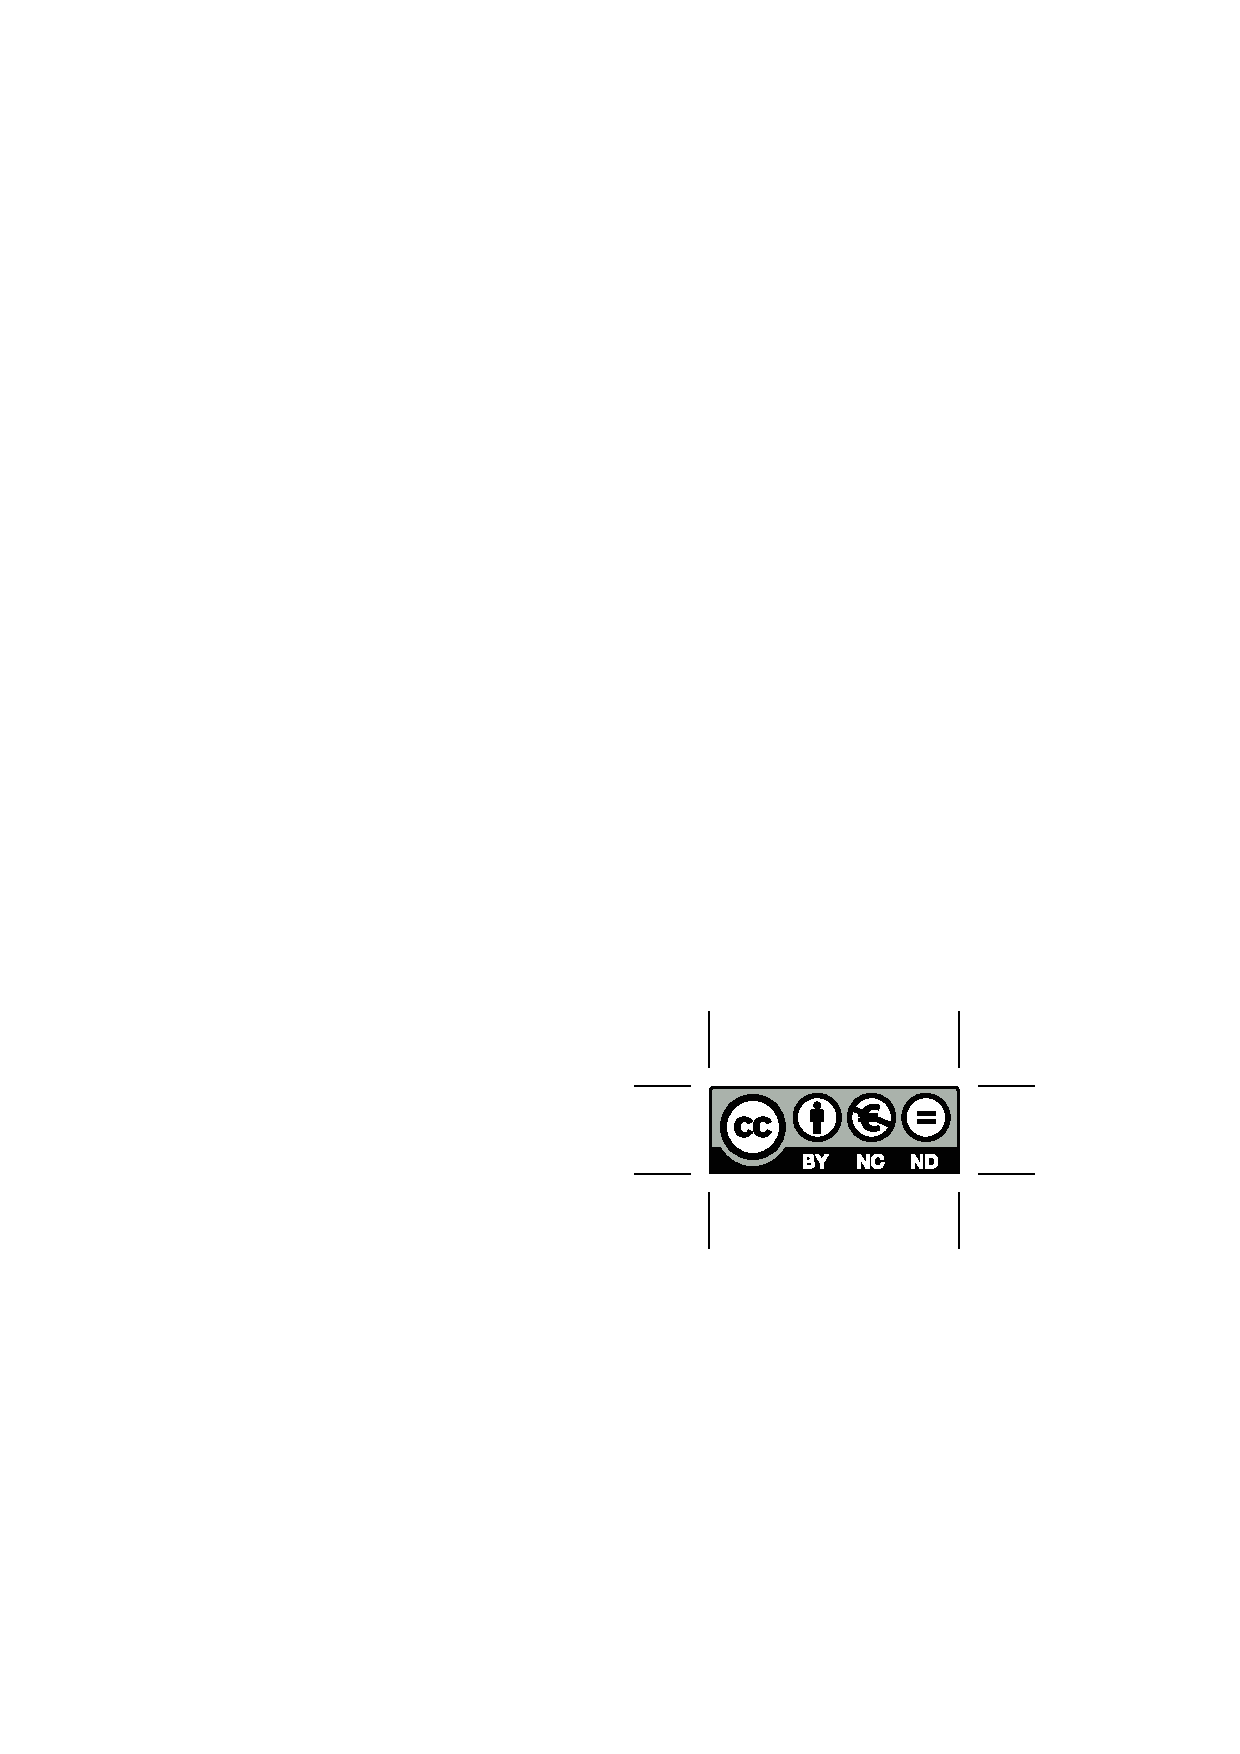
\includegraphics[height=1.3cm]{images_pdf/by_nc_nd_eu}
  \end{minipage}\hfill
\end{center}

Cette oeuvre est mise \`a disposition selon les termes de la \href{http://creativecommons.org/licenses/by-nc-nd/4.0/deed.fr}{Licence Creative Commons Attribution - Pas d'Utilisation Commerciale - Pas de Modification 4.0 International}. % consultez les conditions de la licence cc by-nc-nd, vous pouvez appliquer une licence moins restrictive, cc by-nc-sa par exemple


\clearpage
\pagestyle{fancyplain}

\parskip 0pt
\lhead[\fancyplain{}{\bfseries\thepage}]{\fancyplain{}{\bfseries Table\ of\ contents}}
\rhead[\fancyplain{}{\bfseries Table\ of\ contents}]{\fancyplain{}{\bfseries\thepage}}
\tableofcontents

\parskip 8pt

%%%%%%%%%%%%%%%%%%%%%%%%%%%%%%%%%%%%
% spacing for the main text
%%%%%%%%%%%%%%%%%%%%%%%%%%%%%%%%%%%%
\setlength{\parindent}{2.3em}
\setlength{\parskip}{1em}

%% Here is the summary in French
% no chapter or part header for the summary
\cleardoublepage
\begin{otherlanguage}{french}
\lhead[\fancyplain{}{\bfseries\thepage}]{\fancyplain{}{\bfseries R\'esum\'e en fran\c{c}ais}}
\rhead[\fancyplain{}{\bfseries R\'esum\'e en fran\c{c}ais}]{\fancyplain{}{\bfseries\thepage}}
%% This is the abstract of my dissertation, in French

\begin{center}
\underline{\textbf{\Large R\'ESUM\'E}}
\end{center}

Le projet ASTRID, réacteur nucléaire français de quatrième génération refroidi au sodium, est actuellement en cours de développement par
le Commissariat à l'énergie atomique et aux énergies alternatives (CEA). Dans ce projet, le développement de techniques de surveillance pour un réacteur nucléaire en
fonctionnement est identifié comme un problème majeur pour augmenter la sécurité du réacteur. L'utilisation de techniques de mesure par
ultrasons (par exemple thermométrie, visualisation d'objets internes) est considérée comme un puissant outil d'inspection des réacteurs rapides refroidis
au sodium, y compris ASTRID en raison de l'opacité du sodium liquide.

\`A l'intérieur d'un circuit de refroidissement au sodium, l'hétérogénéité du milieu se produit du fait de l'état d'écoulement complexe, notamment
lorsque le réacteur est en fonctionnement, et les effets de cette hétérogénéité sur la propagation des ondes acoustiques ne sont pas négligeables.
Ainsi, il est nécessaire d'effectuer des expériences de vérification pour les développements de technologies pour les composants, sachant que de telles
expériences utilisant du sodium liquide peuvent être des expériences à relativement grande échelle. C'est pourquoi les méthodes de simulation numérique
sont essentielles avant d'effectuer des expériences physiques en laboratoire, et en complément des résultats expérimentaux, qui sont nécessairement limités en nombre.
Bien que diverses méthodes numériques
aient été utilisées pour modéliser la propagation d'ondes acoustiques dans le sodium liquide, la communauté n'a toujours pas de méthode de modélisation de formes d'ondes complètes
qui soient bien validées dans le cas de modèles tridimensionnels de grande taille présentant des hétérogénéités.
De plus, à l'intérieur d'un coeur de réacteur, c'est-à-dire une région couplée acoustique-élastique
complexe, il est également difficile de simuler de manière précise de tels problèmes avec des techniques numériques qui soient basées sur du tracé de rais conventionnel.

L'objectif de l'étude menée dans le cadre de ma thèse est donc de contribuer à résoudre ces deux points en appliquant une méthode de calcul tridimensionnelle
par la technique numérique des éléments spectraux, qui est une
méthode d'éléments finis d'ordre élevé calculée dans le domaine temporel, qui peut modéliser nos objets d'étude (par exemple le milieu caloporteur sodium à l'intérieur du réacteur
nucléaire) de manière plus précise que les méthodes de simulation plus classiques.

Nous étudierons d'abord le potentiel de développement de la thermométrie ultrasonique dans un environnement sodium liquide fluctuant similaire à celui d'un
réacteur rapide refroidi au sodium, et étudierons si et comment la thermométrie ultrasonique peut être utilisée pour surveiller le flux de sodium à
la sortie du coeur du réacteur. Nous obtiendrons des variations de temps de vol claires dans le cas d'une faible différence de température de 1\% dans le cas
d'un gradient de température statique ainsi qu'en présence d'une fluctuation aléatoire du champ de température dans le flux turbulent. Nous
vérifierons que de petites variations de température dans le flux de sodium de par exemple environ 1\% de la température du sodium, c'est-à-dire environ 5 degrés
Celsius, peuvent avoir une signature acoustique mesurable de manière fiable. Pour ce calcul, le domaine cible sera modélisé comme un processus aléatoire
bidimensionnel et Gaussien appliqué pour générer une fluctuation de la température dans le sodium liquide.

Afin d'étudier l'hétérogénéité tridimensionnelle et des champs de température plus réalistes dans le milieu, dans un deuxième temps dans cette thèse nous effectuerons une seconde étude
numérique, cette fois-ci à trois dimensions. Pour représenter l'hétérogénéité du sodium liquide, nous appliquerons un champ de température quadridimensionnel (trois dimensions spatiale et une dimension temporelle)
calculé par modélisation numérique en dynamique des fluides avec une simulation LES (Large-Eddy Simulation) réalisée par CEA STMF au lieu d'une méthode conventionnelle
plus classique et moins chère (par exemple un processus aléatoire Gaussien). Nous montrerons qu'à partir de cette expérience numérique tridimensionnelle, nous
serons en mesure d'analyser les effets tridimensionnels de l'hétérogénéité réaliste dans le milieu de propagation sur les ondes acoustiques se propageant dans le sodium liquide,
dans une expérience de mélange de jets appelée PLAJEST.
Nous montrerons également que l'on peut déduire des mesures acoustiques des informations pertinentes pour des études de conception dans le domaine de la thermo-hydraulique :
fréquence des fluctuations de température, délimitation de la zone de plus fortes fluctuations de température, et température moyenne en fonction de l'altitude.


\end{otherlanguage}

%% Here is the summary in English
% no chapter or part header for the summary
\cleardoublepage
\lhead[\fancyplain{}{\bfseries\thepage}]{\fancyplain{}{\bfseries Summary in English}}
\rhead[\fancyplain{}{\bfseries Summary in English}]{\fancyplain{}{\bfseries\thepage}}
%% This is the abstract of my dissertation, in English

\begin{center}
\underline{\textbf{\Large SUMMARY}}
\end{center}

The ASTRID project, a French sodium-cooled nuclear reactor of 4th generation, is currently under development by the French Alternative Energies and Atomic Energy
Center (CEA). In this project, development of monitoring techniques for a nuclear reactor in operation is identified as an important issue to improve
the plant safety. The use of ultrasonic measurement techniques (e.g. thermometry, visualization of internal objects) is regarded as a powerful inspection tool
for sodium-cooled fast reactors, including ASTRID due to the opacity of liquid sodium.

Inside a sodium cooling circuit, heterogeneity of the medium occurs because of a complex flow state, especially when the reactor is in operation, and then the
effects of this heterogeneity on acoustic wave propagation are not negligible. Thus, it is necessary to carry out verification experiments for development of
component technologies, and such kind of experiments using liquid sodium may be relatively large-scale, i.e., difficult and expensive. This is a reason why numerical simulation methods
are essential before performing real laboratory experiments, or in addition to the number of experimental results, which is necessarily limited due to their
difficulty and cost. Though various numerical methods have been
applied to model wave propagation in liquid sodium, the community still does not have a verified and fully tested full-wave method for
numerical modeling of wave propagation in large-scale three-dimensional heterogeneous sodium reactors.
Moreover, inside of a reactor core i.e. in a complex acoustic-elastic coupled region, it is also difficult to simulate such problems with conventional ray-based
methods.

The objective of the study in the thesis is to contribute to solving these two points by resorting to a three-dimensional spectral-element method, which is a high-order
time-domain finite-element method that we will show to be suitable to model our targets (i.e. sodium coolant inside a nuclear reactor) more accurately
than more classical numerical simulation methods.

We will first study the development potential of ultrasonic thermometry in a liquid fluctuating sodium environment similar to that present in a Sodium-cooled
Fast Reactor, and thus investigate if and how ultrasonic thermometry could be used to monitor the sodium flow at the outlet of the reactor core. We will obtain
clear time-of-flight variations in the case of a small temperature difference of one percent in the case of a static temperature gradient as well as in the
presence of a random fluctuation of the temperature field in the turbulent flow. We will verify that small temperature variations in the sodium flow of e.g.
about \SI{1}{\percent} of the sodium temperature, i.e. about 5 degrees Celsius, can have a reliably-measurable acoustic signature. For this calculation, the
target domain will be modeled as a two-dimensional medium, and a Gaussian random process will be applied to generate fluctuations of temperature in the liquid sodium.

To investigate 3D heterogeneity and more realistic temperature fields in the medium, in a second part of the thesis we will carry out a numerical study
for 3D models of the reactor core. To represent the
heterogeneity of liquid sodium, a four-dimensional temperature field (three spatial and one temporal dimension) calculated by computational fluid dynamics based on
a Large-Eddy Simulation performed by CEA STMF will be applied instead of using a cheaper, more classical method such as e.g. a Gaussian random
process. We will show that based on that numerical experiment we will be able to analyze the 3D effects of realistic
heterogeneity in the propagation medium on the propagation of acoustic waves in liquid sodium, in a jet-mixing experiment called PLAJEST.
We will show that from acoustic measurements we can deduce information relevant to design studies in thermal-hydraulics: frequency of temperature variations, delimitation of the zone of greater fluctuation of temperature,
and average temperature with respect to altitude.


% done
\cleardoublepage
\lhead[\fancyplain{}{\bfseries\thepage}]{\fancyplain{}{\bfseries Chapter\ \thechapter \ -- \leftmark}}
\rhead[\fancyplain{}{\bfseries Chapter\ \thechapter \ -- \leftmark}]{\fancyplain{}{\bfseries\thepage}}
%
\chapter{Brief summary of the state of the art of ultrasound probing for liquid sodium}

In this chapter, let us introduce the general context of the thesis, and its main goals.
In \autoref{ssec:gen4} we will thus briefly recall some international research and development projects related to the new fourth-generation nuclear
reactors, which is the background of this thesis. Then in \autoref{ssec:ac_nuc} we will recall how ultrasound measurement techniques are
used in nuclear reactors. We will indicate methods that have been proposed in past research projects. In the following sections (\autoref{ssec:ac_char}), the acoustic
properties of the coolant medium (i.e. liquid sodium) of the SFRs are presented. The heterogeneous thermo-fluidal state of the medium in an operating
situation of the reactor is explained, referring to former studies, in \autoref{sec:stat_sod}. Finally the possible effects of heterogeneity of the medium
on acoustic wave propagation, which are discussed in the literature, and the objectives of this thesis will be explained (\autoref{ssec:fluc_mod} and \autoref{sec:goals}).

\section{Sodium-cooled fast reactors and the need for ultrasound measurements}

\subsection{The Generation-IV forum and ASTRID project} \label{ssec:gen4}

    Research \& development (R\&D) of next-generation nuclear power systems is being pursued under the "Framework agreement for international collaboration on
research and development of generation IV nuclear energy systems" by countries belonging to the Generation IV International Forum (GIF)
\citet{GIF2005Frameworkagreementfor}. Initially, in 1999, the United States advocated the concept of Generation-IV nuclear reactors and then proposed to other
countries to organize an international forum for international collaboration to develop fourth-generation nuclear power systems. In response to this, in July
2001, a charter that defines the principles of GIF was formalized by the Republic of Argentina, Brazil, Canada, France, Japan, the Republic of Korea, South
Africa, the United Kingdom and the United States. After subscriptions by the European Atomic Community (i.e. Euratom), People's Republic of China, Russia and
Switzerland, GIF is nowadays being operated by 12 countries and one international organization.

    Generation IV (Gen-IV) is defined as a new nuclear power system following the nuclear reactors at the beginning of nuclear reactor technology from the 1950's
to the first half of the 1960's (Gen-I), commercial light-water reactors built from the latter half of the 1960's to the first half of the 1990's (Gen-II) and their improved
versions from the latter half of the 1990's to the 2010's (Gen-III and Gen-III+). The objectives of GIF were clearly identified as:
    \begin{itemize}
     \item achieve sustainable development of nuclear energy by optimizing the use of natural uranium resources and by reaching the highest levels of nuclear safety,
     \item minimize the production of the most radioactive waste, in particular long-lived waste,
     \item ensure high resistance to nuclear proliferation,
     \item develop applications of nuclear energy for other uses than production of electricity.
    \end{itemize}
    After the analysis phase for designing plans, the GIF consortium selected six concepts of nuclear reactors that exhibited promising potentials to
achieve the above-mentioned objectives \parencite{GIF2014TechnologyRoadmapUpdate}.
    \begin{itemize}
     \item SFR: Sodium-cooled Fast Reactor
     \item GFR: Gas-cooled Fast Reactor
     \item LFR: Lead-cooled Fast Reactor
     \item SCWR: Supercritical Water-cooled Reactor
     \item VHTR: Very High Temperature Reactor
     \item MSR: Molten Salt Reactor.
    \end{itemize}
    Advantageous thermo-physical properties of the coolant, liquid sodium for SFR concept leading to normal atmospheric pressure, (i.e. high boiling point, heat of vaporization, heat capacity and thermal
conductivity) lead to a large safety margin for coolant boiling, and this contributes to important safety features of Sodium-Cooled Fast Reactors (SFRs), which
is one of the design purposes of Gen-IV nuclear reactors. Thus, SFR was adopted as one of the possibilities for Gen-IV, and its R\&D is carried out
internationally in France, Japan, Russia, USA, Republic of Korea and China. This limited number of countries implied in SFR explains the small number of international references
in the bibliography.

    Before GIF, the development of SFR has been undertaken in many countries through operations of several experimental, prototype and demonstration reactors,
for example Rapsodie, Phenix, SuperPhenix in France, PFR in the United Kingdom, BN-550, BN-600 and BN-800 in Russia and Monju and Joyo in Japan.
    In France, an R\&D project aimed at technological innovation concerning SFR has now been launched in collaboration with the French Alternative Energies and
Atomic Energy Commission (CEA), Areva (now called Framatome) and Electricity de France (EDF) in 2007. As a part of this global project, a first prototype industrial-sized SFR
development is ongoing. It is called the ASTRID project (Advanced Sodium Technological Reactor for Industrial Demonstration). This project pursuits four technical
targets \parencite{CEA20124thgenerationsodium}:

    \begin{figure}[htbp]
        \centerline{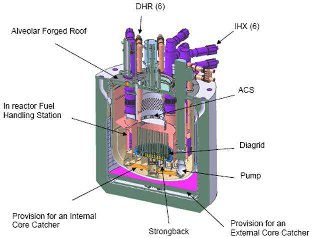
\includegraphics[width=10.0cm]{design_astrid.pdf}}
        \slantedcaption{
        Pre-conceptual design for the ASTRID reactor block (taken from \cite{Baque2015ASTRIDInService}).
        DHR: Decay Heat Removal system.
        IHX: Intermediate Heat Exchanger, which transfers heat from the primary coolant circuit to the secondary coolant circuit.
        ACS: Above-Core Structure, which supports the control rod drive mechanisms and core instrumentation, including the thermocouples etc.
        Internal/external core catcher: Collect and manage the corium (melted core and metallic structure) in case of a Core Disruptive Accident.
        Strongback: Structure in sodium coolant that supports the core.
        Diagrid: Structure that supports the subassemblies.}
        \label{fig:design_astrid}
    \end{figure}

    \begin{itemize}
       \item  Design of a high-performance core with improved safety: in particular, concerning prevention of severe accidents likely to cause complete core
meltdown,
       \item  Improved resistance to severe accidents and external aggressions: in particular, design of redundant and diversified decay heat removal systems,
as well as aspects related to the risk of re-criticality accident (i.e. uncontrolled nuclear fission chain reaction) and to molten core containment,
       \item  Search for an optimized and safe power conversion system intended to reduce or even completely remove the risk of interaction between sodium and
water,
       \item  Reactor design options to make inspection and maintenance easier and, more generally, to improve the availability, performance and general
economic characteristics of the facility
       (Figure \ref{fig:design_astrid} shows the pre-conceptual design of the planned ASTRID reactor).
    \end{itemize}
    Because of their high reactivity with sodium, the coolant circuit of SFR needs to be completely sealed from air and water, thus
further development of inspection and monitoring techniques are one of the keys for practical applications of SFR \parencite{GIF2014TechnologyRoadmapUpdate}.

\subsection{Ultrasound as a monitoring technique for ASTRID for in-service inspection and repair and for continuous surveillance} \label{ssec:ac_nuc}

    We give below a short summary of acoustic applications that are being developed in the framework of the ASTRID project (see e.g. \parencite{Giot2017Nuclearinstrumentationmeasurement}).
Similar developments have been or are being made in other frameworks; some of them will be reported in this dissertation.
    Schematically, two main reactor environmental conditions are to be considered:
    \begin{itemize}
    \item Operation periods, which are associated with high temperature (550\textdegree{}C approx.), high coolant flow, and high levels or radiation (neutron plus gamma),
    \item Shutdown periods, which are associated with lower temperature (200\textdegree{}C approx.), lower coolant flow, and lower levels of radiation.
    \end{itemize}
    In the field of applications, two domains are also classically considered:
    \begin{itemize}
    \item In-Service Inspection and Repair (ISI\&R), which is generally associated with the shutdown periods. Some typical applications are:
        \begin{itemize}
        \item non-destructive-evaluation, periodic inspection of welds,
        \item periodic inspection of structure integrity, locations and displacements of structures,
        \item imaging of objects and structures,
        \end{itemize}
    \item Continuous Surveillance (CS), which is generally associated with the operating periods.
    Some typical applications are:
        \begin{itemize}
        \item boiling detection in the primary circuit, and leakage detection in the secondary circuit,
        \item gas monitoring: sizing argon bubbles, and void fraction measurements,
        \item structure displacements,
        \item sub-assembly displacement monitoring,
        \item sub-assembly outlet temperature monitoring, ...
        \end{itemize}
    A third domain focuses on the refueling periods of the reactor, at shutdown conditions.
    Some typical applications are:
       \begin{itemize}
       \item monitoring of refueling operations versus mechanical conditions,
       \item monitoring of refueling safety versus subassembly characteristics and history, sub-assembly identification.
       \end{itemize}
    \end{itemize}

    The use of a sodium environment results in strong limitations in terms of available investigation techniques,
for the continuous surveillance / operation period conditions, as well as for the routine in-service inspection / shutdown period conditions (sodium draining is considered as an exceptional procedure, for the sake of repair for example).
    Sodium is a metallic element, with a high electrical conductivity and a magnetic behavior, and is rather opaque to electromagnetic waves.
    Magnetic and electrical fields can be induced at very short distances, for instance with Electromagnetic Acoustic Transducers (EMAT), to produce acoustic waves.
However, electromagnetic (including optical) and electrical techniques are unusable in sodium for long distance measurements, as mentioned above.

    Acoustic techniques have been regarded as convenient ones for the above purposes, in a passive "receiver" mode (noise detection of boiling and of leaks, generally at low frequencies), as well as in an active "transmitter-receiver" mode (telemetry-based measurements, generally at high frequencies).
Indeed, pure liquid sodium has rather good acoustic properties, with low attenuation and a moderate acoustic wave speed (about \SI{2400}{\meter\per\second}, with suitable wavelengths),
and acoustic techniques can thus be used in a broad frequency domain (currently up to 5 MHz for instance).
    Specific acoustic transducers have been and are still being developed to fulfill the shutdown and the operation physical conditions, as well as the acoustic specifications.

    It is known that temperature and flow heterogeneities and fluctuations will affect acoustic propagation (signal amplitude and signal-to-noise ratio, time of flight, path deflection, ...), with effects that increase with the propagation distance. These effects are far stronger in operation conditions than in shutdown conditions (which may be considered as isothermal and steady, in first stages of acoustic studies at least).

Our studies thus mostly focus on continuous surveillance conditions, and two representative applications, in the active mode, will be considered in \autoref{ssec:ac_prop} and in this dissertation:
    \begin{itemize}
    \item Ultrasonic temperature measurement at the outlet of fuel sub-assemblies (with possibly long propagation distances), which was the starting point for the studies of ultrasound propagation in heterogeneous sodium at CEA, and is studied in the general framework of SFR as a possible alternative to thermocouple-based measurements,
    \item Ultrasonic sub-assembly displacement monitoring (with shorter propagation distances), which has already been implemented in the Phenix reactor (using the SONAR device), and is studied in the framework of the ASTRID project as well.
    \end{itemize}
The description of this medium, from an acoustic point of view, is presented in the next section.

\section{Ultrasonic waves in liquid sodium}

\subsection{Properties of liquid sodium for ultrasound} \label{ssec:ac_char}

    To describe acoustic wave propagation in liquid sodium, it is necessary to know two main properties: density and wave speed. Both of them are temperature dependent.
    The characteristics of liquid sodium and its temperature-dependent properties were reported in \cite{Sobolev2011Databaseofthermophysical}. That study shows
that at normal atmospheric pressure, the density difference of liquid sodium with temperature change between the temperature range from the normal melting
point to the normal boiling point may be calculated with the linear relation:
    \begin{align}\label{eq:I_1}
        \rho\,[ \text{kg} \, \text{m}^{-3} ]=1014-0.235\cdot T\,[ \text{kelvin} ].
    \end{align}
    The sound speed of liquid sodium decreases monotonically with temperature, which is caused by decreasing of the inter-atomic interactions. In the range
of the normal melting - boiling point (\num{371}-\num{1155}\textdegree{}\si{\kelvin}), sound speed in pure liquid sodium may be described based on a linear relation:
    \begin{align}\label{eq:I_2}
        c_p\, [\text{m}\, \text{s}^{-1}] = 2723-0.531\cdot T\,[\text{kelvin}].
    \end{align}
    In this study, these two formulations are applied for acoustic properties of liquid sodium because the valid temperature range for these equations matches
the in-operation situation of the ASTRID.

    Because of these characteristics, an acoustic field may be influenced and modified by the heterogeneity of temperature in liquid sodium.
    A visualization of such modified acoustic rays can be found in the introduction part of published studies that are mentioned in the later part of this chapter (Figure \ref{fig:nicolas} in \autoref{ssec:fluc_mod} for instance).
    Variations of the acoustic impedance $Z$ ($Z=\rho c_p$) affect the transmission of ultrasonic waves (attenuation), and variations of the acoustic speed accelerate, decelerate or deviate the acoustic wave (refraction of the acoustic wave). This may lead to well-known undesirable effects when the amount of modification becomes large: degradation of the signal-to-noise ratio, focusing or defocusing of the acoustic beam, and creation of acoustic shadow zones.
What makes this matter very complex is the fact that the behavior of the heterogeneity changes spatially and temporally at the same time. Thus it is important to obtain information on the temperature state of a coolant flow when one designs acoustic devices for SFR.

%%% TODO add deflacted wave or path image

\subsection{Ultrasonic measurements in liquid sodium} \label{ssec:ac_prop}

    Several applications of acoustic measurement in liquid sodium have been studied in the literature.
    Thermometry (i.e. an acoustic telemetry technique for the measurement of temperature) is one of them. Monitoring the thermo-fluidal state of the coolant is
a very important perspective to reach a safe operation of nuclear reactors. Hence, for previous French reactors such as Phenix and Superphenix, measurement of
the sodium temperature at the core outlet was already performed based on thermocouples.

    Acoustic thermometry is not the only way to measure temperature of the upper core region i.e. the method using thermocouples, but acoustic thermometry may
be applied to SFR because of its advantages \parencite{Massacret2014Etudedunemethode}. One of the main advantages of this method is its ability to perform
high-frequency measurement; for acoustic measurements, there is no duration for heat transfer to the sensor through thermally-inert materials, which inevitably
occurs in the case of thermocouples. This ensures a very fast measurement, whose frequency may possibly be up to a few kiloHertz, which makes it possible to
monitor the fast temperature evolutions that may result from incidents or accidents. Another advantage of this method is that multiple locations on an acoustic
path may be measurable at the same time. This may reduce the number of measurement devices.

    Thermometry needs to use two reflections of an acoustic echo from reflecting objects that are present on the acoustic path. When distances between an
acoustic source and those objects are known, the average sound speed between the two objects may be calculated by
    \begin{align}\label{eq:I_3}
        c'_{ij}=\frac{2(d_i-d_j)}{t_i-t_j},
    \end{align}
    where $c'_{ij}$ is the average sound speed between the $i$-th and $j$-th reflective objects, $d_i$ is the distance from an acoustic source to the $i$-th object, and
$t_i$ is the so-called acoustic time of flight (TOF) i.e. the travel time from the emitter to the receiver. All reflection points and acoustic source are assumed to
be aligned. From equations \ref{eq:I_2} and \ref{eq:I_3}, the average temperature between two objects is estimated. Figure \ref{fig:tspatent} shows a drawing
of this concept of thermometry \parencite{McKnight1987Remotetemperaturemeasurement}.
Sub-figure A shows an application of an acoustic device (12) targeting multiple subassembly heads from above, and B shows a horizontal section view.
When the positions of the multiple subassembly heads are on a single acoustic ray, theoretically this configuration may measure the average temperature of the areas t1, t2 and t3.
C shows another example of application in which the acoustic transducer measures temperature in a single subassembly head.
If it is possible to change the angle of the transducer, a single device may measure temperature at multiple positions (D).
For 20 years, this technique was licensed as a U.S. patent no. US4655992A.
As one can see in Figure \ref{fig:tspatent}, one of the advantages of this technique is that local temperature values of multiple points
are measurable with a single acoustic device.
    \begin{figure}[htbp]
        \centerline{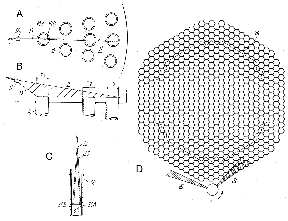
\includegraphics[width=13cm]{tspatent2.pdf}}
        \slantedcaption{Conceptual diagrams of thermometry, taken from \cite{McKnight1987Remotetemperaturemeasurement}.}
        \label{fig:tspatent}
    \end{figure}

    In 1992, ultrasonic thermometry was tested in the loop called HIPPO. HIPPO was a 1/2 scale representation of the core of a reactor of the European Fast Reactor (EFR) type
\parencite{Taylor1992Subassemblyoutlettemperature}. The objective of the experimentation was to observe the effects of a turbulent water flow on the
ultrasonic measurement of temperature at the outlet of sub-assemblies. The use of a core mock-up made it possible to determine the influence of subassembly
vibrations and potential false echoes occurring in the vicinity of assemblies. The fluid medium used in this experiment was water, and the subassembly outlets
were made of plastic. During the experiments, the flow rate in each assembly was 3.3 liter \si{\per\second}
(representing a flow speed of about \SI{1.5}{\meter\per\second}, half the real-life speed) and the water was at ambient
temperature in the whole loop. An \SI{5}{\mega\hertz} ultrasonic transducer was placed above the core and was aiming at an alignment of six
assemblies, as shown in Figure \ref{fig:hippo}. This transducer was similar to the transducers designed for actual EFRs.

    \begin{figure}[htbp]
        \centerline{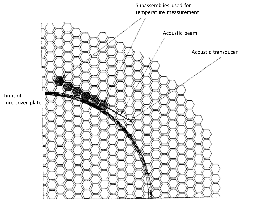
\includegraphics[width=12cm]{hippo.pdf}}
        \slantedcaption{Application of ultrasonic thermometry in the HIPPO loop, taken from \cite{Taylor1992Subassemblyoutlettemperature}.}
        \label{fig:hippo}
    \end{figure}
%
    It was verified that temperature measurement between the edges of the outlets of the sub-assemblies was possible with an uncertainty of only
$\pm$\num{0.6}\textdegree{}C, i.e. about \numrange{0.6}{2.0}\% of the average temperature (\numrange{10}{30} \textdegree{}C).
The result of this study \parencite{Taylor1992Subassemblyoutlettemperature} also indicates that
the ultrasonic measurement was not disturbed either by the flow of water nor by the potential assembly vibrations. It would have been interesting to determine
the influence of the size reduction of the geometry of the assemblies, which directly relates to the size of the thermal-hydraulic fluctuation patterns, on the
propagation of ultrasounds whose wavelength is full size (while the size of the sub-assemblies was half). Nevertheless, the accuracy of the temperature
measurements achieved by this technique, together with the absence of vibration effects, should encourage its implementation and further studies like ours.

The acoustic telemetry technique has also been used for the monitoring of the position of subassembly heads.
CEA for instance developed an acoustic measurement system called SONAR in order to study the generation mechanism of
four scrams by overpassing the reactivity threshold (an event called AURN) that occurred in the operation
of the French Phenix fast breeder reactor (FBR) \parencite{Berton1996Continuousmonitoringof}.
The objective of the SONAR system was to examine an hypothesis that AURN was caused by a small radial displacement of the subassembly.
SONAR measures the position of the subassembly head by tracking the change of time-of-flight
between the transducer surface and the subassembly head.

\begin{figure}[htbp]
    \centerline{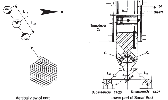
\includegraphics[width=10cm]{sonar_v2.pdf}}
    \slantedcaption{Image of the SONAR rod installation, taken from \cite{Berton1996Continuousmonitoringof}.}
    \label{fig:sonar}
\end{figure}

Figure \ref{fig:sonar} shows the description of the SONAR design.
The left image indicates the relation between the position of the SONAR rod and that of the target edges of the subassembly.
The right image is the cross-sectional image explaining the composition of the SONAR experiment.
There are multiple acoustic transducers in a rod.
C1 and C4 are used for measuring the time-of-flight to and from a subassembly edge.
The transducer C2 is used to measure the movement of the SONAR rod itself, caused by the flows.
As indicated in the left image, the acoustic ray does not pass through the central axis position of the sodium jets in this configuration,
but the effect of the medium heterogeneity occurs nonetheless for this position, as can be observed in the recorded signal in Figure~\ref{fig:sonar2}A.

\cite{Berton1996Continuousmonitoringof} show the measured signal fluctuation in the reactor at \num{550}\textdegree{}C.
The first curve in Figure \ref{fig:sonar2} is the estimated distance between the transducer and the subassembly edge for the C1 transducer.
The second curve is the measured distance between the C2 transducer and the wall of the sleeve, which indicates the movement of the SONAR rod.
The third curve is the estimated distance between C1 and the targeted subassembly edge, for which the effect of a change in the rod position is subtracted.
The noise in this curve gives an idea of the effect of thermo-hydraulic fluctuations in the SFR.
\cite{Fontaine2011Descriptionandpreliminary} studied deformation states of the subassembly and changes of fuel reactivity, and controlled the flowering (radial expansion) state
of a subassembly rod mechanically.
They measured the induced displacement of the subassembly head using the SONAR system in the Phenix reactor.
Figure \ref{fig:sonar2}B shows the radial displacement measured by the SONAR device versus their mechanical control states of subassembly flowering,
indicated as "Vertical piston position".
This is because, in the experiment device, the amount of flowering was controlled by the movement of a piston inserted in a test subassembly rod.
In this paper, the relation between the amount of flowering, the temperature of the sodium and reactivity is studied as well.
The sodium temperature was \num{350}\textdegree{}C.

\begin{figure}[htbp]
    \centerline{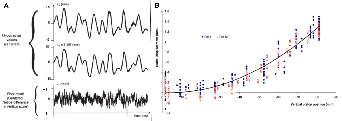
\includegraphics[width=16cm]{sonar2_v2.pdf}}
    \slantedcaption{Measured displacement of a subassembly head measured by SONAR, taken from \cite{Berton1996Continuousmonitoringof} (left) and \cite{Fontaine2011Descriptionandpreliminary} (right).}
    \label{fig:sonar2}
\end{figure}

As shown in \cite{Berton1996Continuousmonitoringof} and \cite{Fontaine2011Descriptionandpreliminary}, SONAR can thus measure small displacements of the tracked subassembly head.
The sensitivity of the measurement strongly depends on the noise created by the SONAR rod vibrations and by the thermal-hydraulic fluctuations.
Because the displacement is a short transient one, it is not possible to enhance the signal-to-noise ratio based on time-averaging techniques for example.
One must thus evaluate the error that thermal-hydraulic fluctuations can induce.
Also correcting vibratory perturbations, \cite{Berton1996Continuousmonitoringof} shows that measured distance fluctuation is
$\pm$ \SI{0.7}{\milli\meter} when the reactor is in operation (which is equivalent to a $\pm$ \num{10}\textdegree{}C temperature fluctuation).
Generally speaking, the sensitivity will depend on numerous factors:
position of the transducer, ultrasonic path (whether it passes through the hot sodium jets or not), sodium recirculation, size of the jets, and flow speed (which is itself
related to subassembly head design).
This is one of the reasons why numerical simulation can be a powerful tool to optimize devices involved in SFR studies.
One must also study the amplitude and shape of the echo, and study the elastic interaction between the subassembly head and the incident acoustic wave.
In the case of 3D circular head geometries with complex machined parts, an accurate 3D numerical simulation,
which could be performed based on the SPECFEM3D software package for instance, may be necessary.

\begin{figure}[htbp]
    \centerline{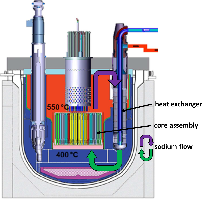
\includegraphics[width=10cm]{astrid_whole.pdf}}
    \slantedcaption{Sodium flow in the core of the current ASTRID conceptual design (taken from \cite{Barbier2017Mainoperationprocedures}).}
    \label{fig:astrid_whole}
\end{figure}

\section{State of the art of sodium flow modeling for SFR} \label{sec:stat_sod}

    In the sections above, application methods of ultrasonic monitoring for SFRs and ultrasonic properties have been briefly recalled.
Because of the dependency of sound speed on the medium temperature, as described,
it is crucial to understand the state of sodium circulation in order to estimate the usefulness and potential practical use of ultrasound measurements,
and in particular characterize the typical error levels that they can lead to for telemetry-based measurements in sodium flows.
In this section (\autoref{sec:stat_sod}), let us briefly review some of the latest studies on sodium flows in SFRs.
Pure thermo-fluid dynamical studies are cited because a thermo-fluidal
state is formed based on the history that the fluid has experienced. Our study concerns only the flow state of the upper-core region, i.e. the region located just above the
sodium outlet of the sub-assemblies. Three thermo-fluid studies will be recalled briefly in order to have knowledge on how sodium flows in the region of the core.

    \begin{figure}[htbp]
        \centerline{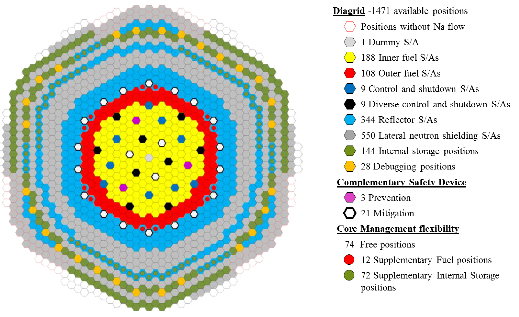
\includegraphics[width=15cm]{diagram_core.pdf}}
        \slantedcaption{Diagram for the planned ASTRID core assembly at the end of the conceptual design phase (taken from \cite{Venard2017TheASTRIDcore}).}
        \label{fig:diagram_core}
    \end{figure}
%
    In a SFR, the central part of the core is composed of hexagonal sub-assemblies that contain the nuclear fuel.
Figure \ref{fig:astrid_whole} shows the typical sodium flow in the primary coolant system,
and Figure \ref{fig:diagram_core} shows the diagram of the ASTRID core assembly at the end of the conceptual design phase.
The diameter of the core, including the reflectors, is about 7 meters, and the diameter of the vessel is about 16 meters.
The version of core design taken into account is
number four, and this version of the ASTRID core is called CFV version 4. The core assembly of version 4 is composed of 288 fuel sub-assemblies with a 17.17~cm pitch.
Each fuel subassembly includes 217 fuel pins. The diameter of the pins is 9.7~mm \parencite{Venard2017TheASTRIDcore}.
    Each pin is surrounded by helical wire spacers (Figure \ref{fig:subassembly}, B). In the core, the sodium flow orbits through the heat exchanger and core
assemblies driven by electromagnetic pumps. Inside the heat exchangers, thermal energy is passed to the secondary coolant system and then the temperature of sodium
decreases. This cooled sodium flow is heated again while the sodium flow passes through the sub-assemblies, which may have the highest temperature within
the entire cooling circuit, and which is exhausted from the subassembly heads.

    \begin{figure}[htbp]
        \centerline{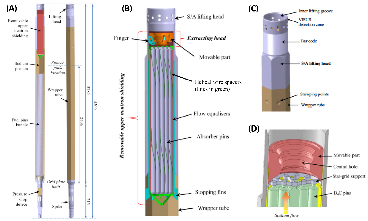
\includegraphics[width=17cm]{subassembly2.pdf}}
        \slantedcaption{Design of a subassembly. A: entire image and its cross-section. B: Neutron-shielding part. C: Subassembly head. D: Extracting head of
neutron shielding (taken from \cite{Beck2017Conceptualdesignof}).}
        \label{fig:subassembly}
    \end{figure}

    Because of the complexity of the geometry in which the sodium flow comes out, estimation for flow and heat transfer state is quite important for the
optimization of the SFR core, the subassembly design, and also for considering thermal fatigue. CEA has thus performed several numerical studies of core thermal
hydraulics of SFR by splitting them into three scales \citep{Gerschenfeld2017DevelopmentandValidation}:
    \begin{itemize}
        \item the global reactor scale, i.e. the reactor system scale,
        \item the local core scale, i.e. the individual subassembly scale,
        \item the scale of the other regions in which three-dimensional convection phenomena happen, excluding the subassembly part,
for instance the inter-wrapper gaps and the hot pool plenum.
    \end{itemize}
    This separation is currently unavoidable (in terms of computational cost) in order to be able to obtain the necessary resolution for the computation grids for each target and to maximize the volumes of the modeled domains.
    However, the interaction between the simulation of each of these scales needs to be considered because local scale phenomena may sometimes have a strong feedback effect
on the global behavior of the reactor \parencite{Gerschenfeld2017DevelopmentandValidation}.
In order to take into account all of phenomena with different scales and the interactions between them, CEA takes a calculation strategy that consists in
first computing the system-scale thermal-hydraulic states, based on a numerical code called CATHARE.
In a second step, the state of the local core scale is calculated
by taking into account the first system-scale simulation result as the initial condition.
For that step, the TrioMC code is used for the subassembly simulation, and another code called TrioCFD is used to compute the other regions in the reactor
in which three-dimensional convection occurs. Finally, once again the global-scale simulation is carried out with the data of local scale simulations
using a coupling code called MATHYS (Multi-scale ASTRID Thermal-HYdraulics Simulation).

    For example, \textcite{Saxena2014Thermalhydraulicnumerical} performed a numerical study for a subassembly of ASTRID (Figure \ref{fig:sim_subassembly})
to estimate the amount of pressure drop and hot spots (i.e. the place where temperature becomes high locally) happening around the supporting wires of fuel
pins. The pressure drop and hot spots may cause boiling of liquid sodium, and this may lead to local clad meltdown. In order to investigate the possibility of
occurrence of relatively small hot spots, \textcite{Saxena2014Thermalhydraulicnumerical} used a Large Eddy Simulation (LES) turbulent model in addition to a
Reynolds Averaged Navier-Stokes method (RANS) turbulent model.

    \begin{figure}[htbp]
        \centerline{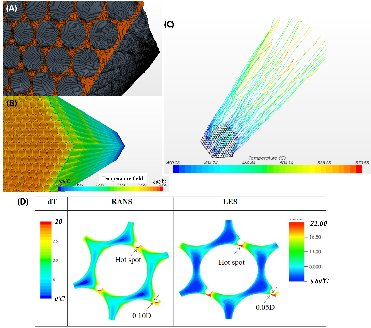
\includegraphics[width=12cm]{sim_subassembly_v2.pdf}}
        \slantedcaption{Thermal-hydraulic simulation for a subassembly made by \textcite{Saxena2014Thermalhydraulicnumerical}. A: Simulation mesh for a bundle of
fuel pins and spacing wires. B: Three-dimensional temperature field. C: Streamlines of flow with evolution of temperature (around the hexagonal can).
D: Calculated temperature difference in a cross section around a central fuel pin. The color map shows the difference of temperature based on the lowest
temperature of each cross section.}
        \label{fig:sim_subassembly}
    \end{figure}
%
    CEA is currently developing another code for the simulation of an individual subassembly model: the so-called TrioMC numerical simulation tool
(MC stands for the abbreviation of Core Model in French). This code allows one to calculate the temperature distribution of all cladding and sodium parts from a given mass flow rate.
    Figure \ref{fig:whole_core_by_trioMC}, taken from \cite{Conti2015Numericalanalysisof}, shows an example of calculation for sodium temperature of
sub-channels, i.e. spaces surrounding fuel pins, in a subassembly. The vertical axis indicates temperature values, and each color means the altitude in the
subassembly. This calculation estimates that a temperature gradient with a higher temperature at the center of the subassembly will be generated, and the radial
magnitude of the gradient will be maximum at the highest altitude, with $\Delta T$ about \num{60}\textdegree{}$C$ when $x= $\SI{0.08}{\meter}
(a more detailed figure can be found in \cite{Conti2015Numericalanalysisof}).

    \begin{figure}[htbp]
        \centerline{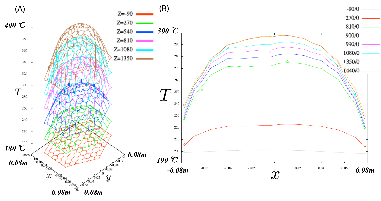
\includegraphics[width=14cm]{whole_core_by_trioMC_v4.pdf}}
        \slantedcaption{Temperature map calculated by the CEA numerical simulation code TrioMC.
A: Calculated (lines) and experimental (arrows) temperatures at each altitude of a subassembly.
B: Comparison on 2D intersections at several altitudes. The lines represent calculated values and the symbols represent experiment values. The $Z$ value is altitude in millimeters.
Taken from \cite{Conti2015Numericalanalysisof}.}
        \label{fig:whole_core_by_trioMC}
    \end{figure}
%
    After achieving the whole core temperature simulation, thermal-hydraulic calculations for the inter-wrapper and for the hot pool plenum zone are carried out by
coupling the results of the calculation of the sub-assemblies with a three-dimensional TrioCFD model (Figure \ref{fig:wholeCFD}). The thermo-fluid data for the
upper core region may then be numerically obtained, for the regions where ultrasound transducers will be installed (i.e., typically
the region shown with the purple rectangle in Figure \ref{fig:wholeCFD}).
This result illustrates the great technical and numerical challenge that needs to be addressed
to obtain quantitative information for ultrasound measurements in the upper core region,
as the above-core structure greatly modifies the sodium flow. As a result, the state of the flow and the distribution of the thermal gradient become heterogeneous.
From the temperature dependency, which has been recalled in \autoref{ssec:ac_prop}, these complex heterogeneities lead to uncertainty/difficulty of ultrasound measurements
in the upper-core region. This thesis will thus focus on how to try to compute and analyze such complexity and uncertainty.

    \begin{figure}[htbp]
        \centerline{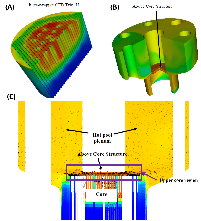
\includegraphics[width=17cm]{wholeCFD.pdf}}
        \slantedcaption{A,B: 3D TrioCFD model of inter-wrapper model and the hot pool plenum, including the upper-core region. C: Calculated temperature map
(color scale) and flow state (arrows). Taken from \cite{Conti2015Numericalanalysisof}.}
        \label{fig:wholeCFD}
    \end{figure}
%
    A more detailed numerical study on the flow state at a subassembly head was carried out by \textcite{Beck2017Conceptualdesignof}. The aim of that study was
design optimization of pins configuration and geometry of the extraction head (Figure \ref{fig:subassembly}). In Figure \ref{fig:cfd_head}, pre-optimization and
optimized geometry and simulated flow and temperature fields are shown. From the results for the pre-optimization geometry, the maximum difference of temperature at the
position of the monitoring system (A.2-2) is about \num{20}\textdegree{}$C$.
From the results for the optimized geometry, the size of the temperature gradient (B.2-2) at the same position is about \num{7}\textdegree{}$C$
and the velocity magnitude field (B.1-2) is more homogeneous than the pre-optimization result (A.2-1).
    We consider that, in reality, the state of the sodium flow becomes more complex than these calculation results
because of the effect of mixing with colder sodium around the outlet of a subassembly, and also because of convection.
Let us also mention that a Reynolds Averaged Navier-Stokes (RANS) model is used as the turbulent model, which means that the resulting size of the
heterogeneities is averaged for the point of view of ultrasounds, i.e. the size of the wavelength being much smaller than the resulting size of heterogeneities in the CFD results
for a sodium flow in the SFRs that are currently available.

    \begin{figure}[htbp]
        \centerline{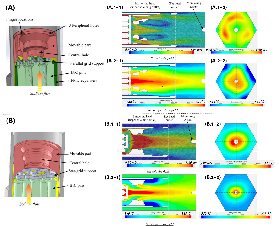
\includegraphics[width=17.9cm]{cfd_head_v3.pdf}}
        \slantedcaption{Geometry A: before optimization of an inner head of a subassembly; cross-sectional flow field (A.1-1) and temperature field (A.2-1) in the
long axial direction, and velocity magnitude field (A.1-2) and temperature field (A.2-2) in a perpendicular cross-section at the position of the monitoring system,
i.e. at the place where the thermocouples and flow-meter are located. B: after optimization: cross-sectional flow field (B.1-1) and temperature field (B.2-1) in the long axial direction,
and velocity magnitude field (B.1-2) and temperature field (B.2-2) in a perpendicular cross-section, taken from \textcite{Beck2017Conceptualdesignof}.
The inner diameter of the head is \SI{15}{\centi\meter} and the length of the cylindrical part (not hexagonal) of the head (i.e. from the left boundary of the A.1-1 image to the "S/A head outlet" part) is \SI{27}{\centi\meter}.}
        \label{fig:cfd_head}
    \end{figure}

    The latest numerical analysis, which was carried out by CEA for the upper core region and the hot pool plenum at nominal reactor power, shows that the possible radial flow rate is
about \SI{4.5}{\meter\per\second}, and the maximum variation rate of radial temperature is about \num{23.4}\textdegree{}C par \SI{10}{\centi\meter}
\parencite{Haubensack2016Calculsthermohydrauliquesdu}. It also shows that the modification of the acoustic field depends on the three-dimensional angle
and curvature of the temperature gradient versus a direction of an acoustic propagation ray.
    For this reason it is necessary to take into account the medium heterogeneities to ensure the accuracy of acoustic measurement methods
\parencite{Massacret2014Etudedunemethode}.
%
    The main objective of this thesis is thus going to be to study how an acoustic wave propagates in a model of a sodium flow that has realistic heterogeneity.

\section{Thermal-hydraulics studies with fluctuation of sodium jets, and acoustic point of view}

    As mentioned above, several thermal-hydraulic studies on the state of the sodium coolant fluid in the primary circuit of SFR have been carried out in the
literature. These studies, except \textcite{Saxena2014Thermalhydraulicnumerical}, use the Reynolds-Averaged Navier-Stokes (RANS) model for their
turbulence model for the upper core domain, which is the place on which we want to focus in this thesis.
    Turbulence models generally used for computational fluid dynamics (CFD) may be broadly divided into three types: RANS, Large-Eddy Simulation (LES),
and Direct Numerical Simulation (DNS). The appropriate model to use in a given situation is selected based on the purpose of the simulation (for instance the level of accuracy needed etc.)
and the amount of computer resources required:
%
\vspace{-4mm}
    \begin{itemize}
    \item RANS divides the flow variables (i.e. velocity, pressure and temperature) into a time-averaged part and a fluctuating part (a process called
Reynolds decomposition), and then a time-averaged thermo-fluid field is calculated,
    \item LES defines a cut-off threshold on the spatial size. Eddies larger than this threshold are calculated directly, and the smaller eddies are
modeled and calculated as more isotropic ones than those directly calculated,
    \item DNS solves the set of equations without any approximation, thus this model has the highest resolution and accuracy among these three models. However this method
requires enormous amounts of computer resources and this is why the application of DNS for the analysis of a whole nuclear core or a large part of a nuclear
core is currently still not feasible (but will become feasible one day).
    \end{itemize}

\vspace{-4mm}
    Figure \ref{fig:turbulent_models} shows the schematic representation of turbulent models and numerical results of each model
(\cite{Poitou2009Modelisationdurayonnement}, \cite{Saxena2014Thermalhydraulicnumerical}).
From this figure it is clear that a RANS-based simulation would not give a description of the temporal fluctuations of the jets.
    The acoustic wavelength of \SI{1}{\mega\hertz}, which is one of the possible acoustic frequencies considered to be used in the ASTRID core, is small:
approximately \SI{1}{\milli\meter} in the operating situation. This is the reason why a thermal-hydraulic field that would be averaged too much
may sometimes not be suitable to perform realistic acoustic simulations, because the spatial and temporal resolutions of averaged thermal-hydraulic results
are coarser than the resolution of the acoustic simulations.

    As we recalled in the previous sections, in the upper core region, hot sodium jets, which have a temperature within the range \num{450}\textdegree{}C (control rod) to \num{550}\textdegree{}C (hotter subassembly), and ambient
sodium, which may be \num{50}\textdegree{}C colder than the hottest jets, are mixed. This can cause complex and poorly known thermal-hydraulic phenomena.
For this reason, several studies exist on the thermo-fluidal fluctuation of sodium jets. The main purpose of these studies is the observation of a mixing phenomenon in the jets
of liquid sodium, and estimation of thermal fatigue of the metal material that is present in a SFR core. In those studies, the thermal fluctuation cycle is investigated in
details, thus we may use these results for our acoustic studies, as there are similarities with the objectives of our study.

    \begin{figure}[htbp]
        \centerline{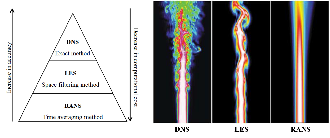
\includegraphics[width=12cm]{turbulent_models.pdf}}
        \slantedcaption{Left: Schematic representation of the three classical types of turbulent models used in numerical simulations.
Right: modeling of a flame. Taken from \cite{Poitou2009Modelisationdurayonnement} and \cite{Saxena2014Thermalhydraulicnumerical}.}
        \label{fig:turbulent_models}
    \end{figure}

\vspace*{-7mm}
    \begin{figure}[htbp]
        \centerline{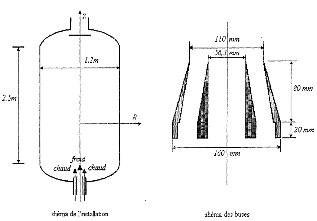
\includegraphics[width=12cm]{najeco_v2.pdf}}
        \slantedcaption{Test section of the NAJECO loop (taken from \cite{Tenchine1994Jetscoaxiaux:}).}
        \label{fig:najeco}
    \end{figure}

\vspace*{-3mm}
\subsection{The NAJECO experiment}

    In order to determine the characteristic length $L_{\theta}$ of these thermal heterogeneities in different fluids, \cite{Tenchine1994Jetscoaxiaux:} and
\cite{Tenchine1994Jetscoaxiaux:a} performed several experiments in the NAJECO and AIRJECO test loops. The objective of these experiments was to determine the
similarities between the thermal fluctuations of a flow of sodium and a flow of air and to determine if air is appropriate for the simulation of sodium with
temperature heterogeneity. To this end, the two test sections had identical geometries and generated coaxial fluids at different temperatures.

    For the NAJECO experiment, the two concentric sodium jets have different temperatures and flow rates: \SI{150}{\cubic\meter\per\hour} at
\num{280}\textdegree{}C and \SI{30}{\cubic\meter\per\hour} at \num{200}\textdegree{}C. The trial section of this loop is represented in Figure \ref{fig:najeco}.
    This test section generates two coaxial jets at different temperatures, and thus generates thermal heterogeneities that can be encountered at the
subassembly outlet, mainly where the coaxial jets from sub-assemblies and inter-sub-assemblies mix. The study of this experiment makes it possible to better
understand which types of heterogeneities may develop above the reactor core.

    In this experiment, a thermocouple was placed with the aid of a pole at different points of the flow, which made it possible to record temperature
fluctuations, to measure the spectrum of the thermal fluctuations, and to deduce the characteristic lengths of the flow.
    Table \ref{table:najeco} shows the results of this experiment at a distance of \SI{0.05}{\meter} from the sodium outlet.
    $U$ is the speed of the flow at the measurement point and $R$ is the distance from the measurement point to the vertical axis (Figure \ref{fig:najeco}).
    The characteristic length of the temperature fluctuation $L_{\theta}$ is calculated from the measured values based on
    \begin{align}\label{eq:I_4}
        L_{\theta} = \frac{U}{2\pi f_{\theta}},
    \end{align}
    where $f_{\theta}$ is the peak frequency of the measured temperature temporal fluctuation.

    \begin{table}
        \centering
        \slantedcaption{Characteristic length of the thermal heterogeneities at different points of the flow, 50~cm above the nozzles
(taken from \cite{Tenchine1994Jetscoaxiaux:}).}
\vspace{5truemm}
        \begin{tabular}{lll}
        Radius $R$ [\si{\meter}] & Speed $U$ [\si{\meter\per\second}] & Length $L_{\theta}$ [\si{\meter}] \\ \hline
        \num{0}              & \num{1.05}                 & \num{0.037}                    \\
        \num{0.016}          & \num{1}                    & \num{0.039}                    \\
        \num{0.04}           & \num{0.8}                  & \num{0.032}                    \\
        \num{0.10}           & \num{0.3}                  & \num{0.024}                    \\
        \end{tabular}
        \label{table:najeco}
    \end{table}

    Thus, for a sodium flow of this type, the characteristic length of the thermal heterogeneities \SI{50}{\centi\meter} above the tubes discharging the sodium
ranges between \SI{2}{\centi\meter} and \SI{4}{\centi\meter}. It is also important to note that heterogeneity size decreases with increasing distance between
the measurement point and the center of the flow. To understand why these variations occur, radial and axial measurement of the temperature fluctuations were
performed in the NAJECO experiments; the results are presented in Figure \ref{fig:najeco_res}.
    This profile indicates that most of the thermal fluctuations do not occur in the axis of the exit flow but rather on a ring centered on the flow, where the two
coaxial jets mix. On both sides of this ring the temperature heterogeneities are thus smaller. It should be noted that these profiles are also given far from
the jet outlets (\SI{50}{\centi\meter}).

    These results show that in spite of the high thermal conductivity of sodium, which tends to homogenize the medium temperature,
thermal heterogeneities can be observed as a result of the flow velocity field. These experimental results would not be simply compared to the expected SFR
sodium flow, as the direction of the flows are not identical.
Nevertheless it is likely that, in a horizontal plane very close to the subassembly outlet, circular homogeneous temperature zones can be observed,
their radius being of the order of that of the assembly. These zones would be separated by zones in which the temperature fluctuations
are large and the characteristic size of the temperature heterogeneities is about a few centimeters.

    It should also be noticed that these experiments were run without any obstacle and high above the jet outlets, the flows implemented here being different
from those implemented in the case of a actual reactor in which sodium flows are disturbed by the upper-core structures situated about 40~cm above the assembly
outlet. The findings of this study may therefore be modified by the presence of the upper-core structures. More precise knowledge of the flow above the core
will be necessary to conclude on the presence of a small disturbed zone above the assemblies.

    \begin{figure}[htbp]
        \centerline{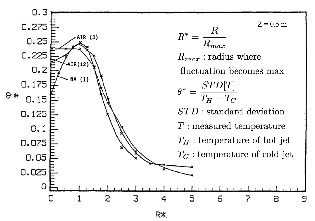
\includegraphics[width=13cm]{najeco_res_v4.pdf}}
        \slantedcaption{Radial profile of the intensity of the fluctuations in sodium, indicated as NA(1), and in air, indicated as AIR(3) and AIR(12), at altitude $Z$ = \SI{0.5}{\meter}
(taken from \cite{Tenchine1994Jetscoaxiaux:}).}
        \label{fig:najeco_res}
    \end{figure}

    \begin{figure}[htbp]
        \centerline{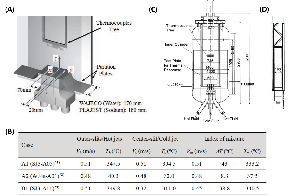
\includegraphics[width=16.2cm]{plajest_jaea_v2.pdf}}
        \slantedcaption{Geometry of the PLAJEST experiment (A,C,D) and three different initial conditions of the flow state (B), taken from \cite{Kobayashi2015Proposalofbenchmark}.
Water (A2) and sodium (A1, B1) are used for each medium.}
        \label{fig:plajest_jaea}
    \end{figure}

\subsection{The PLAJEST experiment, and numerical modeling based on large-eddy simulation}
\label{ssec:PLAJEST}

    Another program, called PLAJEST, is a collaboration between the Japanese Atomic Energy Agency (JAEA), the U.S. Department of Energy (DOE), and CEA in France.
The main purpose of PLAJEST is to observe heat conduction at a liquid-solid boundary in a sodium cooling circuit, because the thermal fluctuations lead to
high-frequency thermal fatigue and thus possibly to cracks in adjoining structures of SFRs. The configuration of this experiment is shown in Figure
\ref{fig:plajest_jaea}. After the experiment made by JAEA \citep{Kimura2005Studyonconvective,Kimura2008Studyonthermal}, thermo-fluid analysis was
done by CEA in its Service de thermo-hydraulique et de m\'ecanique des fluides (STMF) (\cite{Angeli2015LargeEddySimulation}, Figure \ref{fig:plajest_cea}). In that analysis, the results A and B indicate a good fit on time-averaged
normalized temperature (A) and its fluctuation (B) between experimental and numerical values. Moreover the power spectral density curves of temperature at the
middle point of the domain under study also exhibit a good fit (D).

    While these PLAJEST studies are not based on ultrasound propagation, and we did not carry out an acoustic experiment with the PLAJEST configuration
in this thesis, we will use the thermo-fluid computation results of case A1 as a CFD simulation results that is well validated by the experiment for our
full-wave propagation numerical simulations (in Chapter \ref{chap:3}) in realistic conditions.
CEA/STMF used a Large-Eddy Simulation turbulence model for this simulation, thus we may utilize these temperature fields with higher spatio-temporal resolution.

\subsection{Thermal fluctuation models used in previous acoustic studies in the literature} \label{ssec:fluc_mod}

    In previous studies published in the literature on acoustic wave propagation in heterogeneous liquid sodium,
a stochastic modeling was always applied for modeling of medium fluctuations
and heterogeneities of sodium flow in SFRs, because pertinent thermal-hydraulic input data were not available, and/or because realistic numerical modeling was too complex
or too expensive to perform. This stochastic method is still the fastest and cheapest way to prepare a
fluctuating acoustic propagation medium. Several such studies are briefly recalled in this section.

    David Fiorina, in his PhD thesis \parencite{Fiorina1998Applicationofthe}, generated fluctuating fields of sound velocity based on isotropic and homogeneous
Gaussian random processes in 2D.
This technique allows for a high-resolution representation of random variations in the propagation medium (\parencite{VladimirE.Ostashev2015AcousticsMovingInhomogeneous}).
He studied the effects of this heterogeneity in the propagating medium on an acoustic wave using a Gaussian beam summation
method. A point and line source were used in his calculation, and he analyzed the effect on the acoustic rays, time-of-flights, and variance of sound intensity
(Figure \ref{fig:fiorina}). In that simulation, the medium used was water. The average temperature was \num{30}\textdegree{}C, and variance of the temperature
was \num{25}\textdegree{}C with $L_{\theta}=0.03\, \text{m}$. He concluded that when the propagation distance is shorter than about \num{34} times the value of
$L_{\theta}$ (the characteristic length of heterogeneities), the simulated curve and the theoretical solution are in very good agreement. However, when the propagation distance
becomes longer than that length, the difference between the analytical solution and the result of the calculation becomes larger.
Let us mention that in this thesis, a Gaussian random process following this approach will be used in Chapter~3.

    Then, \textcite{Iooss2000Statisticalmomentsof} extended this method to a geometrically-anisotropic homogeneous Gaussian random process in 2D. This
extension was motivated by the demand coming from the fact that the fluctuation pattern is not isotropic when the flow velocity is not small. The Gaussian beam
summation method was again applied in that study, and the case of a plane wave and then a spherical wave were examined as types of acoustic emission.
Figure \ref{fig:iooss} shows the isotropic temperature and flow velocity fields (A) and anisotropic sound celerity field (B).
In \textcite{Iooss2002Numericalsimulationof} the authors concluded that:
    \begin{itemize}
        \item  In 3D modeling, the effects of the mean and turbulent fields are theoretically stronger on the travel times than in 2D modeling,
        \item  A fluctuating pattern generated based on a stochastic model is far from realistic fluctuating patterns,
        \item  Deterministic fluid mechanics can provide realistic temperature and velocity fields.
    \end{itemize}

    \begin{figure}[htbp]
        \centerline{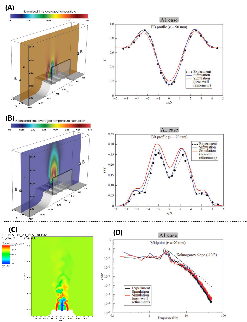
\includegraphics[width=17cm]{plajest_cea_v2.pdf}}
        \slantedcaption{Computational Fluid Dynamics results for the A1 case of the PLAJEST experiment configuration, obtained by \cite{Angeli2015LargeEddySimulation}.
A: Time-averaged normalized temperature field and
comparison with experimental data. B: Time-averaged normalized temperature fluctuation and comparison with experimental data.
C: Example of a non-time-averaged temperature field at a given time. D: Power spectral density curve at the middle point of the studied domain.}
        \label{fig:plajest_cea}
    \end{figure}

    \begin{figure}[htbp]
        \centerline{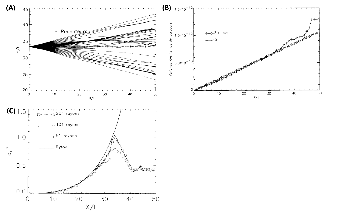
\includegraphics[width=17cm]{fiorina.pdf}}
        \slantedcaption{Results of a Gaussian summation simulation obtained by \textcite{Fiorina1998Applicationofthe}. A: Calculated acoustic rays emitted from
a point source. The value of each axis is divided by the characteristic length of fluctuations $L=L_{\theta}$. B: Variance of time-of-flights versus
propagation length. C: Normalized variance of fluctuations of sound intensity ($\sigma_T(\bm{x})^2=\sum_i(I_i-I_{average})/I_{average})^2, I_i=p_i*|\bm{v_i}|,
i: \text{index for } $x$ \text{ positions}, p: \text{pressure}, \bm{v}: \text{velocity vector}$) versus propagation length, compared with Rytov approximation \cite{Beydoun1988FirstBornRytov}. Taken from
\textcite{Fiorina1998Applicationofthe}.}
        \label{fig:fiorina}
    \end{figure}

    \begin{figure}[htbp]
        \centerline{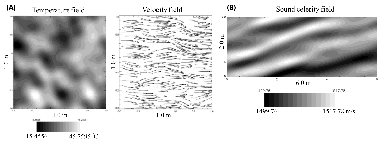
\includegraphics[width=17cm]{iooss_v4.pdf}}
        \slantedcaption{A: An example of isotropic temperature and flow velocity fields of water. B: Anisotropic sound celerity field in liquid sodium.
The velocity of the ambient flow is \SI{16}{\meter\per\second} tilted at \num{11.5}\textdegree{}. Taken from \textcite{Iooss2000Statisticalmomentsof}.}
        \label{fig:iooss}
    \end{figure}

    \cite{Lue2011Modelisationdela} and \textcite{Lue2012Stochasticsimulationof} applied a Gaussian random process to 3D simulation, and also proposed to apply
the Gaussian random process not to the generation of a physical quantity field (i.e. temperature and flow velocity field) but rather to the propagation field
(i.e. times of flight and acoustic amplitudes) itself. In these works, the propagation field is first calculated as wave propagation in a homogeneous medium,
and then the heterogeneous effects are calculated in transversal planes (Figure \ref{fig:bo} A) as a function of propagation distances, and then added to
the homogeneous fields.
Figure \ref{fig:bo}B shows an example of time-of-flight fluctuations in the transversal plane at a distance from the source of $30 l_\epsilon$,
where $l_\epsilon$ is the characteristic length of the medium fluctuations.
Sub-figure~C is an example of a fluctuating acoustic field calculated based on the stochastic model that we use.
A circular transducer with diameter \SI{30}{\milli\meter} was used.
The source signal is a Gaussian-modulated sinusoidal pulse with a dominant frequency of \SI{2}{\mega\hertz}.
D: Profiles of amplitude at $x$ = \SI{1.4}{\meter} extracted from the results presented in~C.
The red curve shows the result obtained in the case of homogeneous medium conditions.

\textcite{Lue2012Stochasticsimulationof} called this method a stochastic method.
The stochastic method provides faster generation of the fluctuating propagation field than a deterministic method.
The size of the calculated volume in that work is \SI{0.1}{\meter} < x < \SI{1.4}{\meter} and \SI{-0.05}{\meter} < y < \SI{0.05}{\meter}, with 2000 calculation points.
For the deterministic model the calculation time was about \SI{1.5}{\hour}, while for the stochastic model it was only \SI{10}{\second}, i.e., more than 500 times cheaper.
The results taken from that paper and presented in Figure~\ref{fig:bo}~D show a mean deviation of about \SI{10}{\milli\meter}
and a standard deviation of about \SI{7.6}{\milli\meter} at $x$ = \SI{1.4}{\meter}.
Let us mention that the stochastic method in \textcite{Lue2012Stochasticsimulationof} was validated using a ray-tracing technique.

    \begin{figure}[htbp]
        \centerline{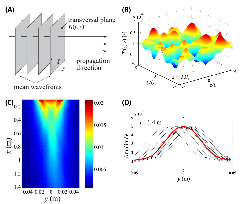
\includegraphics[width=17cm]{bo_v2.pdf}}
        \slantedcaption{
            A: Definition of the transversal plane on which the fluctuating part of a propagation field is calculated.
            B: Time of flight fluctuation on a transversal plane.
            C: One of fluctuating acoustic field calculated based on the stochastic model.
            D: Profiles of Amplitude at x = \SI{1.4}{\meter} extracted from C.
            Taken from \textcite{Lue2012Stochasticsimulationof}.}
        \label{fig:bo}
    \end{figure}
%
    \textcite{Massacret2014Etudedunemethode} simulated wave propagation just above the heads of the sub-assemblies under the assumption that in this region the
fluctuation of the medium is weak enough and can thus be ignored.
    The only heterogeneity taken int account is a static heterogeneous temperature that creates a temperature gradient along the wave path.
    His results show that under such an assumption, acoustic rays may be affected significantly and deviated (Figure \ref{fig:nicolas}). A ray-tracing code
called AcRaLiS was developed for this simulation. To describe the temperature field, the author performed an interpolation of the physical values of the field
onto the spatial points that are used for the ray-tracing calculation using a Delaunay triangulation.
    \textcite{Massacret2014Etudedunemethode} also applied the temperature and flow velocity map calculated for the PLAJEST experiment based on a RANS turbulent model (see the above section)
and obtained estimates of the change of times of flight for the wave front.
    \begin{figure}[htbp]
        \centerline{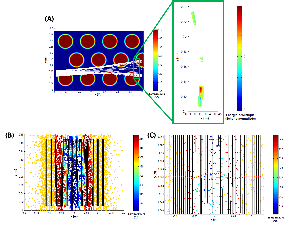
\includegraphics[width=17.9cm]{nicolas_v2.pdf}}
        \slantedcaption{A: Acoustic rays obtained based on a ray-tracing simulation code called AcRaLis above the subassembly heads without fluctuations (left)
and acoustic energy 63~cm away from the acoustic source (right). B: Deviated acoustic rays calculated with a temperature field obtained from the PLAJEST
simulation data. C: Plotted wave front. Taken from \textcite{Massacret2014Etudedunemethode}.}
        \label{fig:nicolas}
    \end{figure}

    To finish the overview of previous studies, let us mention some studies currently being performed in Belgium.
    SCK-CEN, the Belgian Nuclear Research Center is currently developing MYRRHA, a Generation-IV liquid-metal-cooled research nuclear reactor
\parencite{AitAbderrahim2012MYRRHAAmulti}. Lead-bismuth eutectic, which is also optically opaque, is used as the coolant medium in this reactor.
    In this project, one of the possible applications of the acoustic measurement technique is the detection and localization of potentially lost fuel assemblies.
For this purpose, the acoustic propagation distance may be about \SI{2.5}{\meter} and thus the effects of the heterogeneous temperature and velocity fields
on acoustic wave propagation need to be examined.
    To do this, \textcite{VandeWyer2014Experimentalandnumerical} developed an experimental facility called TAUPE. Water is used as the propagation
medium in that experiment (Figure \ref{fig:taupe} A,B). The corresponding medium, in terms of flow velocity and temperature gradient, were simulated in TAUPE,
and acoustic wave propagation was observed by means of acoustic signal and shadow-graph visualization.
    The authors of this experiment also developed a ray-tracing code and validated it based on their experimental results.
    They concluded that their ray-tracing code estimates the effects of temperature gradients on wave propagation accurately (Figure \ref{fig:taupe} D),
while the effects of the flow velocity field are overestimated. As \cite{Massacret2012Simplifiedmodelingof}, they also concluded that the effect of the flow velocity field
is negligible but that the effect of the temperature gradient is not negligible when the propagation distance is greater than about \SI{2.5}{\meter},
which is the required length for object detection and visualization.

    \begin{figure}[htbp]
        \centerline{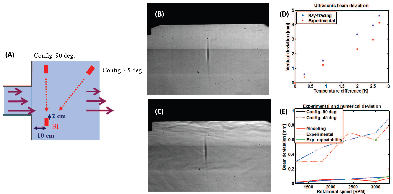
\includegraphics[width=17cm]{taupe_v2.pdf}}
        \slantedcaption{A: Configurations of the TAUPE experiment. S1 is the emitter. Two angles of acoustic propagation direction are examined.
B: Visualized wavefront in water without a temperature gradient nor velocity field. C: Visualized wavefront in water with a temperature gradient and velocity field.
D: Comparison between experimental results
and calculations made based upon a ray-tracing code, depending on the temperature gradient. E: Comparison between experimental results
and calculations made based upon that ray-tracing code, depending on the rotation of the flow generator.
Taken from \textcite{Wyer2015Theeffectof}. The authors find that the amount of (vertical) beam deviation increases when the magnitude of the temperature gradient becomes larger.
The same trend is also found when the rotational speed of the flow generator becomes faster, i.e. when the flow speed becomes faster.}
        \label{fig:taupe}
    \end{figure}

\section{Summary of the main goals of this thesis} \label{sec:goals}

    The main goals of this thesis are thus:
    \begin{itemize}
        \item The development and application of a full-wave propagation numerical method for the numerical analysis of acoustic wave propagation in the sodium coolant of a SFR,
for the first time in the literature to our knowledge. We selected the spectral-element method (SEM), which is a type of high-order time-domain finite element method.
As described above, to our knowledge only ray-based methods have been applied so far in the literature for acoustic wave propagation in such a medium,

        \item Improving the sodium flow description to take into account spatial fluctuations of the medium at the ultrasonic scale,

        \item Using the latest development of CFD calculations for sodium flows made by Service de thermo-hydraulique et de m\'ecanique des fluides (STMF) at CEA, we will study the effect of not only taking into account a 3D environment but also
temporal variations of the heterogeneities and fluctuation of liquid sodium on acoustic wave propagation. Time slices of the temperature field will be
used to describe the medium conditions for our acoustic simulations.
    \end{itemize}
     Such developments should thus help the acoustic community to improve knowledge on these aspects, for instance for the design of future ultrasonic measurement devices in such environments.

    In Chapter 2, we will recall basic properties of the modeling methods (i.e. SEM, Finite Difference Time Domain methods (FDTD) and ray methods) for acoustic
wave propagation.

    In Chapter 3, we will first perform a comparative study between SEM and FDTDs for acoustic wave propagation in a thermally-heterogeneous medium, in order
to validate our numerical simulation techniques. We will then perform a two-dimensional simulation study based on the spectral-element method
to investigate in detail the possibility of performing acoustic thermometry for sodium jets.
A Gaussian random process method will be used to represent the thermal fluctuations.

    In Chapter 4, we will introduce and develop a three-dimensional acoustic wave propagation simulations, again based on the spectral-element method but
in the significantly more difficult three-dimensional case this time, and will analyze its results.
Temperature fields calculated for the PLAJEST geometry by CEA STMF Saclay, and with a Large-Eddy Simulation turbulent model, will be used as input.
The amount of possible deviation of acoustic waves resulting from variations of the temperature field with time will be analyzed and discussed.

    In Chapter 5, we will finally draw conclusions and will discuss future studies.

  %%%%%%% Chapter 1: Introduction

\cleardoublepage
%\chapter{Derivation of wave equations and numerical models of wave propagation}
\label{chap:1}

In this chapter, we will briefly recall how acoustic wave equations for a static medium and also for a moving medium can be derived from two fundamental equations in fluid dynamics i.e.
the equation of continuity and Euler's equation (Newton's second law). An acoustic wave will classically be introduced as a small adiabatic fluctuation of a fluid. The elastic wave
equation will then also be derived. The main ideas behind numerical modeling for wave propagation based on ray methods, Finite-Difference Time-Domain (FDTD) methods, Time-domain Finite Element Methods (FEM) and Spectral Element Methods (SEM) will also be briefly recalled. To conclude, a classical open-source numerical code for wave propagation called SPECFEM will be
briefly reviewed. In the next chapters we will use it extensively for our numerical simulations of ultrasonic wave propagation in parts of Sodium-cooled Fast Reactors (SFR).

\section{Summary of the main ideas behind the classical derivation of ultrasonic wave equations}

    \subsection{Acoustic wave propagation equation in a static medium}

        The basic equations for several types of acoustic wave propagation are generally derived from general aspects of continuum mechanics. This means that the
discontinuity caused from the molecular structure of matter may be ignored by considering it macroscopically. Those derivations start from two fundamental
equations in fluid dynamics (e.g., \cite{Landau1987Fluidmechanics}),
        i.e. the equation of continuity:
        \begin{align} \label{eq:1_1}
            \frac{\partial \tilde{\rho}}{\partial t} + \nabla \cdot (\tilde{\rho} \tilde{\bm{\nu}}) = 0,
        \end{align}
        and Euler's equation (Newton's second law):
        \begin{align} \label{eq:1_2}
            \frac{\partial \tilde{\bm{\nu}}}{\partial t} + (\tilde{\bm{\nu}} \cdot \nabla)\tilde{\bm{\nu}} = - \frac{1}{\tilde{\rho}}\nabla\tilde{p},
        \end{align}
        where $\tilde{\rho}$ stands for density, $t$ stands for time, $\tilde{\bm{\nu}}$ is the distribution of particle velocity, $\nabla$ represents a gradient
 $\nabla \cdot$ represents the divergence of a given physical quantity, and $\tilde{p}$ is pressure. Fields, quantities and components here and below
may depend on time $t$ and position $\bm{r}$ , e.g.
$\tilde{\bm{\nu}}(\bm{r},t) = \tilde{\bm{\nu}}(x,y,z,t)$ in three-dimensional Cartesian coordinates.

        A sound wave is introduced as an oscillatory motion with small amplitude in a compressible fluid, and this oscillation is considered approximately as an
adiabatic process. Thus the equation of state relating pressure and density and a condition for an isentropic process are added:
        \begin{align} \label{eq:1_3}
            \tilde{p}=\tilde{p}(\tilde{\rho},\tilde{S}),
        \end{align}
\vspace*{-7mm}
        \begin{align} \label{eq:1_4}
            \biggl( \frac{\partial}{\partial t} + \bm{\tilde{\nu}}\cdot\nabla \biggr)\tilde{S}=0,
        \end{align}
        where $\tilde{S}$ stands for entropy.
        Considering an isentropic or adiabatic process means that the diffusion of components in a fluid and the thermal conductivity are neglected
\parencite{Brekhovskikh1998AcousticsofLayered}.

        By multiplying both sides of equation \ref{eq:1_3} by the material derivative ($d/dt=\partial/\partial t + \bm{\nu_0} \cdot\nabla$) and expanding it with
total derivative, and substituting equation \ref{eq:1_4}, a relationship between density and pressure may be obtained:
        \begin{align} \label{eq:1_5}
            \biggl( \frac{\partial}{\partial t} + \bm{\tilde{\nu}}\cdot\nabla \biggr)\tilde{p}=\tilde{c}^2\biggl( \frac{\partial}{\partial t} +
\bm{\tilde{\nu}}\cdot\nabla \biggr)\tilde{\rho},
        \end{align}
        where $\tilde{c}^2 = \partial \tilde{p}(\tilde{\rho},\tilde{S}) / \partial \tilde{\rho}$ is the definition of the squared sound velocity, which includes the
fluctuation part caused by wave propagation, while the squared adiabatic sound speed is defined as $c^2_0 = \partial p(\rho_0,S_0) / \partial \rho_0$.

        In the above equations, source terms and also acceleration due to gravity are ignored for now. Thus each component in equations \ref{eq:1_1} to
\ref{eq:1_5} may be split in two parts as $\tilde{\rho}=\rho_0+\rho, \bm{\tilde{\nu}}=\bm{\nu_0}+\bm{\nu}$, $\tilde{p}=p_0+p$, $\tilde{S}=S_0+s$,
$\tilde{c}=c_0+c$. $\rho_0$, $\bm{\nu_0}$, $p_0$, $S_0$, $c_0$ are the values in the absence of the wave and $\rho$, $\bm{\nu}$, $p$, $s$, $c$ are fluctuations
caused by the sound wave.
        By substituting these split components into \ref{eq:1_1}, \ref{eq:1_2}, \ref{eq:1_3} and \ref{eq:1_5}, one gets governing equations for a fluid state
including the vibration of a sound wave:
        \begin{align} \label{eq:1_6}
            \frac{d\rho_0}{dt}+\rho_0\nabla\cdot\bm{\nu_0}+\frac{d\rho}{dt}+\nabla\cdot(\rho_0\bm{\nu})+\rho\nabla\cdot\bm{\nu_0}=0,
        \end{align}
\vspace*{-7mm}
        \begin{align} \label{eq:1_7}
            \frac{d\bm{\nu_0}}{dt}
            +\frac{1}{\rho_0}\nabla p_0
            +\frac{d\bm{\nu}}{dt}
            +(\bm{\nu}\cdot\nabla)\bm{\nu_0}\frac{\nabla p}{\rho_0}
            -\frac{\rho\nabla p_0}{\rho_0^2}=0,
        \end{align}
\vspace*{-7mm}
        \begin{align} \label{eq:1_8}
            \frac{dS_0}{dt}+\frac{ds}{dt}+(\bm{\nu}\cdot\nabla)S_0=0,
        \end{align}
\vspace*{-7mm}
        \begin{align} \label{eq:1_9}
            \frac{p_0}{dt}+\frac{dp}{dt}+(\bm{\nu}\cdot\nabla)p_0=
        c_0^2\biggl( \frac{d\rho_0}{dt}+\frac{d\rho}{dt}+(\bm{\nu}\cdot\nabla)\rho_0\biggr)+2c_0c\frac{d\rho_0}{dt}.
        \end{align}
        where $d/dt=\partial/\partial t+\bm{\nu_0}\cdot\nabla$ is a material derivative. All second-order terms (e.g. $(\bm{\nu}\cdot\nabla)\rho$ etc.) were
neglected by regarding them as small in this process called linearization, and the derived equations are thus the linearized wave equation.

        These four equations may again be divided into fluid mechanics equations for the ambient flow (by separating zero-order terms):
        \begin{align} \label{eq:1_10}
            \frac{d\rho_0}{d t}+\rho_0\nabla\cdot\bm{\nu_0}=0,
        \end{align}
\vspace*{-7mm}
        \begin{align} \label{eq:1_11}
            \frac{d\bm{\nu_0}}{d t}+\frac{1}{\rho_0}\nabla p_0=0,
        \end{align}
\vspace*{-7mm}
        \begin{align} \label{eq:1_12}
            \frac{d S_0}{d t}=0,
        \end{align}
\vspace*{-7mm}
        \begin{align} \label{eq:1_13}
            \frac{d p_0}{d t}=c_0^2\frac{d \rho_0}{d t}
        \end{align}
        and linear equations for the wave-induced perturbation:
        \begin{align} \label{eq:1_14}
            \frac{d \rho}{d t} + \nabla\cdot(\rho_0 \bm{\nu})+\rho\nabla\cdot\bm{\nu_0} = 0,
        \end{align}
\vspace*{-7mm}
        \begin{align} \label{eq:1_15}
            \frac{d \bm{\nu}}{d t} + (\bm{\nu}\cdot\nabla)\bm{\nu_0} + \frac{\nabla p}{\rho_0} - \frac{\rho\nabla p_0}{\rho_0^2}=0,
        \end{align}
\vspace*{-7mm}
        \begin{align} \label{eq:1_16}
            \frac{d s}{d t}+(\bm{\nu}\cdot\nabla)S_0=0,
        \end{align}
\vspace*{-7mm}
        \begin{align} \label{eq:1_17}
            \frac{d p}{d t}+(\bm{\nu}\cdot\nabla)p_0 = c_0^2 \biggl( \frac{d \rho}{d t} + \bm{\nu}\cdot\nabla\rho_0 \biggr) + 2c_0 c \frac{d \rho_0}{d t}
        \end{align}
        These four equations \ref{eq:1_14}, \ref{eq:1_15}, \ref{eq:1_16} and \ref{eq:1_17} are \textbf{the general linearized equations} for acoustic wave
propagation, excluding terms for a source and acceleration due to gravity, i.e. every component may change in time and space as well.

        If the sound speed is defined as $\tilde c^2 = c_0^2+c^2$ in equation \ref{eq:1_5}, equation \ref{eq:1_17} becomes
        \begin{align} \label{eq:1_18}
            \frac{d p}{d t}+(\bm{\nu}\cdot\nabla)p_0 = c_0^2 \frac{d \rho}{d t}+(c_0^2 + c^2)(\bm{\nu}\cdot\nabla)\rho_0
        \end{align}
        instead. The former formulation may be found for instance in \cite{Godin2011Anexactwave} and the latter in \cite{Brekhovskikh1998AcousticsofLayered}.

        In the case of a static medium, the term for the ambient flow $\bm{\nu}_0$ is equal to zero, which makes equations \ref{eq:1_14},\ref{eq:1_15},\ref{eq:1_17} or
\ref{eq:1_18} become:
        \begin{align} \label{eq:1_19}
            \frac{\partial \rho}{\partial t}+\nabla\cdot(\rho_0 \bm{\nu})=0,
        \end{align}
\vspace*{-7mm}
        \begin{align} \label{eq:1_20}
            \frac{\partial \bm{\nu}}{\partial t}+\frac{1}{\rho_0}\nabla p=0,
        \end{align}
\vspace*{-7mm}
        \begin{align} \label{eq:1_21}
            \frac{\partial p}{\partial t}=c_0^2\frac{\partial \rho}{\partial t},
        \end{align}
        where ambient pressure is assumed to verify $\nabla p_0=0$ (i.e. $d\bm{u_0}/dt$ from \ref{eq:1_11}). Also, from $\bm{\nu_0}=0$, \ref{eq:1_10} and \ref{eq:1_13},
$d\rho_0/d t$, $d p_0/dt=0$ are enforced automatically. In this assumption the type of ambient flows is limited, but it can still be time-dependent i.e. unsteady,
and also spatially heterogeneous.

        By substituting \ref{eq:1_19} into \ref{eq:1_21} in order to cancel $\partial \rho/\partial t$, then differentiating it partially in time and
substituting \ref{eq:1_20} to eliminate $\partial \bm{\nu}/\partial t$, \textbf{the wave equation for pressure} is derived as:
        \begin{align} \label{eq:1_22}
            \frac{\partial}{\partial t}\biggl(\frac{1}{\rho_0 c_0^2}\frac{\partial p}{\partial t} \biggr) - \nabla\cdot\biggl(\frac{1}{\rho_0}\nabla p
\biggr)=0.
        \end{align}
        In this equation, $\bm{\nu_0}=0$ and $\nabla p_0=0$ are assumed. This formulation is thus usable for wave propagation in a heterogeneous,
non-steady-state medium at rest \parencite{Brekhovskikh1998AcousticsofLayered}.

        By adding some assumptions to \ref{eq:1_22}, i.e. by making the assumptions $\bm{\nu_0}=0$, $\nabla p_0=0$, $\nabla \rho_0=0$ and $\partial
\rho_0/\partial t = \partial c_0 / \partial t = 0$, one obtains the simpler form:
        \begin{align} \label{eq:1_23}
            \nabla^2 p-\frac{1}{c_0^2}\frac{\partial^2 p}{\partial t^2}=0.
        \end{align}
        This equation is valid for a homogeneous, steady-state medium.
        In the same way, the wave equation for density perturbation may be derived as well.

        One can also derive \textbf{the wave equation for particle velocity} by taking the divergence of equation \ref{eq:1_19} and the time derivative of
\ref{eq:1_20}, and then combining them using \ref{eq:1_21} to get the wave equation for particle velocity as:
        \begin{align} \label{eq:1_24}
            \frac{1}{\rho_0}\nabla(c_0^2\nabla\cdot(\rho_0\bm{\nu}))-\frac{\partial^2 \bm{\nu}}{\partial t^2} = 0.
        \end{align}
        By using the relation between particle velocity $\bm{\nu}$ and particle displacement $\bm{u}$, i.e. $\bm{\nu}=\partial \bm{u}/\partial t$, the
wave equation for particle displacement is derived in the same way:
        \begin{align} \label{eq:1_25}
            \frac{1}{\rho_0}\nabla(c_0^2\nabla\cdot(\rho_0\bm{u}))-\frac{\partial^2 \bm{u}}{\partial t^2} = 0.
        \end{align}
        This transform is possible because one has already assumed time-independent density and sound velocity here.

        By assuming that density and sound speed is spatially constant, equation \ref{eq:1_25} may be rewritten with the same form as with pressure equation
\ref{eq:1_23}:
        \begin{align} \label{eq:1_26}
            \nabla^2 \bm{u}-\frac{1}{c_0^2}\frac{\partial^2 \bm{u}}{\partial t^2}=0.
        \end{align}

        Velocity and displacement forms are more rarely used because they are vectorial rather than scalar and also because they involve spatial derivatives of density and
sound velocity.

        Next, the \textbf{wave equation for a displacement potential} can also derived. The displacement scalar potential $\chi$ is defined by:
        \begin{align} \label{eq:1_27}
            \bm{u}=\nabla\chi
        \end{align}
        Using the displacement potential, one may derive a simple equation without having to assume that sound velocity is spatially constant,
but having to make such an assumption for density. After inserting \ref{eq:1_27} into \ref{eq:1_25} the equation below is obtained:
        \begin{align} \label{eq:1_28}
            \frac{1}{\rho_0}\nabla\biggl( \rho_0 c_0^2 \nabla^2\chi-\frac{\partial^2 \chi}{\partial t^2} \biggr)=0.
        \end{align}
        To satisfy this equation,
        \begin{align} \label{eq:1_29}
            \nabla^2\chi-\frac{1}{c_0^2}\frac{\partial^2 \chi}{\partial t^2}=0
        \end{align}
        is sufficient.

        Another way to define a scalar potential is to resort to a potential of "density times displacement":
        \begin{align} \label{eq:1_30}
            \rho_0\bm{u}=\nabla\chi.
        \end{align}
        By substituting \ref{eq:1_30} to \ref{eq:1_20}, this definition of potential may be written as:
        \begin{align} \label{eq:1_30b}
            p=-\ddot{\chi}.
        \end{align}
        By combining \ref{eq:1_30b} and \ref{eq:1_23}, we get:
        \begin{align} \label{eq:1_31}
            \ddot\chi - c_0^2\nabla\cdot\nabla\chi = 0,
        \end{align}
        or, using the acoustic bulk modulus $\lambda=\rho_0c_0^2$,
        \begin{align} \label{eq:1_32}
            \frac{1}{\lambda}\ddot\chi=\frac{1}{\rho}\nabla\cdot\nabla\chi.
        \end{align}
        This formulation is used in SPECFEM \parencite{Cristini2012Someillustrativeexamples} because of its advantages in implementation, which automatically
suppresses numerical artefacts that are known for appearing in the displacement formulation \parencite{Hamdi1978Adisplacementmethod}.


    \subsection{Acoustic wave propagation equation in a moving medium}

        Equations \ref{eq:1_14}, \ref{eq:1_15}, \ref{eq:1_16}, \ref{eq:1_17} or \ref{eq:1_18} already include the description of wave propagation in a
heterogeneous moving medium. These equations, however, may be transformed into simpler forms by applying restrictions for physically-realizable fluid flows.
        The derivation of the wave equation in moving heterogeneous media can be found for instance in \cite{VladimirE.Ostashev2015AcousticsMovingInhomogeneous}.
        In \cite{Godin2011Anexactwave}, a closed-form equation for acoustic pressure is derived.
First, some assumptions regarding the type of ambient flow are made:
        \begin{align} \label{eq:1_33}
            \frac{d \bm{\nu_0}}{d t} = 0,
        \end{align}
\vspace*{-7mm}
        \begin{align} \label{eq:1_34}
            \frac{d}{d t}(\nabla\nu_j)=0, j= 1,2,3,
        \end{align}
\vspace*{-7mm}
        \begin{align} \label{eq:1_35}
            \nabla\cdot\bm{\nu_0}=0.
        \end{align}
        From relations between these three conditions and equation \ref{eq:1_10}, \ref{eq:1_11}, \ref{eq:1_13}, $d\rho_0/d t=0$, $d p_0/d t=0$,$dc_0/d t=0$ and
$\nabla p_0=0$  are implied. The general linearized wave equations \ref{eq:1_14},\ref{eq:1_15} and \ref{eq:1_17} may then be simplified as:
        \begin{align} \label{eq:1_36}
            \frac{d \rho}{d t}+\rho_0\nabla\cdot\bm{\nu}+(\bm{\nu}\cdot\nabla)\rho_0= 0,
        \end{align}
\vspace*{-7mm}
        \begin{align} \label{eq:1_37}
            \frac{d\bm{\nu}}{d t}+(\bm{\nu}\cdot\nabla)\bm{\nu_0}+\frac{\nabla p}{\rho_0}=0,
        \end{align}
\vspace*{-7mm}
        \begin{align} \label{eq:1_38}
            \frac{d p}{d t}=c_0^2\biggl( \frac{d \rho}{d t}+(\bm{\nu}\cdot\nabla)\rho_0 \biggr).
        \end{align}
        From \ref{eq:1_36} and \ref{eq:1_38}, $d \rho/d t$ may be eliminated and one obtains
        \begin{align} \label{eq:1_39}
            \frac{1}{\rho_0 c_0^2}\frac{d p}{d t}+\nabla\cdot\bm{\nu}=0.
        \end{align}
        By applying the divergence operator to equation \ref{eq:1_37} and $d/dt$ to \ref{eq:1_39}, one gets
        \begin{align} \label{eq:1_40}
            \frac{d}{d t}\biggl( \frac{1}{\rho_0 c_0^2}\frac{d p}{d t} \biggr) - \nabla\cdot\frac{\nabla p}{\rho_0} =2\frac{\partial \nu_{0k}}{\partial
x_i}\frac{\partial \nu_i}{\partial x_k}
        \end{align}
        Here $j,k$ are indices following the Einstein notation convention of implicit sum over repeated indices.
These indices come from the divergence of the second term in the left-hand side of \ref{eq:1_37}, i.e.
$\nabla\cdot((\bm{\nu\cdot\nabla})\bm{\nu_0})$ and also from $\nabla\cdot(\frac{d\bm{\nu}}{d t})-\frac{d}{d t}(\nabla\cdot\bm{\nu})$. Also, considering the
difference between $\nabla(\frac{d\bm{\nu}}{d t})$ and $\frac{d}{d t}(\nabla\bm{\nu})$, equation \ref{eq:1_35} and \ref{eq:1_37} become
        \begin{align} \label{eq:1_41}
            \frac{d}{d t}\frac{\partial \nu_i}{\partial x_k}=\frac{\partial}{\partial x_k}\frac{d \nu_i}{d t}-\frac{\partial \nu_i}{\partial x_j}\frac{\partial
\nu_{0j}}{\partial x_k}
            =-\frac{\partial}{\partial x_k}\biggl(\frac{1}{\rho_0}\frac{\partial p}{\partial x_i}\biggr)+\nu_j\frac{\partial^2 \nu_{0j}}{\partial x_j \partial
x_k}+\frac{\nu_j}{\partial x_k}\frac{\partial \nu_{0i}}{\partial{x_j}}-\frac{\partial \nu_i}{\partial x_j}\frac{\partial \nu_{0j}}{\partial x_k},
        \end{align}
        and using \ref{eq:1_34} we get
        \begin{align} \label{eq:1_42}
            \frac{d}{d t}\biggl( \frac{\partial \nu_{0k}}{\partial x_i}\frac{\partial \nu_i}{\partial x_k} \biggr) = -\frac{\partial \nu_{0k}}{\partial
x_i}\frac{\partial}{\partial x_k}\biggl(\frac{1}{\rho}\frac{\partial p}{\partial x_i}\biggr).
        \end{align}
        After applying $d/dt$ to equation \ref{eq:1_40} and then combining it with \ref{eq:1_42}, \textbf{the acoustic wave equation for pressure in a heterogeneous moving medium} is derived,
        \begin{align} \label{eq:1_43}
            \frac{d}{d t}\biggl[ \frac{d}{d t}\biggl( \frac{1}{\rho_0 c_0^2}\frac{d p}{d t}- \nabla\cdot \frac{\nabla p}{\rho_0}\biggr)\biggr]+2\frac{\partial
\bm{\nu_0}}{\partial x_i}\cdot\nabla\biggl(\frac{1}{\rho}\frac{\partial p}{\partial x_i}\biggr)=0.
        \end{align}
        Let us note that this equation includes a third-order time derivative, which may be difficult to handle in classical numerical time-marching schemes.


    \subsection{Elastic wave propagation equation}

        From Newton's second law, the total body force and surface force and the kinematic state of a volume $V$ and its surface $S$ satisfy the condition
        \begin{align} \label{eq:1_44}
            \frac{d}{d t}\int_V\rho\bm{\nu}dV=\int_S\bm{n}\cdot\bm{T}dS + \int_V\rho\bm{f}dV,
        \end{align}
        where $\rho$ is density, $\bm{\nu}$ is particle velocity, $\bm{T}$ is the stress tensor, $\bm{f}$ is a body force and $\bm{n}$ is an outward unit normal vector.
Here $d/dt$ is again a material derivative. By applying Gauss' theorem
(i.e. $\frac{d}{dt}\int_V\rho\bm{\nu}dV=\int_V\rho\frac{d\bm{\nu}}{d t}dV$) this equation becomes,
        \begin{align} \label{eq:1_45}
            \int_V\biggl[\nabla\cdot\bm{T}+\rho\bm{f}-\rho\frac{d\bm{\nu}}{d t}\biggr]dV=0.
        \end{align}
        This integral is valid everywhere in an arbitrary volume:
        \begin{align} \label{eq:1_46}
            \nabla\cdot\bm{T}+\rho\bm{f}-\rho\frac{d\bm{\nu}}{d t}=0.
        \end{align}
        This equation is Cauchy's \textbf{equation of motion} i.e. Euler's equation.

        Applying the small deformation approximation in the material derivation of particle velocity leads to
        \begin{align} \label{eq:1_47}
            \frac{d \bm{u}}{d t}= \frac{\partial \bm{u}}{\partial t}+ (\bm{\nu}\cdot\nabla)\bm{u}\cong\frac{\partial \bm{u}}{\partial t}\: and\:
\frac{d\bm{\nu}}{d t}=\frac{\partial \bm{\nu}}{\partial t}+(\bm{\nu}\cdot\nabla)\bm{\nu}\cong\frac{\partial^2\bm{u}}{\partial t^2}.
        \end{align}
        Then \ref{eq:1_46} may be expressed as
        \begin{align} \label{eq:1_48}
            \nabla\cdot\bm{T}+\rho\bm{f}=\rho\frac{\partial^2 \bm{u}}{\partial t^2}=\rho\ddot{\bm{u}}.
        \end{align}
The strain tensor is $\epsilon_{ij}=\frac{1}{2}(u_{i,j}+u_{j,i})$, with the notation $u_{i,j}=\partial_i / \partial x_j$.
        In the elastic solid, the relation between stress and strain, i.e. Hooke's law, can be expressed as
        \begin{align} \label{eq:1_49}
            \tau_{ij}=C_{ijkl}\epsilon_{kl},
        \end{align}
        where $\tau_{ij}$ are the components of the stress tensor, $\epsilon_{kl}$ are the components of the strain tensor,
and $C_{ijkl}$ are the components of the fourth-order elastic stiffness tensor.

        For isotropic materials, Hooke's law has the simpler expression
        \begin{align} \label{eq:1_50}
            \tau_{ij}=\lambda\delta_{ij} \epsilon_{kk}+ 2\mu\epsilon_{ij}=\lambda\delta_{ij} u_{k,k}+\mu(u_{i,j}+u_{j,i}),
        \end{align}
where $\lambda$ and $\mu$ are the two Lam\'e parameters, and $\delta_{ij}$ is the Kronecker delta symbol, which is equal to 1 when $i = j$ and to zero otherwise.

\section{A few classical numerical methods to simulate wave propagation}

    There exists several classical ways to numerically model wave propagation in complex media. These methods are divided broadly into two parts: ray-based methods,
and full wave methods. Each has its own pros and cons, and thus an appropriate modeling method should be chosen depending on the purpose of a given calculation,
and also on the numerical cost that one is willing to pay.
    Usually, ray-based methods are used in situations in which  the computation speed and cost of computational resources are important.
    Full wave methods, including FDTD, time-domain or frequency-domain FEM, and SEM, are used when problems require high accuracy, and/or when cost is a less critical issue, or can be afforded.

    \subsection{Ray-based methods}

        Ray-based models have been used for many years in optics, electromagnetics, seismology and acoustics. Ray theory was first developed in optics,
which initially considered only the deflection from Snell's law, but nowadays ray methods are increasingly varied and also sophisticated.
        In the scientific community, nowadays the use of ray methods is not the usual choice because its high-frequency (in fact, infinite frequency) approximation leads to a degradation of the accuracy
\parencite{Jensen2011ComputationalOceanAcoustics}. However, these methods are still sometimes chosen because of their great advantages in terms of calculation speed
and low computational resources.
In recent application studies for sodium-cooled fast reactors, as presented in Chapter \ref{chap:1}, \textcite{Massacret2014Modellingofultrasonic} used a ray method for
the analysis of inhomogeneity effects on sound propagation taking into account temperature gradients and flow velocities.
\textcite{Lue2012Stochasticsimulationof} developed a faster and more efficient ray-tracing method for inhomogeneous media.
In this method, an acoustic field is initially calculated for a homogeneous medium, and then the effect of the heterogeneity of the medium is calculated
for only specific spatial positions instead of calculating it for the fluctuating medium in the whole simulated region.
\textcite{Lue2016Numericalcomparisonof} made a detailed comparison study between multiple ray-tracing methods in terms of accuracy of reflection/scattering phenomena
for a wedge model, i.e. a reflective object that has an edge with a shallow angle.
The commercial software "CIVA" for sound propagation analysis also uses such a technique, in a better and more modern approach based on so-called "fat rays" or "pencils".
It therefore performs ray tracing in inhomogeneous and anisotropic elastic media based on such a pencil technique \parencite{Gengembre2000Pencilmethodin}.
The studies that apply ray-based method are presented in Chapter \ref{chap:1}.

    \subsection{Finite Differences in the Time Domain (FDTD) methods}
    \label{ssec:fdtd}

        Finite Differences in the Time Domain (FDTD) methods were initially introduced by \textcite{Yee1966Numericalsolutionof} as a numerical simulation method for electromagnetic fields,
with work by \cite{Cho68} on this technique for the Navier-Stokes equations, also at the end of the 1960s.
This method was then applied for acoustics, for example ocean acoustics and seismology \citep{Mad76,ViMa82,Vir84,Vir86,SaGoSh00,MiKo10}.
        In a finite-difference scheme, the spatial domain is discretized as grid points, which are usually evenly-spaced, and all physical properties are
defined only at these fixed grid points (or also in the middle between these grid points, in the case of so-called spatially-staggered schemes).
This restriction on the placement of physical values, as well as the use of symmetric differentiation operators,
which would require fictitious grid points located beyond the boundary, causes difficulties for accurate expressions of material boundaries and of boundary conditions,
especially if the shape has complex geometry. There are several studies on FDTD methods for media that include curved boundaries (e.g.
\textcite{Jurgens1992Finitedifferencetime,MoByKrCaBo97,KrMo03,Tarrass11}) which use e.g. an interpolation method based on the distance between a discretized point and a (potentially curved) boundary,
but they are only partially satisfactory in terms of accuracy and also make FDTD techniques more complex, thus partially losing one of their main advantages, which is their simplicity.

        The general derivation of finite difference (FD) schemes starts from expanding a sufficiently-smooth function spatially by performing a Taylor expansion:
        \begin{align} \label{eq:fdtd_1}
            f(x+h)=f(x)+h \frac{\partial f(x)}{\partial x}+\frac{1}{2}h^2 \frac{\partial^2 f(x)}{\partial^2 x}+\cdots,
        \end{align}
\vspace*{-4.5mm}
        \begin{align} \label{eq:fdtd_2}
            f(x-h)=f(x)-h \frac{\partial f(x)}{\partial x}+\frac{1}{2}h^2 \frac{\partial^2 f(x)}{\partial^2 x}-\cdots,
        \end{align}
        where, in a 1D example, $x$ is the coordinate of a point at which the partial derivative of $f(x)$ is approximated, and $h$ is the spatial grid-cell size.
By subtracting \ref{eq:fdtd_2} from \ref{eq:fdtd_1} FD schemes can compute partial derivatives.
Depending on the order (in terms of powers of $h$) of the terms which cancel out and of the terms that remain as residuals, variable types of FD schemes have been
proposed. Nowadays, in many cases a staggered grid is used to improve the order of convergence, i.e. $h=\Delta x/2$ where $\Delta x$ is the grid spacing, and some unknowns
are located half way between grid points.
        The first-order derivative is approximated as:
        \begin{align} \label{eq:fdtd_3}
            \frac{\partial f(x)}{\partial x}\approx \frac{d_xf(x)}{2h}.
        \end{align}
        $d_xf(x)$ is the Finite Difference (FD) operator.

        Below is an example of the simplest case of a second-order FD operator, of second-order accuracy:
        \begin{align} \label{eq:fdtd_4}
             d_x f(x)=f(x+h)-f(x-h).
        \end{align}
        The fourth-order accurate FD operator is:
        \begin{align} \label{eq:fdtd_5}
             d_x f(x)=c_1 [f(x+h)-f(x-h)] + c_2 [f(x+3h)-f(x-3h)],
        \end{align}
        with $c_1=9/8, c_2=-1/24$ \parencite{Levander1988Fourthorderfinite}.
        In the wave equation for a static acoustic medium
        \begin{align} \label{eq:fdtd_6}
            \frac{1}{\rho_0 c_0^2} \frac{\partial^2 p}{\partial t^2}=\nabla \cdot (\frac{1}{\rho_0}\nabla p),
        \end{align}
        where $\rho_0$ and $c_0$ are ambient values of the propagation medium and $p$ is the fluctuation of pressure,
        the FD operator can be applied twice to the first-order spatial derivative in one time step to calculate the values of the
right-hand side of \ref{eq:fdtd_6}. One can then for instance use a Newmark scheme for temporal discretization \citep{Hug87} to calculate the pressure values at the next time step.
        These are classical FDTD schemes developed until the end of the 1980s. Based on these classical methods, the development of FDTD techniques has continued
in the community over the years in order to improve the accuracy and stability of the methods, in particular by going to higher-order operators in
terms of Taylor expansion (e.g. in \ref{eq:fdtd_1} and \ref{eq:fdtd_2}).

        In our study, we applied two classical FD schemes, i.e. classical second-order and fourth-order, and two more modern methods called Non-standard FDTD
\parencite{JafarGandomi2009NonstandardFDTD} and Fourth-order optimized FD \parencite{Bilbao2013Constructionandoptimization}. In these latter modern FD schemes,
the nodes (or grid points) used to calculate a FD operator for one direction are not limited only to the line of points going in that direction, but rather spreading in two
dimensions or three dimensions, depending on the spatial dimension of the problem.
The distribution of these nodes is called a "stencil", and each FD scheme has its shape of stencil. Below we recall the main ideas in these two modern schemes.

\noindent
        \underline{\textbf{Non-standard FDTD}}

            The main idea of the Non-standard FDTD scheme is to optimize the scheme for a sine wave with fixed frequency by introducing parameters to be optimized.
In Non-standard FDTD, the FD operator is defined as:
            \begin{align} \label{eq:fdtd_7}
                \frac{\partial f(x)}{\partial x} \approx \frac{d_x f(x)}{S(\Delta x)},
            \end{align}
            where $S(\Delta x)$ is the so-called correction function. Second- and fourth-order correction functions are derived respectively by replacing $f(x)$
with a plane wave solution $e^{ikx}$ ($k$ being the wave number),
            \begin{align} \label{eq:fdtd_8}
                S_{2nd}(\Delta x) = \frac{2}{k} sin(\frac{k \Delta x}{2}),
            \end{align}
\vspace*{-7mm}
            \begin{align} \label{eq:fdtd_9}
                S_{4th}(\Delta x) = \frac{2}{k} sin(c_1 \frac{k \Delta x}{2} + c_2 \frac{3k \Delta x}{2}).
            \end{align}
            A correction function is also defined for the time step $\Delta t$ in the same manner:
            \begin{align} \label{eq:fdtd_10}
                S_{t,2nd}(\Delta t)=\frac{2}{\omega}sin\left( \frac{\omega\Delta t}{2} \right),
            \end{align}
\vspace*{-7mm}
            \begin{align} \label{eq:fdtd_11}
                S_{t,4th}(\Delta t)=\frac{2}{\omega}sin\left( c_1\frac{\omega\Delta t}{2} + c_2\frac{3\omega \Delta t}{2} \right).
            \end{align}

            In fourth-order Non-standard FDTD, two FD operators are defined for each spatial dimension. In the 2D case,
            \begin{align} \label{eq:fdtd_12}
                d^{(1)}_{x,\Delta x}f(x,z)=f\left(x+\frac{\Delta x}{2},z\right)-f\left(x-\frac{\Delta x}{2},z\right),
            \end{align}
\vspace*{-7mm}
            \begin{align} \label{eq:fdtd_13}
                d^{(2)}_{x,\Delta x}f(x,z)=\frac{1}{2}\left[f\left(x+\frac{\Delta x}{2},z+\Delta z\right)-f\left(x-\frac{\Delta x}{2},z+\Delta z\right) \right.
\nonumber \\
                \left. +f\left(x+\frac{\Delta x}{2},z-\Delta z\right)-f\left(x-\frac{\Delta x}{2},z-\Delta z\right)\right]
            \end{align}
            \cite{JafarGandomi2009NonstandardFDTD} introduce a broader stencil that uses the additional two FD operators below:
            \begin{align} \label{eq:fdtd_14}
                d^{(1)}_{x,3\Delta x}f(x,z)=f\left(x+\frac{3\Delta x}{2},z\right)-f\left(x-\frac{3\Delta x}{2},z\right),
            \end{align}
\vspace*{-7mm}
            \begin{align} \label{eq:fdtd_15}
                d^{(2)}_{x,3\Delta x}f(x,z)=\frac{1}{2}\left[f\left(x+\frac{3\Delta x}{2},z+3\Delta z\right)-f\left(x-\frac{3\Delta x}{2},z+3\Delta z\right)
\right. \nonumber \\
                \left. +f\left(x+\frac{3\Delta x}{2},z-3\Delta z\right)-f\left(x-\frac{3\Delta x}{2},z-3\Delta z\right)\right]
            \end{align}
            FD operators for the $z$ direction are straightforwardly obtained by replacing $x$ with $z$.
            Finally, the parameters to be optimized are introduced in the definition of the fourth-order FD Laplacian:
            \begin{align} \label{eq:fdtd_16}
                D^{(0)}_{4th}=\frac{d^{(1)}_x d^{(0)}_x}{[S_{4th} \Delta x]^2}+\frac{d^{(1)}_z d^{(0)}_z}{[S_{4th} \Delta z]^2},
            \end{align}
            where
            \begin{align} \label{eq:fdtd_17}
                d^{(i)}_x = c_1 d^{(i)}_{x, \Delta x} + c_2 d^{(i)}_{x,3\Delta x}\ (i=0,1),
            \end{align}
\vspace*{-7mm}
            \begin{align} \label{eq:fdtd_18}
                d^{(0)}_{x,\Delta x} = q_1 d^{(1)}_{x,\Delta x} + (1-q_1) d^{(2)}_{x,\Delta x},
            \end{align}
            and for broader stencil
            \begin{align} \label{eq:fdtd_19}
                d^{(0)}_{x,3\Delta x} = q_2 d^{(1)}_{x,3\Delta x} + (1-q_2) d^{(2)}_{x,3\Delta x},
            \end{align}
            where $q_1$ and $q_2$ are the parameters to be optimized.
Again, these FD operators for the $z$ direction can be obtained by replacing $x$ with $z$ in each formulation.
            $q_1$, $q_2$ are obtained by minimizing the equation
            \begin{align} \label{eq:fdtd_20}
                dk^2=\int^{\pi/2}_0 \left| \frac{D^{(0)}_{4th}f(x,z)}{f(x,z)} + |\bm{k_0}|^2 \right| d\theta,
            \end{align}
            where the wave vector $\bm{k_0}=(k_0 sin\theta, k_0 cos\theta)$ and $f(x,y) = e^{i\bm{k_0}\cdot \bm{r}}\  (\bm{r}=(x,z))$ is substituted when this
optimization problem is solved.
            This equation minimizes the numerical dispersion error, i.e. the difference between the numerical and analytical phase velocities (\parencite{Ohtani2005Newoptimizationparameters}).
            Applying this operator to the wave equation (right-hand side of \ref{eq:fdtd_6}) leads to the approximated version
            \begin{align} \label{eq:fdtd_21}
                \frac{1}{\rho_0 c_0^2} \frac{d^2_t p}{S_t^2(\Delta t)} = \left[\frac{d^{(1)}_x}{S_{4th}(\Delta x)}_x,\frac{d^{(1)}_z}{S_{4th}(\Delta
z)}\right]\cdot \frac{1}{\rho_0}\left[\frac{d^{(0)}_x}{S_{4th}(\Delta z)}, \frac{d^{(0)}_z}{S_{4th}(\Delta z)}\right]^Tp,
            \end{align}
            where $[]^T$ denotes the transpose of a vector.
            Values calculated by the first application of FD operators, i.e. the right-hand side of the center dot in \ref{eq:fdtd_21},
are stored at all the middle nodes of the staggered grid, and then, when the FD operators are applied a second time, i.e. for the left-hand side of the center dot,
they allow for the calculation of the second-order time-derivative at all the grid points.

\noindent
        \underline{\textbf{Fourth-order optimized FDTD}}

        In this method, the FD approximation is applied directly to the Laplacian operator, i.e. to second-order spatial derivatives,
rather than applying FD operators for first-order spatial derivatives twice. This leads to a significant reduction of the calculation cost, of about a factor of two.
However, this means that the medium is assumed to be locally homogeneous, or with very smooth and small local variations, to make it possible to neglect the gradient of the
physical parameters and convert the operator to a Laplacian.
In this case, the following wave equation is used:
            \begin{align} \label{eq:fdtd_22}
                \frac{1}{\rho_0 c_0^2}\frac{\partial^2 p}{\partial t^2}= \frac{1}{\rho_0}\Delta p
            \end{align}
            where $\Delta$ is the Laplacian. The term $1/\rho_0$ is moved out of the gradient because the air is considered homogeneous.
This means that this equation and this scheme models the
propagation medium without any change of temperature nor wave speed, or extremely smooth variations.
This can be valid in the case of aeroacoustics, however using such an approximation for a sodium reactor is more problematic.
            From \ref{eq:fdtd_1} and \ref{eq:fdtd_2}, the second-order partial derivative of a function in 1D becomes
            \begin{align} \label{eq:fdtd_23}
                \frac{\partial^2 f(x)}{\partial x^2} = \frac{f(x-h)-2f(x)+f(x+h)}{h^2} \mathrm{ \ + \ residuals},
            \end{align}
            where $h$ is the size of a grid cell. When the FD operator is applied to the Laplacian, the half grid step is no longer necessary because the approximation
of the second-order derivative does not involve staggered grid points.

            \begin{figure}[htbp]
                     \centerline{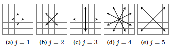
\includegraphics[keepaspectratio,width=90mm]{fdtd1.pdf}}
                \slantedcaption{Visual representation of $\bm{\nu_i}$ in each partial stencil $\Omega_i$ \parencite{Bilbao2013Constructionandoptimization}.}
                \label{fig:b1}
             \end{figure}

            The FD operator, which cancels the residuals in \ref{eq:fdtd_23}, is then applied by introducing the two-dimensional 25-point stencil
and the coefficients to be optimized:
            \begin{align} \label{eq:fdtd_24}
                D_{\Delta,\bm{\alpha},\bm{\gamma}}f(\bm{r})=\sum^5_{j=1}\alpha_j \frac{\kappa_j}{h^2}\sum^{|\Omega_j|}_{i=1}
\left(f(\bm{r}+\bm{v_i}h)-2f(\bm{r})+f(\bm{r}-\bm{v_i}h)\right),
            \end{align}
            where the position vector is $\bm{(x,z)}$, and the parameters $\bm{\alpha}\in\mathbb{R}^5$ are optimized based on the condition
            \begin{align} \label{eq:fdtd_25}
                \sum^5_{j=1}\alpha_j=1
            \end{align}
            corresponding to partial stencils divided into 5 parts from the whole 25-point stencil $\Omega\subset\mathbb{R}^2,\ \Omega=\sum^5_{i=1}\Omega_i$.
            Vector elements (for instance in \ref{eq:fdtd_24}) included in each partial stencil may be expressed with 2D Cartesian basis vectors $\bm{e_x},\bm{e_y}$,
            \begin{align} \label{eq:fdtd_26}
                \Omega_1 &=& \left[ \bm{e_x}, \bm{e_z} \right],\nonumber \\
                \Omega_2 &=& \left[ \bm{e_x}\pm\bm{e_z} \right],\nonumber \\
                \Omega_3 &=& 2\Omega_1, \nonumber \\
                \Omega_4 &=& \left[ 2\bm{e_x}\pm\bm{e_z}, \bm{e_x}\pm2\bm{e_z} \right], \nonumber \\
                \Omega_5 &=& 2\Omega_2
            \end{align}
            and
            \begin{align} \label{eq:fdtd_27}
                \kappa_j = \frac{2}{|\Omega_j| ||\bm{v}||^2},
            \end{align}
            where $|\Omega_j|$ is the index of the vector and $||\bm{v}||^2$ is the second-order norm (Euclidean norm) of any $\bm{v}_i \in \Omega_j$.

            \ref{fig:b1} shows the visual representation of the partial stencils. One finally uses $\bm{\Upsilon}=[\Omega_1,\Omega_2,\Omega_3,\Omega_4,\Omega_5]$.
            The optimized parameters $\bm{\alpha}$ are obtained by minimizing the relative phase velocity for the wave vector.
            More details may be found in \cite{Walstijn2008Onthenumerical} and \cite{Bilbao2013Constructionandoptimization}.
            \ref{fig:b2} shows the drawing of stencils of each of the FDTD schemes that we consider. Only the stencils for the $x$ direction are shown, except for the optimized FDTD scheme, which is 2D by design
and thus cannot be split into independent 1D components.
            \begin{figure}[htbp]
                    \centerline{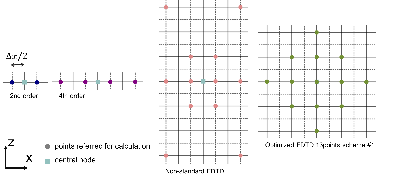
\includegraphics[keepaspectratio,width=150mm]{fdtd2.pdf}}
                \slantedcaption{Stencils for each of the FD schemes that we consider. The function value at the central node is calculated from the values at points represented by the circular
symbols. Only the stencils for the $x$ direction are shown, except for the optimized FDTD scheme, which is 2D by design
and thus cannot be split into independent 1D components.}
                \label{fig:b2}
             \end{figure}

\noindent
        \underline{\textbf{Compact schemes}}

             The main idea of compact FD schemes is to consider the calculation of FD-approximated spatial derivatives in 1D obtained by solving a 2D linear system, and then
obtain the spatial derivatives of not only one point but also its adjacent point at the same time. Here is the general derivation taken from \cite{Hixon2000Prefactoredsmallstencil} for the 1D case:
            \begin{align} \label{eq:fdtd_28}
                [B]\left[D\right]=\frac{1}{\Delta x}[C][f],
            \end{align}
            where $D$ is a 1D matrix that includes spatial derivatives of function $f$, and $B$ is a 2D matrix of coefficients. $C$ is also a 2D matrix of
coefficients. The expansion of \ref{eq:fdtd_28} at point $i$ at eighth order is then
            \begin{align} \label{eq:fdtd_29}
                \gamma(D_{i+2}+D_{i-2})+\beta(D_{i+1}+D_{i-1})+(1-\gamma-\beta)D_i\\
                = \frac{1}{\Delta x}\left[ \varphi(f_{i+2}+f_{i-2})+\eta(f_{i+1}+f_{i-1}) \right].
            \end{align}
            When gamma and beta are both zero, this becomes the equation for an explicit scheme. The spatial derivatives are then obtained:
            \begin{align} \label{eq:fdtd_30}
                [D]=[B]^{-1}\frac{1}{\Delta x}[C][f].
            \end{align}
            In \cite{Hixon2000Prefactoredsmallstencil}, $D$ is split in two parts in order to change the $B$ matrix from tridiagonal to bidiagonal for
fourth and sixth-order schemes. This scheme was initially developed for aeroacoustics but has also been successfully applied to linear wave propagation phenomena
\parencite{Rona2017Optimisedprefactoredcompact}.

    \subsection{Time domain Finite-Element Method and Spectral-Element Method}
    \label{ssec:sem}

        In order to distinguish from the case of static problems (e.g. a small deformation problem of solid mechanics), finite element methods when applied to dynamic problems
are sometimes referred to as Finite-Element Time-Domain methods (FETD or TDFE).
        The main difference between FETDs and the Spectral-Element Method (SEM) will be recalled below; it is mostly the fact that Gauss-Lobatto-Legendre points will be used,
while Gauss points are used in classical FETDs.
In other words, the SEM uses higher-order basis functions and a modified formulation that leads to a perfectly diagonal mass matrix, thus trying to combine the geometrical
flexibility of classical finite-element methods with the high accuracy of pseudospectral methods.
        Spectral methods are a class of discretization for differential equations, whose theory was for instance detailed by
\textcite{Gottlieb1977Numericalanalysisof}, and then in the 1980s spectral methods began to be applied for problems involving complex domains or media.
The SEM itself was introduced for computational fluid dynamics by \textcite{Patera1984Aspectralelement}, and later became very successful and widely used to
model the propagation of seismic wave in seismology \citep{KoTr99,Fic10,Peter2011Forwardandadjoint}
because the SEM can handle complex shapes of model boundaries in the simulated domain and also may
accurately compute surface waves. In addition, the SEM can easily model the anisotropy of a propagation medium \parencite{Komatitsch2000Simulationofanisotropic} as well as
fluid-solid boundaries \parencite{Komatitsch2000Wavepropagationnear}.

\clearpage
\noindent
        \underline{\textbf{Finite-element discretization}}

            In a finite-element discretization, a domain $\Omega$ is divided into a set of non-overlapping elements $\Omega_{e}$ as
            \begin{align} \label{eq:sem_1}
                \Omega\approx\hat{\Omega}=\sum_{e}\Omega_e.
            \end{align}
            Similarly, the boundary of $\Omega$ is also divided as
            \begin{align} \label{eq:sem_2}
                \Gamma\approx\hat{\Gamma}=\sum_{e}\Gamma_e
            \end{align}
            A differential equation is discretized based on the FEM or SEM schemes in the general form
            \begin{align} \label{eq:sem_3}
                \Biggl\{ \begin{matrix}
                    &Lu-f=0\,\,\,     &in\,\,\Omega , \\
                    &u=u_\Gamma\,\,\, &on\,\,\Gamma ,
                \end{matrix}
            \end{align}
            where $L$ is a positive definite differential operator (this assumption is required in order to fulfill the Lax-Milgram theorem, which is necessary
for converting these equations to a weak formulation), $u$ is some physical quantity (e.g. displacement etc.) and $f$ is a given function.
            For example in the acoustic wave case, from Equation \ref{eq:1_32} the corresponding equation is
            \begin{align} \label{eq:sem_4}
                \frac{1}{\rho}\nabla^2\chi-\frac{1}{\lambda}\ddot{\chi}=0.
            \end{align}

            It is generally not possible to obtain the exact solutions of second-order partial differential equations such as Equations \ref{eq:sem_3} or
\ref{eq:sem_4}. The finite-element discretization scheme adopts the so-called weighted residual formulation to solve these equations in an approximate way.
The general form obtained is then
            \begin{align} \label{eq:sem_5}
                (Lu-f,w)_W=0,
            \end{align}
            where $\forall u\in U\,(=L^2(\Omega))$ is called a trial function and $\forall w\in W\,(=L^2(\Omega))$ a test function (here $L^2$ means the $L^p$
space or Lebesgue space with $p=2$).
This inner product in Equation \ref{eq:sem_5} is a projection on the space of the test function $W$.
            This product may be written as
            \begin{align} \label{eq:sem_6}
                \int_{\Omega}(Lu-f)wd\Omega=0.
            \end{align}
            Based on this formulation, the condition \ref{eq:sem_3} needs to be satisfied in a domain $\Omega$ instead of in every defined point of $Lu-f$.

            To obtain a discretized formulation, the trial function is discretized by choosing a suitable subspace $U^h\subset U$ and its basis function $\varphi_i\, (i=0,1,\cdots,N)$,
            \begin{align} \label{eq:sem_7}
                u^h=\sum_{i=0}^Nc_i\varphi_i.
            \end{align}
            Then, using this approximated solution, \ref{eq:sem_3} is discretized as
            \begin{align} \label{eq:sem_8}
                L^hu^h-f=r^h,
            \end{align}
            where $r^h$ in $\Omega$ is called the residual of the equation. The goal of the weight residual
formulation is to determine $c_i$ by finding a solution that makes $(r^h,w)_W$ be equal to zero, i.e.,
            \begin{align} \label{eq:sem_9}
                (L^hu^h-f,w^h)_W=0,
            \end{align}
            with the reduced space of test function $\forall w^h\in W^h\subset W$, where the $W^h = \{ \psi_j\}_{i=0}^N\,;\,\psi_j\,(j=0,1,\cdots,N)$ is the basis.
By substituting them into \ref{eq:sem_6}, the discretized weighted residual formulation becomes
            \begin{align} \label{eq:sem_10}
                \sum_{i=0}^Nc_i\int_{\Omega}(L^h\varphi_i)\psi_jd\Omega=\int_{\Omega}f\psi_jd\Omega\,;\,\,i,j=0,1,\cdots,N.
            \end{align}
            Thus, the problem comes down to finding $c_i$ that fulfill Equation \ref{eq:sem_10}.

\noindent
        \underline{\textbf{Weak form}}

            From the definition of the $L^2$ inner product of Equations \ref{eq:sem_5} and \ref{eq:sem_6}, the acoustic wave equation \ref{eq:sem_4} may be
rewritten as
            \begin{align} \label{eq:sem_11}
                \int_{\Omega}\frac{1}{\rho}(\nabla^2\chi)wd\Omega=\int_\Omega\frac{1}{\lambda}\ddot{\chi}wd\Omega.
            \end{align}
            Integrating by parts and using the Green first identity on this term, Equation \ref{eq:sem_11} may be written as
            \begin{align} \label{eq:sem_12}
                -\int_{\Omega}\frac{1}{\rho}\nabla\chi\cdot\nabla wd\Omega + \int_\Gamma (\nabla\chi\cdot\bm{n})wd\Gamma
=\int_\Omega\frac{1}{\lambda}\ddot{\chi}wd\Omega,
            \end{align}
            where $\Gamma$ is the boundary of the domain $\Omega$ and $\bm{n}$ is a unit outward normal vector along $\Gamma$.

            This formulation is referred to as the weak form, while the differential form above is called the strong form.
From the Lax-Milgram theorem it is known that the equations in strong form and weak form have the same unique solution.

\noindent
        \underline{\textbf{Polynomial approximations}}

            In the formulation of the finite-element discretization, there are two parts where a polynomial approximation is applied. The first one is used
to define the shape functions that map an element in the real physical domain to the corresponding one in a reference domain.
The second is for the representation of a function (for instance describing the unknowns) inside the finite elements.

\noindent
        \underline{\textbf{Mapping}}

            Every integration term is calculated after mapping from a real domain to a reference domain. This mapping (or affine transformation) is defined for
each element depending on its shape in the real physical domain. In finite-element schemes, a shape function $N_a$ is
defined in a reference domain on each node by using a $n_l$-th order Lagrange polynomial
            \begin{align} \label{eq:sem_13}
                l_\alpha^{n_l}(\xi)=\prod_{0\leq j\leq n_l;  j\neq \alpha} \frac{\xi-\xi_j}{\xi_\alpha-\xi_j}, \,\,\,\,
l_\alpha^{n_l}(\xi_\beta)=\delta_{\alpha\beta},
            \end{align}
            where $a$ indicates the node index (i.e., the index of a given anchor point) out of a total of $n_a$ geometrical anchor nodes,
$\bm{\xi}$ is a position vector in a reference domain, and $\delta$ denotes the Kronecker delta symbol, which is equal to 1 when $i = j$ and to 0 otherwise.
            The function at an arbitrary position $\bm{\xi}$ may be calculated by interpolating from the values at the nodes by using
            \begin{align} \label{eq:sem_14}
                \bm{\xi}=\sum_{a=1}^{n_a} N_a \bm{\xi}_a.
            \end{align}
            For example in the 2D case,
            $\bm{\xi}=\bm{\xi}(\xi,\eta)$ and $\bm{\xi}_a=\bm{\xi}(\xi_a,\eta_a)$, the two parameters being in the ranges $(-1\leq \xi \leq 1,\, -1\leq \eta \leq 1)$.
            Generally for the definition of the geometrical shape functions in a TDFEM or in a SEM, it is not necessary to use high-order polynomials to define the shape function.
A degree $n_l=1\, or\,2$ is classically used.
When $n_l=2$, the corresponding number of control nodes (anchor nodes) is then 9 in a 2D quadrangular element case and 27 in a 3D hexahedral element case.
It is 4 and 8, respectively, when $n_l=1$.
            In that case of $n_l=1$, $l_0^2(\xi)=(1-\xi)/2$, $l_1^1(\xi)=(1+\xi)/2$, and when $n_l=2$, $l_0^2(\xi)=\xi(\xi-1)/2$, $l_1^2(\xi)=1-\xi^2$ and
$l_2^2(\xi)=\xi(\xi+1)/2$.
            The shape functions are defined as a product of these polynomials, for example in two-dimensional and $n_l=1$ case:
$N_1(\xi,\eta)=l_0^1(\xi)l_0^1(\eta)$, $N_2(\xi,\eta)=l_1^1(\xi)l_0^1(\eta)$, $N_3(\xi,\eta)=l_1^1(\xi)l_1^1(\eta)$ and $N_4(\xi,\eta)=l_0^1(\xi)l_1^1(\eta)$.
            The transformation from the real physical domain to the reference domain may then be expressed as $\int f(\bm{x})d\bm{x}= \int f(\bm{\xi})Jd\bm{\xi}$,
where $f$ is a function defined on the elements, $\bm{x}$ is the position vector in the real domain, and $J$ is the determinant of the Jacobian transformation, which is defined as
            \begin{align} \label{eq:sem_15}
                J=\biggl| \frac{\partial (x,y)} {\partial(\xi,\eta)}\biggl|\,\,\, \text{in 2D}, \,\,\,\,\,\, J=\biggl|\frac{\partial (x,y,z)}
{\partial(\xi,\eta,\zeta)}\biggr|\,\,\, \text{in 3D},
            \end{align}
            where $x,y,z$ are the coordinates in the physical domain. The derivatives of $\bm{\xi}$ may be calculated by
            \begin{align} \label{eq:sem_16}
                \nabla \bm{\xi} = \sum_{a=1}^{n_a} (\nabla N_a)\bm{\xi}_a.
            \end{align}

\noindent
        \underline{\textbf{Polynomial representation of functions on elements}}

            In differential pseudospectral methods as well as in variational spectral-element methods, the functions are approximated based on orthogonal polynomials as in Equation
\ref{eq:sem_7}. Different options exist for the selection of the orthogonal polynomials to be used. Here we use the Gauss-Lobatto-Legendre formulation that
is traditionally used in SEM techniques, and in particular in the SPECFEM software package that I will use in this thesis.
            The definition of the set of orthogonal polynomials based on a polynomial $P_n(x)$ of degree $n$ is
            \begin{align} \label{eq:sem_17}
                \int_{-1}^1 P_n(x)P_m(x)d\mu(x)=\int_{-1}^1w(x)P_n(x)P_m(x)dx=0,\,\,\, \text{if}\,\, m\neq n,
            \end{align}
            where $\mu$ is the Lebesgue measure. When $w(x)=1$, $P_n(x)$ is referred to as a Legendre polynomial.
            By using this Legendre polynomial, the Gaussian quadrature (or Gaussian integration)
            \begin{align} \label{eq:sem_18}
               \int_{-1}^1 f(x)d\mu(x)=\int_{-1}^1 f(x)dx=\sum_{i=0}^n w_i f(x_i)\,\,\, \text{for all}\,\, f\in \mathbb{P}_{2n+1},
            \end{align}
            is obtained for an arbitrary function $f$ of degree $2n+1$, $q,\,r$ of degree $n$ and the relation $f=q_{n+1}P_{n+1}(x)+r$, which leads to
            \begin{align} \label{eq:sem_19}
               \int_{-1}^1 f(x)dx = \int_{-1}^1 q(x) P_{n+1}(x) dx + \int_{-1}^1 r(x)dx = \sum_1^N w_i f(x_i).
            \end{align}
            This type of Gaussian integral is well known in the context of finite elements,
but roots corresponding to the collocation points are not defined at the end points of the discretization interval
(i.e. $x=-1\text{ and }1$ are \textit{not} Gauss points), which may create problems for instance to enforce boundary conditions.
By generalizing this Gaussian integration, using the supplemental definition $q(x)=P_{N+1}+aP_N+bP_{N-1}$ ($a$ and $b$ are determined
from the boundary condition $q(-1)=q(1)=0$), one obtains the roots $x_0=-1$, $x_N=1$, which are referred to as Gauss-Lobatto-Legendre points
(or, more generally, Gauss-Lobatto integration for any choice of $w(x)$), which include both end points +1 and -1.

            The roots (i.e. the Gauss-Lobatto-Legendre points) are obtained by numerically solving
            \begin{align} \label{eq:sem_20}
                (1-x^2)P'_n(x)=0,
            \end{align}
            where $P'_n$ denotes the derivative of the Legendre polynomial (i.e. $\frac{d}{dx}P_n(x)$). The weights $w_i$ are
            \begin{align} \label{eq:sem_21}
                w_i=\frac{2}{n(n+1)}\frac{1}{P_n(x_i)},\,\,\,\,\,\,\,i=0,1,\cdots,n.
            \end{align}
            The Legendre polynomial $P_n(x)$ may be derived from the singular Sturm-Liouville problem
            \begin{align} \label{eq:sem_22}
                \frac{d}{dx}((1-x^2)P'_n(x))+n(n+1)P_n(x)=0.
            \end{align}
            When the Legendre polynomials is normalized as $P_n(1)=1$,
            \begin{align} \label{eq:sem_22_a}
                P_n(x)=\frac{1}{2^n}\sum_{l=0}^{n/2}(-1)^l \Biggl( \begin{matrix}k \\ l \end{matrix}\Biggr)  \Biggl( \begin{matrix}2k-2l \\ k \end{matrix}
\Biggr) x^{k-2l}.
            \end{align}
            The recursion relation for these polynomials is
            \begin{align} \label{eq:sem_23}
                P_{n+1}(x)=\frac{2n+1}{n+1}xP_n(x)-\frac{n}{n+1}P_{n-1}(x),\,\,\,\,\,\,\,P_0(x)=1,\,\,P_1(x)=x.
            \end{align}
            Detailed explanations about such Gauss-type polynomials can be found in \textcite{Davis1984Methodsofnumerical} and \textcite{Canuto2011Spectralmethods}.
            In the spectral-element method, functions on a given spectral element are approximated by the Lagrange polynomial defined by Equation \ref{eq:sem_13}
with Gauss-Lobatto-Legendre (GLL) points (Equation \ref{eq:sem_20}).

            A function value at $\bm{\xi}(\xi,\eta,\zeta)$ in the reference domain may be expressed based on Lagrange polynomials as
            \begin{align} \label{eq:sem_25}
                f(\bm{\xi})\approx \sum_{\alpha,\beta,\gamma = 0}^{n_l} f^{\alpha\beta\gamma}l_\alpha(\xi)l_\beta(\eta)l_\gamma(\zeta),
            \end{align}
            where $f^{\alpha\beta\gamma}$ is a function value at the nodes $\alpha,\beta,\gamma$, and $l_\alpha$ is the Lagrange polynomial of $n_l$ degrees.
            The gradient of a function $\nabla f=\frac{\partial f}{\partial x}\hat{\bm{x}}_1+ \frac{\partial f}{\partial y}\hat{\bm{x}}_2+ \frac{\partial f}{\partial z}\hat{\bm{x}}_3$ is then
            \begin{align} \label{eq:sem_26}
                \nabla f(\bm{\xi}) &=       \sum_{i=1}^3 \hat{\bm{x}}_i \partial_i f(\bm{\xi})\nonumber \\
                                   &\approx \sum_{i=1}^3 \hat{\bm{x}}_i \sum_{\alpha,\beta,\gamma=0}^{n_l} f^{\alpha\beta\gamma}[
                                       l'_\alpha(\xi)l_\beta(\eta)l_\gamma(\zeta)\partial_i\xi
                                      +l_\alpha(\xi)l'_\beta(\eta)l_\gamma(\zeta)\partial_i\eta
                                      +l_\alpha(\xi)l_\beta(\eta)l'_\gamma(\zeta)\partial_i\zeta],
            \end{align}
            where a prime denotes differentiation, and $\hat{\bm{x}}_i$ is a basis vector.

\noindent
            The integration over a given element $\Omega_e$ may be discretized as
            \begin{align} \label{eq:sem_27}
                \int_{\Omega_e} f(\bm{x})d^3\bm{x} &= \int_{-1}^1\int_{-1}^1\int_{-1}^1 f(\bm{\xi}(\xi,\eta,\zeta))J(\xi,\eta,\zeta)d\xi d\eta d\zeta \nonumber
\\
                & \approx \sum_{\alpha,\beta,\gamma}^{n_l} w_\alpha w_\beta w_\gamma f^{\alpha\beta\gamma}J^{\alpha\beta\gamma},
            \end{align}
            where $w_\alpha,\,\, \alpha=0,1, \cdots,n_l$ is the weight at a given Gauss-Lobatto-Legendre point,
and $J^{\alpha\beta\gamma}=J(\xi_\alpha,\eta_\beta,\zeta_\gamma)$.

            By applying this polynomial approximation, the acoustic wave equation in the weak form \ref{eq:sem_12} for each element $\Omega_e$ and its
surrounding boundary $\Gamma_e$ is discretized as
            \begin{align} \label{eq:sem_28}
                \int_{\Omega_e}\frac{1}{\rho}\nabla\chi\cdot\nabla wd\Omega =
                \int_{-1}^1\int_{-1}^1\int_{-1}^1 \frac{1}{\rho(\bm{\xi})}\nabla\chi(\bm{\xi})\cdot \nabla w(\bm{\xi})J(\bm{\xi})d^3 \bm{\xi},
            \end{align}
            where, $w(\bm{\xi})$ is the test function. For the SEM, one chooses
            \begin{align} \label{eq:sem_29}
                w(\bm{\xi})\approx \sum_{\alpha,\beta,\gamma = 0}^{n_l} w^{\alpha\beta\gamma}l_\alpha(\xi)l_\beta(\eta)l_\gamma(\zeta).
            \end{align}
            On the right-hand side of Equation \ref{eq:sem_28}, $\nabla\chi(\bm{\xi})$ and $\nabla w(\bm{\xi})$ are discretized using Equation \ref{eq:sem_26} as
            \begin{align} \label{eq:sem_30}
                \nabla\chi(\bm{\xi}) \approx \sum_{i=1}^3 \hat{\bm{x}}_i \sum_{\alpha,\beta,\gamma=0}^{n_l} \chi^{\alpha\beta\gamma}[
                    l'_\alpha(\xi)l_\beta(\eta)l_\gamma(\zeta)\partial_i\xi
                   +l_\alpha(\xi)l'_\beta(\eta)l_\gamma(\zeta)\partial_i\eta
                   +l_\alpha(\xi)l_\beta(\eta)l'_\gamma(\zeta)\partial_i\zeta],
            \end{align}
            \begin{align} \label{eq:sem_31}
                \nabla w(\bm{\xi}) \approx \sum_{i=1}^3 \hat{\bm{x}}_i \sum_{\alpha,\beta,\gamma=0}^{n_l} w^{\alpha\beta\gamma}[
                    l'_\alpha(\xi)l_\beta(\eta)l_\gamma(\zeta)\partial_i\xi
                   +l_\alpha(\xi)l'_\beta(\eta)l_\gamma(\zeta)\partial_i\eta
                   +l_\alpha(\xi)l_\beta(\eta)l'_\gamma(\zeta)\partial_i\zeta],
            \end{align}
            and then finally the first term of the acoustic wave equation in the weak form is discretized as
            \begin{align} \label{eq:sem_32}
                & \int_{\Omega_e}\frac{1}{\rho}\nabla\chi\cdot\nabla wd\Omega \nonumber \\
                \approx & \sum_{\alpha,\beta,\gamma} w_{\alpha} w_{\beta} w_{\gamma} J^{\alpha\beta\gamma} \frac{1}{\rho^{\alpha\beta\gamma}}
                \sum_{i,j=1}^{3} \hat{\bm{x}}_i \cdot \hat{\bm{x}}_j \nonumber \\
                & \sum_{\alpha^\star,\beta^\star,\gamma^\star} \chi^{\alpha^\star\beta^\star\gamma^\star}[
                    l'_{\alpha^\star}(\xi_{\alpha}) l_{\beta^\star}(\eta_{\beta}) l_{\gamma^\star}(\zeta_{\gamma})\partial_i\xi
                   + l_{\alpha^\star}(\xi_{\alpha})l'_{\beta^\star}(\eta_{\beta}) l_{\gamma^\star}(\zeta_{\gamma})\partial_i\eta
                   + l_{\alpha^\star}(\xi_{\alpha}) l_{\beta^\star}(\eta_{\beta})l'_{\gamma^\star}(\zeta_{\gamma})\partial_i\zeta] \nonumber  \\
                & \sum_{\alpha^\diamond,\beta^\diamond,\gamma^\diamond} \omega^{\alpha^\diamond\beta^\diamond\gamma^\diamond}[
                    l'_{\alpha^\diamond}(\xi_{\alpha}) l_{\beta^\diamond}(\eta_{\beta}) l_{\gamma^\diamond}(\zeta_{\gamma})\partial_j\xi
                   + l_{\alpha^\diamond}(\xi_{\alpha})l'_{\beta^\diamond}(\eta_{\beta}) l_{\gamma^\diamond}(\zeta_{\gamma})\partial_j\eta
                   + l_{\alpha^\diamond}(\xi_{\alpha}) l_{\beta^\diamond}(\eta_{\beta})l'_{\gamma^\diamond}(\zeta_{\gamma})\partial_j\zeta] \nonumber  \\
                = & \sum_{\alpha,\beta,\gamma} w_{\alpha} w_{\beta} w_{\gamma} J^{\alpha\beta\gamma} \frac{1}{\rho^{\alpha\beta\gamma}}
                \sum_{i=1}^{3} \nonumber \\
                &\bigg[\sum_{\alpha^\star}\chi^{\alpha^\star\beta\gamma}l'_{\alpha^\star}(\xi_{\alpha})  \partial_i\xi +
                  \sum_{\beta^\star} \chi^{\alpha\beta^\star\gamma}l'_{\beta^\star} (\eta_{\beta})  \partial_i\eta +
                  \sum_{\gamma^\star}\chi^{\alpha\beta\gamma^\star}l'_{\gamma^\star}(\zeta_{\gamma})\partial_i\zeta\bigg] \nonumber \\
                &\bigg[\sum_{\alpha^\star}\omega^{\alpha^\star\beta\gamma}l'_{\alpha^\star}(\xi_{\alpha})  \partial_i\xi +
                  \sum_{\beta^\star} \omega^{\alpha\beta^\star\gamma}l'_{\beta^\star} (\eta_{\beta})  \partial_i\eta +
                  \sum_{\gamma^\star}\omega^{\alpha\beta\gamma^\star}l'_{\gamma^\star}(\zeta_{\gamma})\partial_i\zeta\bigg] \, .
            \end{align}
            The second term of the acoustic wave equation \ref{eq:sem_12} for each element $\Gamma_e$ may be discretized as (for example, for the surface where $\bm{n}=(0,0,1)$)
            \begin{align} \label{eq:sem_33}
                &\int_{\Gamma_e} (\nabla\chi\cdot\bm{n})wd\Gamma
                \approx
                \sum_{\alpha,\beta}w_{\alpha}w_{\beta}w^{\alpha\beta n_l}J^{\alpha\beta}
                \sum_{i=1}^3 \hat{\bm{x}}_i \cdot \bm{n} \nonumber \\
                &\sum_{\alpha^\star,\beta^\star}\chi^{\alpha^\star \beta^\star n_l} [
                   l'_{\alpha^\star}(\xi_{\alpha}) l_{\beta^\star} (\eta_{\beta}) l_{n_l} (\zeta_{n_l})\partial_i\xi
                + l_{\alpha^\star} (\xi_{\alpha}) l'_{\beta^\star}(\eta_{\beta}) l_{n_l} (\zeta_{n_l})\partial_i\eta
                + l_{\alpha^\star} (\xi_{\alpha}) l_{\beta^\star} (\eta_{\beta}) l'_{n_l}(\zeta_{n_l})\partial_i\zeta] \nonumber \\
                =& \sum_{\alpha,\beta}w_{\alpha}w_{\beta}w^{\alpha\beta n_l}J^{\alpha\beta}
                \bigg(\sum_{\alpha^\star}\chi^{\alpha^\star \beta n_l}l'_{\alpha^\star}(\xi_{\alpha}) \partial_3\xi+
                      \sum_{\beta^\star} \chi^{\alpha \beta^\star n_l}l'_{\beta^\star} (\eta_{\beta}) \partial_3\eta+
                                         \chi^{\alpha \beta n_l}l'_{n_l}      (\zeta_{n_l}) \partial_3\zeta\bigg).
            \end{align}
            Finally, the third term of \ref{eq:sem_12} is discretized as
            \begin{align} \label{eq:sem_34}
                \int_{\Omega_e}\frac{1}{\lambda}\ddot{\chi}wd\Omega \approx
                \sum_{\alpha,\beta,\gamma} w_{\alpha} w_{\beta} w_{\gamma} J^{\alpha\beta\gamma}
                \frac{1}{\lambda^{\alpha\beta\gamma}}w^{\alpha\beta\gamma}\ddot{\chi}^{\alpha\beta\gamma}.
            \end{align}

\noindent
        \underline{\textbf{Temporal discretization}}

            The spatially-discretized formulation may be written in matrix form as
            \begin{align} \label{eq:sem_35}
                M\ddot{\chi}_{n}+C\dot{\chi}_{n}+K\chi_{n}=F_{n},
            \end{align}
            where $M$ is the mass matrix, $C$ is the damping matrix (for instance to represent viscous damping), $K$ is the stiffness matrix,
and $F$ is force source vector at time step $n$.
In a classical explicit SEM,
one of the possible choices for time discretization is the explicit, second-order, conditionally-stable Newmark method, which links the acoustic potential values at
adjacent time steps $t=n$ and $t=n+1$ \citep{Hug87} by:
            \begin{align} \label{eq:sem_36}
                \Bigl( M+\frac{1}{2}\Delta t C \Bigr)\ddot{\chi}_{n+1} = F_{n+1}-C\Bigl( \dot{\chi}_n+\frac{\Delta t}{2}\ddot{\chi}_n\Bigr)-K\Bigl(
\chi_n+\Delta t \dot{\chi}_n+\frac{\Delta t^2}{2}\ddot{\chi}_n\Bigr)
            \end{align}
            The summations of potential terms in the brackets $\hat{\dot{\chi}}_{n+1}=\dot{\chi}_n + \frac{\Delta t}{2} \ddot{\chi}_n$ and $\hat{\chi}_{n+1} =
\chi_{n}+ \Delta t \dot{\chi}_n + \frac{\Delta t^2}{2}\ddot{\chi}_n$ are called predictors.

            \begin{figure}[htbp]
                 \centerline{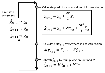
\includegraphics[width=10cm]{newmarkb.pdf}}
                \slantedcaption{Newmark-beta explicit time stepping scheme, as detailed for instance in \cite{Hug87}.}
                \label{fig:newmarkb}
            \end{figure}
%
            Figure \ref{fig:newmarkb} shows a diagram of a classical implementation of the Newmark explicit time scheme,
which is the implementation that is used in the SPECFEM software package that I will use in this thesis. At the beginning of each time step, the predictors are calculated from the
values of the potential at the previous time step. $M\ddot{\chi}_{n+1}$ is then obtained based on the sum of the stiffness term and of the force source term.
Finally, the value of $\hat{\dot{\chi}}_{n+1}$ is obtained
by multiplying the inverse of the mass matrix $M^{-1}$, which is pre-computed and stored at the initialization step of the entire simulation.
As in the SEM the mass matrix is perfectly diagonal, by construction of the SEM technique, that mass matrix is in fact a vector (i.e., only the diagonal of the mass matrix is non zero
and thus needs to be stored), and inverting it is straightforward, since the matrix is diagonal. Its inverse is thus also a simple vector.


\section{Supercomputers, High-Performance Computing (HPC), and the SPECFEM software package}

\subsection{Supercomputers and High-Performance Computing (HPC)}

Imaging what is inaccessible to direct observation, i.e. wave propagation and tomography / imaging in complex media, is a classical issue that encompasses many scientific and engineering domains, with a wide range of scientific as well as societal applications: non-destructive testing, acoustic probing, medical imaging, study of earthquake-prone regions and related seismic hazard, seismic imaging for oil and gas exploration, CO$_2$ storage and sequestration, geothermic energy... The key idea in these different imaging problems is to make use of the interactions of acoustic waves with the heterogeneities of the medium that they travel in to detect and characterize these heterogeneities. In order to address these different challenges, a necessary tool is high-performance computing (HPC) in order to be able to successfully achieve these calculations for real applications. Indeed, simulation has nowadays become the so-called third pillar of science, together with theory and experimentation, being critical for advancing our understanding of complex natural systems such as the oceans, the Earth, the atmosphere, and even the human body. Numerical modeling of acoustic wave propagation has a long history dating from the 1970s, but until a decade ago was reserved to computer experts with expensive dedicated equipment; it is now easily accessible to both academic and industrial laboratories. The success of the Partnership for Advanced Computing in Europe (PRACE) of the European Union has shown this very clearly, and the Horizon2020 program puts even more emphasis on that. Quoting the President of the European Union Jean-Claude Juncker, "mega data and high-performance computing favor economic growth as well as innovation and benefit all economic sectors as well as society as a whole, for science, research and sharing of knowledge". High-performance computing and big data are now converging, and the next big challenge we as a society are facing can be seen as High Performance Data Analytics (HPDA).

The first supercomputers appeared in the 1960s. What the word supercomputer stands for varies over time, because the most powerful computers in the world
at one point in time tend to be matched, and then surpassed, by other, more recent machines with sometimes different technology over the years.
The first supercomputers were simple single-processor computers.
In the 1970s, most supercomputers adopted a vector processor, which decoded an instruction once and applied it to a series of operands.
It was only towards the end of the 1980s that the technique of massively parallel systems was adopted, with the use of thousands of processors in the same supercomputer.

Currently, supercomputers are most often designed as unique models by traditional computer builders. Supercomputers are used for all tasks that require very high computing power, such as weather forecast, climate studies, modeling of chemical molecules, physical simulations (aerodynamic simulations, material resistance calculations,
simulation of nuclear weapon explosion, study of nuclear fusion, etc.), cryptanalysis, or simulations in finance and insurance.
Civil and military research institutions are among the largest users of supercomputers.
In France, these machines are found in national computational centers, such as the Grand \'Equipement National de Calcul Intensif (GENCI),
the Institut du d\'eveloppement et des ressources en informatique scientifique (IDRIS), the Centre informatique national de l'enseignement sup\'erieur (CINES),
the Tr\`es Grand Centre de Calcul (TGCC), the Commissariat \`a l'\'energie atomique et aux \'energies alternatives (CEA),
and also some large companies like Total, EDF or M\'et\'eo-France.

Nowadays, these computers are capable of processing and communicating very large volumes of data in a very short time.
Their design must ensure that this data can be read, transferred and stored quickly. If that were not the case, the computing power of the processors would be under-used (bottleneck).
The memory architecture of the supercomputers is thus studied and carefully optimized to continuously supply the data to each processor in order to make the most of its computing power.

Figure~\ref{fig:top500} shows that so-called petaflops supercomputers, i.e., parallel computers capable of calculating $10^{15}$ floating-point operations per second (see Table~\ref{table:petaflop_exaflop}), which are the current state-of-the-art technology\footnote{The speed of the current fastest supercomputer (as of February 2018) being about 93 petaflops, but supercomputers around 1 petaflops being more widely available.}, have become standard and easily available around 2018 (blue line), and that around 2020 the first exascale/exaflops machine (i.e., 1000 times faster than petaflops) will appear somewhere in the world (orange line). Even more importantly, it shows that it takes about nine years, from 2008 to 2017, for petaflop supercomputing to go from the largest machine in the world to something relatively easily available; thus the same will happen for exascale computing, which should therefore be easily available around 2029 or so. We are thus confident that the calculation techniques that we will develop in Chapter~4 of this thesis based on (currently) expensive 3D calculations on a large parallel computer will become standard in the future, because the machines to use them will become widely available.

    \begin{table}
        \centering
        \slantedcaption{The different standard names used for the speed of current and future supercomputers, illustrating their capacity (computational speed) in terms of the total number of floating-point operations they can compute in one second. Past names, in increasing order of speed, were: megaflop ($10^{6}$), gigaflop ($10^{9}$), teraflop ($10^{12}$).}
\vspace{5truemm}
        \begin{tabular}{lll}
        Name & Number of floating-point & Date of that technology \\
             & operations per second    &  \\ \hline
petaflop  & $10^{15}$ & current, since 2009 \\
exaflop   & $10^{18}$ & around 2020 \\
zettaflop & $10^{21}$ & around 2030? \\
yottaflop & $10^{24}$ & around 2040??
        \end{tabular}
        \label{table:petaflop_exaflop}
    \end{table}

\noindent
As mentioned by \cite{GrSt15} in their review article on the evolution of HPC, the future of high-performance computing is now being expressed and analyzed both from the point of view of how it will be implemented from a technological point of view and, more importantly, of the ways in which it will impact large fields in science and technology, commerce, industry, security and society. The trend of having increasingly more powerful supercomputers each year should continue, because in the past years, intra-node parallelism on high-performance computers has continuously been increasing, either because of the increasing number of processor cores available on CPUs, or because of accelerating computing units such as GPU graphics cards (GPU computing) or Intel accelerators (Intel Xeon Phi, Intel Many Integrated Core Architecture "Knights Landing" i.e. MIC KNL). This trend is particularly reflected in the latest TOP500 list that ranks the 500 fastest supercomputers in the world, in which the first two supercomputers are heterogeneous systems equipped with accelerators. In order to fully benefit from this hardware evolution, software packages and computing applications often require substantial modifications. Exascale machines will start to appear around 2020; with such machines, 3D calculations for wave propagation in complex nuclear reactor core models, as introduced in this thesis, will become something routinely used.

In this thesis, we will mostly use the French national OCCIGEN / GENCI (Grand \'Equipement National de Calcul Intensif) machine located at CINES (Centre Informatique National de l'Enseignement Sup\'erieur) in Montpellier, France. It is a parallel supercomputer built by the BULL Atos company that comprises 4212 Intel processors of the Haswell and Broadwell types with a total of 85824 processor cores, and a total of 283 terabytes of memory, with a peak processing speed of 3.5 petaflop per second. As of February 2018 it is the 54th largest supercomputer in the world.


    \subsection{The SPECFEM software package: A very efficient numerical code for acoustic or seismic wave propagation simulation}

SPECFEM is an open-source software package that can model acoustic or seismic wave propagation in complex media, using the spectral-element method.
The first versions of this codes were developed by Dimitri Komatitsch and Jean-Pierre Vilotte at Institut de Physique du Globe (IPGP) in Paris,
France from 1995 to 1997 and then by Dimitri Komatitsch and Jeroen Tromp at Harvard University and Caltech, USA for seismic wave propagation simulation.
It has more recently been applied to ultrasonic non-destructive testing and to ocean acoustics.
The code is being developed on Github (\url{http://github.com/geodynamics}), which is a development platform for open-source projects.
It is also available on the Computational Infrastructure for Geodynamics (CIG) platform, which is widely used in Earth Sciences.
2D, 2.5D (axisymmetric, \cite{Bottero2016Anaxisymmetrictime}) and 3D versions of the package are available.
The software package simulates acoustic or seismic wave propagation
at the local or regional scale and performs full waveform imaging (FWI) or adjoint tomography based upon the spectral-element method
(SEM).

            \begin{figure}[htbp]
                 \centerline{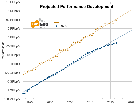
\includegraphics[width=13cm]{top500_list_evolution.pdf}}
                \slantedcaption{Speed of the fastest supercomputer in the world (in orange) and its projected evolution over the years, as well as the speed of the 500th, i.e. of a machine typical of moderate-size supercomputers easily available to researchers at regional or laboratory sites (in blue). The extrapolation is reliable, as shown by the very good fit over the first twenty years. In log scale, adapted from www.top500.org.}
                \label{fig:top500}
            \end{figure}

The SEM is a continuous Galerkin technique \citep{TrKoLi08,Peter2011Forwardandadjoint},
which can easily be made discontinuous \citep{BeMaPa94,KoWoHu02,ChCaVi03,LaWaBe05,Kop06};
it is then close to a particular case of the discontinuous Galerkin
technique \citep{ReHi73,LeRa74,HuHuRa99,RiWh03,DuKa06},
with optimized efficiency because of its tensorized basis functions
\citep{WiStBuGh10,AcKo11}. In particular, it can accurately handle very distorted mesh elements \citep{OlSe11}.
Effects due to lateral variations in compressional-wave speed, shear-wave
speed, density, and topography of object interfaces can all be included.
The package can accommodate full 21-parameter anisotropy
(see~\citet{ChTr07}) as well as lateral variations in attenuation
\citep{SaKoTr10}. Adjoint capabilities and finite-frequency kernel
simulations for imaging of unknown complex media are also included \citep{TrKoLi08,FiIgBuKe09,ViOp09,MoChKoWa15}.
In fluids, when gravity is turned off, SPECFEM3D uses the classical linearized Euler equation.
The goal in my thesis is to adapt and use this package to simulate ultrasonic wave propagation
in a sodium reactor core, for instance using approximations of such a complex propagation medium coming from thermal-hydraulic simulations
of such a core as performed by CEA using its TrioCFD software package (Figure~\ref{fig:specfem}).

        \begin{figure}[htbp]
                \centerline{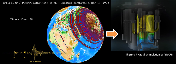
\includegraphics[width=17cm]{specfem.pdf}}
            \slantedcaption{The SPECFEM open-source software package that will be used in this thesis
was initially developed in seismology, to simulate the propagation of seismic waves propagating in the Earth following large earthquakes
(left, from the users manual of SPECFEM); the goal in this thesis is to adapt it and use it to simulate ultrasonic wave propagation
in a sodium reactor core, for instance using approximations of such a complex propagation medium coming from thermal-hydraulic simulations
of such a core as performed by CEA using its TrioCFD software package (right, from the CEA home page).}
            \label{fig:specfem}
        \end{figure}

It has very good accuracy and convergence properties \citep{Coh02,DeSe07,SeOl08,AiWa09,MeStTh12}.
The spectral element approach admits spectral rates of convergence
and allows exploiting $hp$-convergence schemes. It is also very well
suited to parallel implementation on very large supercomputers \citep{KoTsChTr03,TsKoChTr03,Peter2011Forwardandadjoint}
as well as on clusters of GPU accelerating graphics cards \citep{KoMiEr09,Komatitsch2010Highorderfinite,Kom11}.
Tensor products inside each element can be optimized to reach very
high efficiency \citep{DeFiMu02}, and mesh point and element numbering
can be optimized to reduce processor cache misses and improve cache
reuse \citep{KoLaMi08a}. The SEM can also handle triangular (in 2D)
or tetrahedral (in 3D) elements \citep{WinBoyd96,KoMaTrTaWi01,MeViSa06}
as well as mixed meshes, although with increased cost and reduced
accuracy in these elements, as in the discontinuous Galerkin method.

Figure \ref{fig:spec_flow} shows a typical workflow when simulating wave propagation in a complex model based on the SPECFEM software package.
The process is divided into four main steps: mesh creation, partitioning of the mesh created for parallel processing when running on a parallel computer,
simulation database generation, and final resolution and calculation of wave propagation (the so-called solver step).
For explicit time marching, the user can freely choose between different schemes:
second-order Newmark scheme \parencite{Newmark1959Amethodof}, fourth-order four-stage classical
Runge-Kutta \parencite{Butcher2016Numericalmethodsfor}, or fourth-order six-stage LDDRK (Low-Dissipation and low-Dispersion Runge-Kutta)
\parencite{Berland2006Lowdissipationand}. Available mesh types (in terms of geometry of the mesh elements) are 4-node and 9-node quadrangular elements
in the 2D case and 8-node and 27-node hexahedral elements in the 3D case.
For mesh creation, a simple (relatively basic) internal mesh creation tool is provided, but any external mesh creation tool that can produce hexahedral meshes can also
be used, for instance CUBIT/Trelis (developed by Sandia National Laboratories, USA) or Gmsh \parencite{Geuzaine2009Gmsh:A3}.
In the case of infinite or semi-infinite media, the code implements Convolution or
Auxiliary Differential Equation Perfectly Matched absorbing Layers
(C-PML or ADE-PML) \citep{KoMa07,Komatitsch2008Anunsplitconvolutional,MaKoGeBr10}.

\clearpage

        \begin{figure}[htbp]
            \centerline{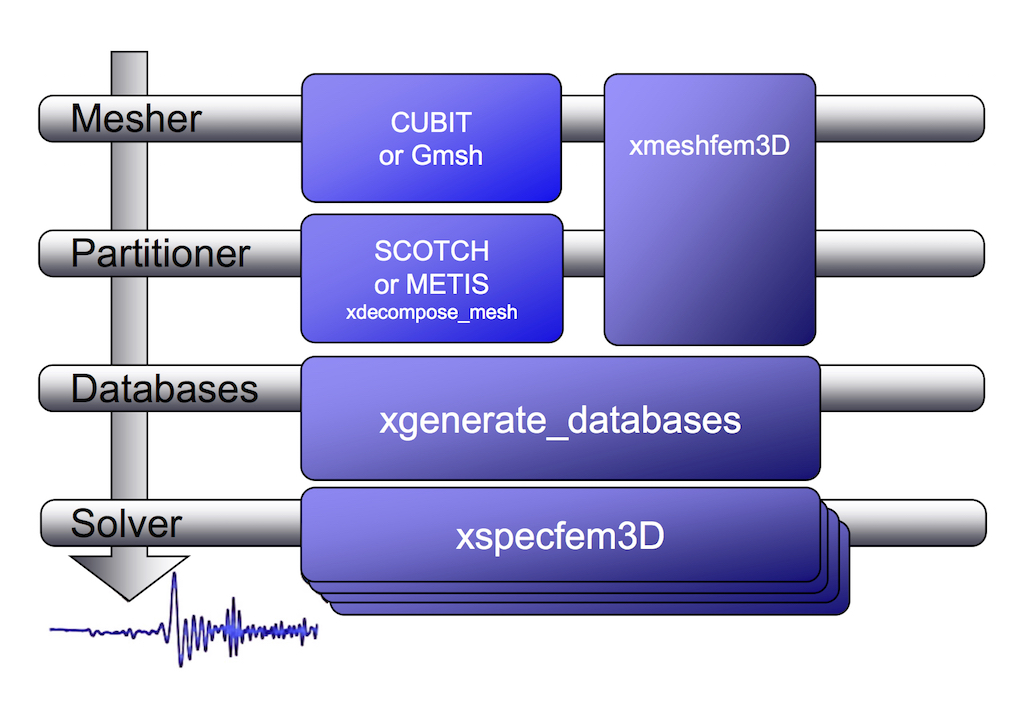
\includegraphics[width=12cm]{spec_flow.jpg}}
        \slantedcaption{Workflow of a typical wave propagation calculation when using the SPECFEM software package.
The process is divided into four main steps: mesh creation, partitioning of the mesh created for parallel processing when running on a parallel computer,
simulation database generation, and final resolution and calculation of wave propagation (the so-called solver step). Taken from the users manual of SPECFEM.}
        \label{fig:spec_flow}
        \end{figure}

The SEM was originally developed in computational fluid dynamics \citep{Patera1984Aspectralelement,MaPa89}
and has been successfully adapted to address problems in seismic wave
propagation. Early seismic wave propagation applications of the SEM,
utilizing Legendre basis functions and a perfectly diagonal mass matrix,
include \citet{CoJoTo93}, \citet{Kom97}, \citet{FaMaPaQu97},
\citet{KoVi98} and \citet{KoTr99}, whereas applications involving
Chebyshev basis functions and a non-diagonal mass matrix include \citet{SePr94}, \citet{PrCaSe94} and \citet{SePrPr95}.
In the Legendre version that we use in SPECFEM the mass matrix is purposely slightly inexact but diagonal (but can be made exact if needed, see \cite{Teu15}),
while in the Chebyshev version it is exact but non diagonal.
For a detailed introduction to the SEM as applied to regional seismic
wave propagation, one can refer to \citet{KoVi98,KoTr99,ChKoViCaVaFe07,TrKoLi08}
and even more specifically to \citet{Lee2009Effectsoftopography,LeChKoHuTr09}.
A detailed theoretical analysis of the dispersion
and stability properties of the SEM is available in \citet{Coh02}, \citet{DeSe07}, \citet{SeOl07} and \citet{MeStTh12}.

In a spectral-element method, some spurious modes, which have some similarities with classical so-called "Hourglass modes" in finite-element techniques,
although in the SEM they are not zero-energy modes, can appear in some (but not all) cases in the spectral element in which the source is located.
Fortunately, they do not propagate away from the source element.
However, this means that if you put a receiver in the same spectral element as a source, the recorded signals may in some cases be wrong, typically exhibiting some spurious
oscillations, which are often even non causal.
If that is the case, an easy option is to slightly change the mesh in the source region in order to get rid of these Hourglass-like spurious modes,
as explained in \cite{DuLiScGa14}, in which this phenomenon is described in details, and in which practical solutions to avoid it are suggested.

\clearpage

All SPECFEM software is written in Fortran2003 with full portability
in mind, and conforms strictly to the Fortran2003 standard. It uses
no obsolete or obsolescent features of Fortran. The package implements parallel
programming based upon the Message Passing Interface (MPI) \citep{GrLuSk94,Pac97}.

The code is particularly well suited to very large parallel supercomputers.
SPECFEM3D won the prestigious Gordon Bell international computer science award for best performance at the SuperComputing~2003
conference in Phoenix, Arizona (USA) \citep{KoTsChTr03}.
It was a finalist again in 2008 for a run at 0.16 petaflops (sustained) on 149,784 processors
of the `Jaguar' Cray XT5 system at Oak Ridge National Laboratories
(USA) \citep{CaKoLaTiMiLeSnTr08}. It also won the BULL Joseph Fourier supercomputing award in 2010.
It reached the sustained one petaflop performance level for the first time in February 2013
on the Blue Waters Cray supercomputer at the National Center for Supercomputing Applications (NCSA), located at the University of Illinois at Urbana-Champaign (USA).

  %%%%%%% Chapter 2: basic equations and physical description of the problem

\cleardoublepage
%
\chapter{2D simulations for a simplified upper-core model}

\label{chap:3}
\vspace*{-12mm}
{\footnotesize \sl
Section \ref{sec:2DGRF} of this chapter has been published as an article in an international journal, under the reference: Masaru Nagaso, Joseph Moysan, Sa\"{\i}d Benjeddou, Nicolas
Massacret, Marie-Aude Ploix, Dimitri Komatitsch and Christian Lhuillier, Ultrasonic thermometry simulation in a random fluctuating medium: Evidence of the
acoustic signature of a one-percent temperature difference, Ultrasonics, vol. 68, p. 61-70, doi: 10.1016/j.ultras.2016.02.011 (2016).}

\vspace*{+2mm}
    In this chapter, we will first perform a comparative study between several Finite Difference in the Time Domain (FDTD) numerical schemes and a Spectral-Element Method (SEM)
to simulate ultrasonic wave propagation in the core of a sodium reactor. From these results, we will show that
the SEM scheme has high computational stability and efficiency for our modeling purposes.
    After the experimental study of the accuracy properties of these two numerical simulation techniques,
we will perform a 2D simulation study with a Gaussian random field to introduce heterogeneity in the propagation medium.
We will analyze the effects of stochastically-generated
temperature fluctuation fields on 2D acoustic wave propagation, and the feasibility and accuracy of ultrasonic thermometry at the upper-core region of a sodium-cooled fast reactor.

    \section{Validation of the SPECFEM numerical code for our problem, and comparison with other numerical schemes}
    \label{sec:UPSILON}

\vspace*{-3mm}
        In order to gain good knowledge about features of numerical modeling methods for ultrasonic wave propagation in a sodium reactor core, let us compare the acoustic fields
calculated based on several types of full waveform modeling methods. We use the configuration of an experiment performed at CEA Cadarache and called UPSILON in order to see the effect of temperature heterogeneity on the
accuracy and stability of the numerical simulations. For these purpose, we used the numerical code SPECFEM for the SEM calculations and SEISMIC\_CPML for the FDTD
calculations.

    \subsection{SEISMIC\_CPML}

        SEISMIC\_CPML is a software package that was developed mostly by Dimitri Komatitsch and Roland Martin at CNRS. As SPECFEM,
SEISMIC\_CPML is an open-source code distributed by the Computational Infrastructure for Geodynamics (CIG, \url{http://geodynamics.org/cig/software/seismic_cpml}).
        It can solve two/three-dimensional isotropic/anisotropic acoustic/elastic and viscoelastic/poroelastic wave equation based
on finite differences in the time domain. Convolutional perfectly matched absorbing layers \citep{KoMa07} are also implemented to mimic infinite or semi-infinite propagation media.
More details about SEISMIC\_CPML can be found at \url{http://komatitsch.free.fr/README_seismic_cpml.html}
For our comparisons, we improved this code by increasing the order of spatial discretization, i.e., we increased the number of grid points that are used for the calculations
of derivatives at a given grid point. We also modified the 2D version of the code
to support parallel computing based on MPI (the 3D version of the code already had such parallel support based on MPI, but the 2D pressure version
did not). Thanks to these two improvements, we managed to simulate wave propagation for
high-frequency (\SI{2.25}{\mega\hertz}) acoustic emission, with low computational error and high stability and with significantly shorter computational time.

    \subsection{Simulation for the UPSILON experiment}

        UPSILON is an experiment that was designed to observe how an acoustic wave is affected by thermal heterogeneity in silicon oil.
This experiment has initially performed by Nicolas Massacret in his Ph.D. study at CEA/LIET \citep{Massacret2014Etudedunemethode}.
The heterogeneity of the temperature field in silicon oil is
generated by heating wires, and changes in an acoustic wave front may be observed from recorded acoustic signals using a Schlieren optical system.
Table \ref{table:upsilon_tools} shows the names and specifications of equipments used in this experiment.
        We therefore decided to model the UPSILON configuration in our acoustic wave propagation numerical simulations. The model geometry is shown in Figure \ref{fig:upsilon_conf}.
        We computed wave propagation for two states of the propagation medium, one with a homogeneous medium and the other with the same geometrical configuration but
with a heterogeneous medium. The sound velocity field is calculated based on
\begin{align} \label{eq:2_11_1}
    C_p = 1056.60 - 2.72 T_{Celcius} \, .
\end{align}

        \begin{figure}[htbp]
                \centerline{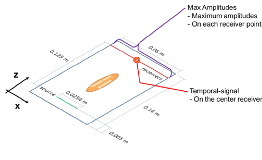
\includegraphics[width=12cm]{upsilon_conf_v2.pdf}}
            \slantedcaption{Configuration of the models for our simulations. The UPSILON experiment is modeled in two dimensions. The green line is the
source line that emits a quasi-plane wave. The elliptical part in orange is the heated area.}
            \label{fig:upsilon_conf}
        \end{figure}

The shape of the heated area and medium
temperature is defined by Equation \ref{eq:2_11} in all heterogeneous simulations.
The density of silicon oil was calculated based on the equation of sound speed for a fluid $c=\sqrt{K/\rho}$
where $c$ is sound speed, $K$ is the bulk modulus, and $\rho$ is density.
$K$ was calculated from the known density value of silicon oil from its specification sheet: \SI{970}{\kilo\gram\per\cubic\metre}.
An acoustic emission surface is modeled as a line source (represented by the green line in Figure
\ref{fig:upsilon_conf}) composed of many individual point sources placed on a straight line. A Ricker time wavelet (i.e., the second derivative of a Gaussian)
is emitted from all these source points, and a Hamming window
function is applied to the amplitude of each emission depending on the distance of that source to the central point of the line source in order to emit a
quasi-plane wave:
        \begin{align} \label{eq:2_11}
            T(x,z)=20.00+8.00e^{-5.00*10^4(x-0.03)}\frac{1}{1+e^{400(z-0.08)}}\frac{1}{1+e^{400(-z+0.08)}}.
        \end{align}

        \begin{table}
            \slantedcaption{Names and specifications of the different equipments used in the UPSILON experiment by \cite{Massacret2014Etudedunemethode}.}
\vspace{5truemm}
            \makebox[1 \textwidth][c]{
            \resizebox{1. \textwidth}{!}{
            \begin{tabularx}{\textwidth}{llll}
                \hline
                Name & Manufacturer & Product & Others \\ \hline
                Silicon oil & Carl Roth Silicon Oil & M 10,000 cSt & \parbox[t]{4cm}{density at 20$\degree$:\\\num{970} - \num{980} \si{kg/m^3}} \\
                \parbox[t]{2cm}{Acoustic probe\\(emitter)}  & Olympus Panametrics & \parbox[t]{4cm}{Standard Contact Video Scan,\\V104-RB} &
\parbox[t]{4cm}{Mono-element,\\frequency 2.25 MHz,\\surface diameter \SI{3.175}{\centi\meter}} \\
                \parbox[t]{2cm}{needle\\hydrophone\\(receiver)} & No data & No data & \parbox[t]{4cm}{bandwidth 1-10 MHz}\\ \hline
            \end{tabularx}
            }
            }
            \label{table:upsilon_tools}
        \end{table}

            Figure \ref{fig:upsilon_geo} shows the experimental configuration of UPSILON. The formulation for sound velocity \ref{eq:2_11_1} is an empirical formula
that was experimentally established by \cite{Massacret2014Etudedunemethode}. The ultrasonic emitter at \SI{2.25}{\mega\hertz} has a diameter of 1 inch (i.e. \SI{2.54}{\centi\meter}),
and the profile of the acoustic field is measured using a quarter-inch plane receiver at \SI{2.25}{\mega\hertz} to obtain a fine measurement.
            Thermocouples are used to measure temperature in the area of interest, and a polynomial variation is used to describe the distribution of temperature.
This polynomial expression was then simplified using the symmetric formula of Equation~\ref{eq:2_11} in order to make simulations easier to perform.
            This experiment was efficient to illustrate the phenomena that were looked for: deviation of ultrasounds by temperature gradients, and wave speed variations.
To our knowledge it was the first demonstration that ultrasonic measurement techniques are accurate enough to detect thermal-hydraulic effects on wave propagation.
The originality of this experiment was to create a localized and stable temperature gradient thanks to the thermal silicon oil properties.

    \begin{figure}[htbp]
            \centerline{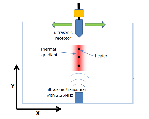
\includegraphics[width=12cm]{upsilon_geo.pdf}}
            \slantedcaption{Experimental configuration of UPSILON, taken from \cite{Massacret2014Etudedunemethode}.}
        \label{fig:upsilon_geo}
    \end{figure}


    \subsection{Results of the comparisons between the different numerical schemes}

We compared results obtained with the SEM technique with those obtained based on the standard FDTD, Optimized-FDTD, and NSFDTD schemes presented in the previous chapter.
        First, we performed convergence tests for both homogeneous and heterogeneous cases of all schemes by changing the number of grid points per
wavelength in the case of FDTD, or the number of spectral elements per wavelength in the case of the SEM. In the FDTD tests, 10, 20, 25, 30, 35, 40 points per wavelength were tested.

Excellent convergence for this very sensitive (and thus very difficult) test was obtained with 40 points per wavelength
for Optimized-FDTD and NSFDTD, but second/fourth order FDTD could not achieve convergence even with
40 nodes per wavelength in the homogeneous case.
For the SEM, we tested 1, 2, 4, 6 elements per wavelength and achieved excellent convergence with 4 or 6 elements per wavelength.
        We compared all schemes based on two criteria: maximum amplitude values recorded at each receiver point on the receiver line indicated as the orange
line in Figure \ref{fig:upsilon_conf}, and the single signal recorded at the center of the receiver line.

        Figure \ref{fig:upsilon_res1} of upper row shows the results of comparison between all schemes for the homogeneous simulation, and Figure \ref{fig:upsilon_res1} of lower row shows the
results for the heterogeneous case. In the homogeneous results, SEM (SPECFEM2D), optimized-FDTD and NSFDTD converge to extremely similar results,
while the signals of second/fourth-order FDTD still exhibit dispersion of the signal peaks i.e. they have not yet fully converged.
Because this configuration of acoustic emission involves very high frequency
waves, it requires very high resolution for the spatial discretization, and this is why second/fourth-order spatial orders based on classical schemes
are not sufficient for this numerical experiment, considering also the very large total number of time steps involved, i.e. the cumulative numerical dispersion involved.

On the other hand, it is clear that the SEM reaches convergence with a smaller
number of grid points than the other schemes, which is directly linked to the reduction of the required amount of computational resources (in the SEM,
spectral elements with fourth-order polynomial basis functions have 4 computation nodes for each element, thus 6 elements per wavelength is approximately equivalent to 24 grid points
per wavelength). This means that the required number of grid points for convergence of the SEM calculation is 24 (nodes for SEM) / 40 (nodes for FDTD) \string^ 2 (the number of spatial dimensions) * 100 (\%) = \SI{36}{\percent} of the number of nodes required for FDTD in the two-dimensional case;
in the three-dimensional case, only 24/40 \string^ 3 (number of spatial dimensions) * 100(\%) = \SI{21.6}{\percent} of the nodes required for 3D FDTD are necessary for convergence of the 3D SEM calculation.

\noindent
        In the heterogeneous results in Figure \ref{fig:upsilon_res1} at the lower row, the curve of second-order FDTD is not shown because its calculation did not converge.
Again, the fourth-order FDTD results exhibit numerical errors appearing for instance as dispersion of the peaks. Each temporal signal has two peaks
while the homogeneous case has only one peak. This is because the direct wave which passed through the center of the heated medium was significantly slowed down.
Instead, the wave that traveled through colder regions of the medium arrives at the central receiver faster by going around the hot spot, and the slowed direct
wave arrives later, which explains why the second peak has a larger value than the first.
        The curves obtained based on all the other schemes (on the right-hand side of the figure) are all very close,
however we still find some differences between the curves of the max amplitude (on the left-hand side of the figure),
which comes from the fact that the maximum amplitude curve is very sensitive to the change of shape of the wave front.

        We calculated the correlation coefficients between SEM and other method for homogeneous and heterogeneous case. To do so, we used the temporal signals recorded at the
center of the receiver line. The results are shown in Table \ref{table:upsilon_res3}. It is clear that for both the homogeneous and heterogeneous cases that NSFDTD
and optimized-FDTD have higher correlation coefficients than the two more classical but less accurate methods.

        \begin{figure}[htbp]
                \centerline{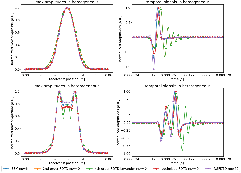
\includegraphics[width=\textwidth]{upsilon_res.pdf}}
            \slantedcaption{Comparison between SEM, 2nd/4th-order FDTD, Optimized-FDTD, NSFDTD in the homogeneous case (upper row) and in the heterogeneous case (lower row).}
            \label{fig:upsilon_res1}
        \end{figure}

        \begin{table}
            \centering
            \slantedcaption{Correlation coefficients between SPECFEM and different FDTD schemes. The temporal signal of each scheme at the center of the receiver
line is used for this comparison.}
\vspace{5truemm}
            \begin{tabular}{lll}
                \toprule
                Computation scheme & Homogeneous & Heterogeneous \\ \midrule
                Second-order FDTD     & \num{4.22143e-1} & Did not converge \\
                Fourth-order FDTD     & \num{4.22105e-1} & \num{4.57660e-1}   \\
                NSFDTD             & \num{9.53819e-1} & \num{9.54614e-1}   \\
                Optimized-FDTD     & \num{9.54240e-1} & \num{9.52261e-1}   \\ \bottomrule
            \end{tabular}
            \label{table:upsilon_res3}
        \end{table}

In future work, Massacret's Upsilon experiment should be improved by using a 2D matrix transducer in order to be able to perform a 3D comparison between experiments and modeling.
This discussion of such future work will be continued in the Conclusions and perspective chapter (\autoref{chap:5}).
We can conclude that the SEM has advantages not only because of its capacity to model curved geometrical surfaces thanks to
the finite-element discretization scheme involved, but also thanks to its capacity to achieve convergence with smaller computational resources.
Let us mention that in the calculations based on SPECFEM, we used a very accurate Low-dissipation and low-dispersion Runge-Kutta (LDDRK) time scheme \citep{Berland2006Lowdissipationand}
for time marching, while for FDTDs we used a standard Newmark scheme \citep{Hug87}.
This difference thus favors the SEM results when a large number of time steps is involved.

\section{Ultrasonic thermometry simulation in a random fluctuating medium: Evidence of the acoustic signature of a one-percent temperature difference}
\label{sec:2DGRF}

Let us now study the development potential of ultrasonic thermometry in a liquid fluctuating sodium environment similar to that present in a Sodium-cooled Fast
Reactor, and thus investigate if and how ultrasonic thermometry could be used to monitor the sodium flow at the outlet of the reactor core. In particular we
study if small temperature variations in the sodium flow of e.g. about \SI{1}{\percent} of the sodium temperature, i.e., about 5\textdegree{}C, can have a
reliably-measurable acoustic signature. Since to our knowledge no experimental setups are available for such a study, and considering the practical
difficulties of experimentation in sodium, we resort to a numerical technique for full wave propagation called the spectral-element method, which is a highly
accurate finite-element method owing to the high-degree basis functions it uses. We obtain clear time-of-flight variations in the case of a small temperature
difference of one percent in the case of a static temperature gradient as well as in the presence of a random fluctuation of the temperature field in the
turbulent flow. The numerical simulations underline the potential of ultrasonic thermometry in such a context.

    \subsection{Positioning of the problem}

        Our work aims at studying potential improvements upon temperature sensors currently used for sodium temperature measurements, such as thermocouples, by resorting to
ultrasonic thermometry. Ultrasonic thermometry can be implemented based on several approaches. A first one consists of using an ultrasonic thermometer: by
sending an ultrasonic pulse through a thin rod with acoustic discontinuities such as notches or sudden diameter changes, and measuring the time between the
initial pulse and the reflections of that pulse, the rod is segmented into a multi-point temperature sensor \parencite{Daw2002Ultrasonicthermometryfor}. For
our study however, the starting point regarding thermometry for in-service temperature measurement at the outlet of the core is a second approach described in
a 1985 British patent registered by A. McKnight et al. entitled "Remote temperature measurement" \parencite{McKnight1987Remotetemperaturemeasurement}. The
main idea in that patent is to use an ultrasonic beam that impinges on the two diametrically opposite edges of a subassembly separated by a known distance.
Measuring the time interval between the two echoes (and knowing the relation between celerity and temperature) then allows one to deduce the mean temperature
of the liquid sodium between these two points.

        However, since several parameters can influence the time-of-flight measurement, several challenging issues need to be addressed in order for such a
technique to be usable in practice. The liquid sodium exiting the core of a nuclear reactor is a turbulent flow with thermal heterogeneities, and local flow
variations can thus influence wave propagation. The shape of the reflected echoes, which depends on the fuel assembly geometry, can also be of importance and
should be taken into account in the signal processing method used. In some particular cases, the proportion of gas micro-bubbles can also vary and modify the
relation between celerity and temperature. Recent work has specifically focused on these aspects of wave propagation in a turbulent medium
\parencite{Massacret2014Modellingofultrasonic} as well as evaluation of gas proportion in an SFR \parencite{Cavaro2011Microbubblecloudcharacterization}.

        In this study our goal is to study the development potential of ultrasonic thermometry in liquid sodium and thus to investigate if and how ultrasonic
thermometry could be used to monitor the outlet of a sodium reactor core. In particular we want to see if small temperature variations (of e.g. about
\SI{1}{\percent} of the sodium temperature, i.e., about 5\textdegree{}C) in the sodium flow could have a reliably-measurable acoustic signature. The gas
proportion is considered as constant in our study and flow rate is also neglected. Since to our knowledge no operating experimental setups would allow us to
obtain a precise description of the fluctuating medium, and considering the practical difficulties related to experimentation in sodium, we will turn to
highly-accurate numerical modeling based on a full wave modeling technique.

        One of the difficulties in order to get a good model is to define what a liquid-sodium fluctuating medium can be. Its temperature and flow velocity
field fluctuate by the interaction of a flow and the core structure composed of various assemblies, and they also fluctuate due to the thermo-dynamical
equilibrium of the medium.
To the best of our knowledge, no Computational Fluid Dynamics code can accurately generate such media at reasonable cost at a scale
compatible with the ultrasonic scale that we want to target. We will thus turn to physical modeling to generate the fluctuating medium.
In general, physical characteristics of a heterogeneous liquid medium fluctuate spatially and temporally, depending on its nature and on the environment.
Such a heterogeneity is quite complex to model in a deterministic way because of many uncontrolled factors and thus it is common to model them based on a stochastic process.
This issue has been addressed in the literature regarding modeling of heterogeneous liquid sodium in the context of wave propagation simulation.

        In order to verify the possibility of measuring a small temperature variation in such an environment, which is the main goal of our study, it is
necessary to consider the effect of temperature fluctuations caused by turbulent flow. For this purpose, we regard the temperature field as a combination of a
static temperature distribution, which is to be measured, and a fluctuation part. Considering that fluctuating part, we resort to the Gaussian random field
method, which is a random field generator based on a spectral method introduced by \textcite{Shinozuka1972Digitalsimulationof}.

        The section will be structured as follows: In \autoref{ssec:2dgrf_the} we will describe the thermometry concept at the outlet of the fuel assembly. In \autoref{ssec:2dgrf_num} we will describe the configurations defined for our simulations and the definition of the temperature fields. We will then discuss the results and show that our 2D numerical simulations underline the potential of ultrasonic thermometry in \autoref{ssec:2dgrf_res}.

    \subsection{Thermometry at the outlet of nuclear fuel assemblies} \label{ssec:2dgrf_the}
        Current setups for thermal instrumentation above a reactor core consist of hundreds of thermocouples assembled in thermo-wells, one above each fuel
assembly that needs to be monitored. However, as indicated above, there is a need for developing more efficient instrumentation for the next generation of
nuclear reactors. One important issue to address is the ability to perform faster measurements, as the expected response time of the complete temperature
instrumentation in these future reactors is 0.1 s or even less instead of at best about 1 s with sheathed thermocouples. Another interest for the ultrasonic
method is that it is less sensitive to sodium jet bending than thermocouples. Additional improvements could consist of reducing the number of electrical wires
located above the reactor core, which would open new design possibilities.

      Acoustic thermometry based on ultrasonic transducers is a good candidate for such improved monitoring, as such transducers are already under development
for instance at French Atomic Commission for various local measurements performed during maintenance operations. For in-service monitoring however, temperature
and sodium flow characteristics are not the same as during maintenance operations (temperature is significantly higher, and sodium is flowing instead of idle),
but transducers are designed for very high-temperature (up to 600 \textdegree{}C or even more) and should thus still be suitable for that usage.

        Acoustic thermometry is based on the dependence of ultrasonic wave celerity on temperature in a given medium.
\textcite{Sobolev2011Databaseofthermophysical} has established the following empirical relationship between temperature and wave celerity in sodium:
        \begin{align}\label{eq:3_1}
            c_p\, [\text{m}\, \text{s}^{-1}] = 2723-0.531\cdot T\,[\text{kelvin}].
        \end{align}
        where $c_p$ is the celerity of ultrasonic waves in meters per second and $T$ is sodium temperature in Kelvin degrees.
        Density is also temperature dependent \parencite{Sobolev2011Databaseofthermophysical}:
        \begin{align}\label{eq:3_2}
            \rho\,[ \text{kg} \, \text{m}^{-3} ]=1014-0.235\cdot T\,[ \text{kelvin} ].
        \end{align}
        The 1985 patent mentioned above considered the use of an ultrasonic beam as the basic tool for monitoring. As the celerity of ultrasonic waves is about
2300 m/s in sodium at 550\textdegree{}C and as the distance between the monitored sub-assemblies and the transducer in future reactor designs should typically
vary between a few tens of centimeters and several meters, using ultrasounds should indeed make measurement with a short response time possible because the
time-of-flight will be in the range of milliseconds. The actual response time of an ultrasonic measurement device would then mainly be due to signal processing
time in that device. Furthermore, with a single transducer operating at grazing incidence it would then be possible to simultaneously measure the temperature
of the sodium flow at the outlet of several fuel sub-assemblies, allowing for the use of a smaller total number of measurement devices in the reactor.

        Our goal in this section is to investigate how to develop a method involving the propagation of an ultrasonic beam towards two surfaces separated by
known distance, which will both generate echoes. As mentioned in the 1985 patent the edges of the fuel subassembly heads are good candidates for generating the
echoes, i.e., for being these two surfaces. The model to design for such a study must take into account the fact that in-service thermal-hydraulic conditions
above the reactor core may disturb the propagation of ultrasonic waves between the ultrasonic transducer and the subassembly heads in terms of time delay as
well as deflection. There are indeed several sources of thermal heterogeneities above the core: the temperature difference between sodium flowing out of two
neighboring sub-assemblies can reach values as high as 50\textdegree{}C owing to the design of the core; Moreover, the sodium that flows in the spaces located
between the sub-assemblies as well as the sodium that flows out of the spaces left clear for insertion of control rods or safety devices is cooler by several
tens of degrees than sodium flowing out of the sub-assemblies. Ultrasonic waves will therefore propagate in a medium in which temperature is significantly
heterogeneous.

        In addition, the flow above the core is turbulent, with local flow speeds of about 3 m/s, and speed gradients are about several meters per second per
centimeter. The presence of such a turbulent field has an impact on the propagation of ultrasonic waves. This phenomenon is used in acoustic flow-meters to
measure the flow speed (\cite{Liu2011Thecalculationof} and \cite{Weber2004Ultrasonicbeampropagation}). In the case of acoustic thermometry this could lead to
errors in the estimation of temperature if that effect is not properly taken into account.

        In spite of these difficulties, operating solutions have been developed in the past for instance in the French Phenix reactor using the so-called
"SONAR" device, not for thermometry but rather for telemetry \parencite{Berton1996Continuousmonitoringof}. In that device the transducer was designed to
measure a specular reflection from a small facet of about 3 $\text{cm}^2$ machined on the fuel assembly head. Signal-to-noise ratio was about + 23 dB in a
nominal situation.

        Since we want to investigate if diffraction echoes could be used for thermometry or telemetry in a sodium reactor core, let us design a 2D ultrasonic
propagation model suitable for such a medium and with suitable instrumentation to simulate the propagation of ultrasonic waves. Since we are going to resort to
plane wave sources, 2D simulations are a good and significantly less expensive approximation and it is not necessary to resort to 3D calculations. Performing
such simulations will enable us to quantify the disturbance caused by the thermal-hydraulic characteristics of sodium and to determine if they could be
problematic in the context of acoustic thermometry.

        Figure \ref{fig:ult1} describes the 2D geometry that we consider. We model a transducer source (S) using a line of acoustic point sources of width w. We
define a setup with grazing incidence of about 7\textdegree{} because measurements performed in water in previous work gave good experimental results in such a
configuration \parencite{Tenchine2010Somethermalhydraulic}. The solid (stainless steel) tube representing the fuel assembly has an inner diameter d of 100 mm.
The thickness e of the tube is 13 mm. Echoes will arrive from edges E1 and E2, and possibly from edges E1' and E2' as well. We will measure time differences
between the main echoes E1 and E2.
        \begin{figure}[htbp]
            \centerline{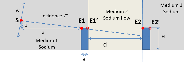
\includegraphics[width=12cm]{ult1.pdf}}
            \slantedcaption{Ultrasonic thermometry configuration used in our study.}
            \label{fig:ult1}
        \end{figure}


    \subsection{Numerical simulations} \label{ssec:2dgrf_num}

        \underline{\textbf{Modeling of the propagation medium}}

            We consider the framework of an effective medium to model the propagation medium. Density and wave velocity of the background model are modified to
incorporate the effects of a heterogeneous medium due to the sodium flow, which only implies temperature gradients.
As mentioned by \cite{Godin2002Aneffectivequiescent},
three conditions have to be met to validate the first hypothesis, which is that of linear behavior, as well as the second hypothesis,
which is that of plane (or quasi-plane) wave propagation. These conditions are that:
\vspace*{-4mm}
            \begin{itemize}
                \item the deviation of the beam must remain weak,
                \item the gradient of the flow velocity relative to the Mach number must remain moderate,
                \item the typical size of the heterogeneities must be large compared to the acoustic wavelength.
            \end{itemize}
\vspace*{-4mm}
            These three conditions were verified and shown to apply in the cases under study in another study based on a ray-tracing code
\parencite{Massacret2014Modellingofultrasonic} and on the analysis of real thermal-hydraulic data \parencite{Tenchine2010Somethermalhydraulic}. Characteristic
sizes of flow heterogeneities, typically ranging between 0.1 cm and 10.0 cm, are also large compared to the wavelengths of the ultrasonic waves considered
\parencite{Grewal1982Watersimulationof}.

            As the measurement area is located just above the outlet of the fuel assembly, the flow is relatively regular and with smooth variations only and
high Reynolds number. In such a case ultrasonic wave propagation is mainly affected by temperature distribution in the flow, and in our study we can therefore
neglect the effects of the speed of the flow. The assumption of an effective medium is thus valid and the propagation medium can then simply be described by
its density and the bulk modulus of the fluid, without having to explicitly model the fluid flow.

            The study of the PLAJEST experiment of mixing cold and hot sodium flows \parencite{Kimura2007Experimentalinvestigationon}, and its detailed
numerical simulation at the French Atomic Commission using the TrioU code \parencite{Brillant2004Largeeddysimulation} leads us to choose a continuous parabolic
variation of temperature inside the jet. Regarding the possible presence of micro-bubbles, there are not enough data for future reactors to currently be able
to take this parameter into account. Doing so will require a complete study, as the influence of the presence of such micro-bubbles will depend on bubble sizes
as well as on transducer frequency \parencite{Cavaro2011Microbubblecloudcharacterization}. The relation between ultrasonic velocity and temperature is given by
equation \ref{eq:3_1}, and equation \ref{eq:3_2} gives the density of sodium as a function of temperature T in Kelvin.

            In order to perform our spectral-element simulations, we first create a mesh of the structure under study using the 'Gmsh' mesh creation tool
\parencite{Geuzaine2009Gmsh:A3}. The mesh created is entirely composed of quadrangles, as required by the spectral-element technique. Around the region of
interest we resort to an absorbing boundary layer called the Perfectly Matched Layer (PML, \cite{Komatitsch2008Anunsplitconvolutional}) in order to efficiently
absorb the outgoing wave field; we use three layers of spectral elements on the outer edges of the mesh in order to implement it. The computational domain has
a size of 723 mm (width) by 156 mm (height) and contains 448,704 elements. We use a polynomial degree N = 4 to define the basis functions in the
spectral-element method, thus each spectral element contains (N + 1)2 = 25 grid points and the total number of unique grid points is 7,108,112. Considering the
sound velocity in liquid sodium at 450\textdegree{}C (2339 m/s) and a dominant frequency of the ultrasonic source of 1 MHz, the number of grid points per
shortest wavelength in the medium is thus approximately 4.7. We simulate a total physical time of 202.5 $\mu$s using a time discretization step of $7.5 \times
10^{-9} \text{s}$, i.e., a total of 27,000 time steps.

            To speed up the calculations we resort to parallel computing on a cluster of computers \parencite{Peter2011Forwardandadjoint}. Once the mesh is
created we thus partition it according to the number of processor cores to be used for the calculation. Each processor core then carries out the calculations
in a sub-domain, and the results are recombined at the end of each time step of the time-stepping algorithm. We perform our calculations using 128 processor
cores.

        \underline{\textbf{Geometry of the assemblies and source description}}

            We select the location to use for the ultrasonic source (S) based on the position of point E1 and on distances a and b in Figure \ref{fig:ult1}.
Values of a and b equal to 100 mm and 12 mm lead to an incidence angle of 7\textdegree{}. To simulate the behavior of the transducer and create a quasi-plane
wave of finite extension we sum 1000 point sources using a Hamming apodization function over a total width of about 67.6 mm. Each point source has a Ricker
(i.e., the second derivative of a Gaussian) wavelet time function with a dominant frequency of 1 MHz \parencite{Cristini2012Someillustrativeexamples}. The
height of the upper part of the stainless steel tube is 50 mm, its thickness is 13 mm and its inner diameter is 100~mm.
            The ratio between the known propagation distance and the time-of-flight difference between echoes E2 and E1 enables us to estimate the velocity of
sound and then, based on equation \ref{eq:3_1}, the mean temperature of the sodium flow on the outer edge of the tube.

        \underline{\textbf{Temperature variations studied}}

            As stated above the propagation medium is in a turbulent state and its temperature distribution varies in a complicated fashion both in space and
in time between, inside and above the assembly edges. \textcite{Buffet1984Studyoftemperature}, \textcite{Fiorina1998Applicationofthe} and
\textcite{Lue2012Stochasticsimulationof} have studied wave propagation in a turbulent liquid metal flow and, regarding sound velocity in such a medium, have
decomposed the medium into two parts: a heterogeneous static part, and a random fluctuation part caused by the turbulent flow.
            In our study we will first perform simulations in the presence of a static temperature distribution only, and then in a second step with
temperature fluctuations in the whole propagation region, generated based on a Gaussian random field.
            \begin{figure}[htbp]
                    \centerline{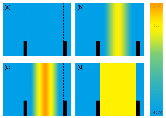
\includegraphics[width=12cm]{ult2.pdf}}
                \slantedcaption{The four types of static temperature fields that we will use in our study: (a) T450, (b) TVAR, (c) TVAR+5, (d) T500. They
differ only between the two edges of the outlet (vertical dotted lines). Model T450 has a constant temperature of 450\textdegree{}C everywhere, TVAR has a
parabolic variation from 450\textdegree{}C to 500\textdegree{}C between the two assembly edges, TVAR+5 has a parabolic variation from 450\textdegree{}C to
505\textdegree{}C, and T500 has a constant temperature of 500\textdegree{}C between the two edges and of 450\textdegree{}C outside.}
                \label{fig:ult2}
            \end{figure}

            \underline{\textbf{Static temperature fields}}

                As shown in Figure \ref{fig:ult2} we select four simple static temperature distributions in and at the outlet of the tube (called "medium 2" in
the following) as well as in the surrounding sodium (called "medium 1"). In the first temperature profile (T450) we consider a homogeneous medium with a
constant temperature of 450\textdegree{}C in both medium 1 and medium 2. It will be our reference case. In the second profile (TVAR) we consider a gradual
evolution of temperature in medium 2, using a symmetric parabolic profile varying from 450\textdegree{}C to 500\textdegree{}C between the edge and the axis of
the tube. Medium 1 still has a constant temperature of 450\textdegree{}C. In the third profile (TVAR+5) we use the same kind of profile as in the second but
with an increase of 5\textdegree{}C, i.e., about \SI{1}{\percent}, of the maximum temperature in medium 2 only. The parabolic profile thus varies from
450\textdegree{}C to 505\textdegree{}C. In the fourth profile (T500) we finally consider a simplified temperature model of 500\textdegree{}C everywhere in the
tube and at its outlet (medium 2) and 450\textdegree{}C everywhere in medium 1.
                In these four media the arrival time of the first echo does not vary, since medium 1 is unchanged. We thus focus our analysis on the variations
of the second echo (wave reflection at point E2 in Figure \ref{fig:ult1}).

            \underline{\textbf{Temperature fluctuation using a Gaussian random field}}

                Gaussian random fields have been developed for digital simulation of multivariate, multidimensional, or multivariate-multidimensional random
processes. They are used for instance in numerical analysis of nonlinear structures, numerical solution of stress wave propagation through a random medium, and
eigenvalue problems of structures that have random homogeneous properties. Here we create Gaussian random fields for the fluctuation of the temperature field
given by,
                \begin{align}\label{eq:3_4}
                    \frac{1}{T(\bm{r})}=\frac{1}{T_0}(1+\epsilon(\bm{r})),
                \end{align}
                where $T(\bm{r})$ is temperature at the spatial position $\bm{r}$, $T_0$ is given by each of the static temperature profiles defined in Figure
\ref{fig:ult2}, and $\epsilon(\bm{r})$ is the fluctuation part calculated by the Gaussian random field.
                Following work on wave propagation in turbulent media (e.g. \textcite{Lue2012Stochasticsimulationof}) we define the randomness of the
temperature fluctuation as an isotropic homogeneous random field by a series cosine functions, expressing $\epsilon(\bm{r})$ as:
                \begin{align}\label{eq:3_5}
                    \epsilon(\bm{r})=\sqrt{2}\sum_{k=1}^N \{S_{\epsilon}(\omega_k)\Delta \omega_k\}^{1/2}cos(\bm{\omega}_k \cdot \bm{r}+\phi_k),
                \end{align}
                where $k$ is the mode number and $N$ is the total number of modes. $\bm{\omega}_k$ is the wave vector, its angle from a coordinate axis of the
wave vector of each mode is $\theta_k = cos^{-1} \frac{\bm{\omega}_k}{|\bm{\omega}_k|}$, and its modulus $|\bm{\omega}_k|=\omega_k$ is defined by
$\omega_k=\omega_l + (k-1)\Delta \omega_k$, linearly distributing it in the range $[\omega_l,\omega_u]$. $\Delta \omega_k = \frac{\omega_u-\omega_l}{N-1}$ is
the wave vector increment. For this process two random input values $\theta_k$ and $\phi_k$ are necessary: $\theta_k$ is distributed uniformly and randomly in
$0\leq\theta_k<2\pi$. Hence its probability density function $Pr$ from 0 to $2\pi$ is $Pr[0\leq\theta_k<2\pi]=1/2\pi$. The other random variety $\phi_k$ is
also uniformly distributed in $0\leq\phi_k\leq 2\pi$. $S_{\epsilon}(\omega_k)$ is the spectral density function and is calculated based on the autocorrelation
function $C_{\epsilon}(r)$ as:
                \begin{align}\label{eq:3_6}
                    S_{\epsilon}(\omega_k)=\frac{1}{2\pi}\int_{-\infty}^\infty C_{\epsilon}(r)e^{-i\omega_kr}dr,
                \end{align}
                where $r$ is the magnitude of the position vector $\bm{r}$ (i.e. $r = |\bm{r}|$). For a Gaussian random field, the autocorrelation function is
defined by a Gaussian distribution following the central limit theorem:
                \begin{align}\label{eq:3_7}
                    C_{\epsilon}(r)=\sigma_{\epsilon}^2R(r)=\sigma_{\epsilon}^2e^{-(r^2/l_{\epsilon}^2)},
                \end{align}
                with $C_{\epsilon}(r)$ the covariance, $R(r)$ the autocorrelation function, $\sigma_{\epsilon}^2$ the variance of the random value, and
$l_{\epsilon}$ the characteristic length of the random pattern. $R$ is the distance between two different points $(\bm{r}_1,\bm{r}_2)$ in the region in which
the random field is simulated, i.e., $r=|\bm{r}_1-\bm{r}_2|$.

                After applying a Fourier transform to equation \ref{eq:3_6} the spectral density function then writes:
                \begin{align}\label{eq:3_8}
                    S_{\epsilon}(\omega_k)=\frac{\sigma_{\epsilon}^2}{2\pi}\int_{-\infty}^\infty e^{-(r^2/l_{\epsilon}^2)}
e^{-i\omega_kr}dr=\frac{\sigma_{\epsilon}^2l_{\epsilon} }{2\sqrt{\pi}}e^{-(\omega_k^2 l_{\epsilon}^2/4)}.
                \end{align}
                We use typical values from the NAJECO experiment \parencite{Tenchine2010Somethermalhydraulic} to choose the characteristic length $l_{\epsilon}
=$ 0.03 m. We set the standard deviation of the fluctuation to $\sigma_\epsilon =$ 0.029 to be able to generate a maximum difference of about 30 degrees
(Figure \ref{fig:ult3}), following a thermal-hydrodynamic calculation result obtained at the French Atomic Commission
\parencite{Tenchine2010Somethermalhydraulic}. The total number of modes $N$ and the range of the wave vector modulus $[\omega_l,\omega_u]$ need to be chosen
carefully: $N$ needs to be large enough to keep a sufficient data set because Equation \ref{eq:3_5} is asymptotically an exact expression for the covariance
function when $N$ tends to infinity \parencite{Shinozuka1972Digitalsimulationof}, and not doing so may introduce numerical errors
\parencite{Mantoglou1982TheTurningBands}. The range $[\omega_l,\omega_u]$ needs to be wide enough to express the entire curve of the spectral density function.
After numerical tests and following a discussion about the minimum requirements of these values in \textcite{Lee2009Effectsoftopography} we select $N$ = 64,
$\omega_u = 6/l_\epsilon$, and $\omega_j=-\omega_u$. (The range of the wave vector needs to be symmetric because the spectral density function of the Gaussian
process is symmetric).

                \begin{figure}[htbp]
                        \centerline{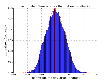
\includegraphics[width=9cm]{ult3.pdf}}
                    \slantedcaption{Distribution of the 30 different temperature fluctuation fields. The magnitude of the fluctuation is defined as the
difference with the average temperature calculated from all fluctuation fields (450\textdegree{}C).}
                    \label{fig:ult3}
                \end{figure}

                \begin{figure}[htbp]
                        \centerline{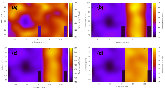
\includegraphics[width=13cm]{ult4.pdf}}
                    \slantedcaption{Examples of generated fluctuating temperature fields obtained when using the (a) T450, (b) TVAR, (c) TVAR+5 and (d) T500
temperature profiles of Figure \ref{fig:ult2}.}
                    \label{fig:ult4}
                \end{figure}

                We generate 30 different patterns of the fluctuation field, and thus obtain 30 temperature fields to be simulated by superimposing the
fluctuation field with the static temperature field based on Equation~\ref{eq:3_4}.
                Figure \ref{fig:ult3} shows the distribution of the magnitude, defined as the difference with the average temperature (450\textdegree{}C), of
the temperature fluctuation for all 30 fluctuation patterns.
                Figure \ref{fig:ult4} shows examples of such generated temperature fields. In the generation of the fluctuation field the origin point of
$\bm{r}$ (i.e., the coordinate of point $\bm{r_1}$) in Equation \ref{eq:3_4} is set at the upper-left corner of the nearest assembly edge. In Figure
\ref{fig:ult4}a the temperature scale is truncated to show the random patterns more clearly. The temperature changes in the vertical shapes along the sodium
jet are due to the temperature profile (see Figure \ref{fig:ult2}); they are right edges in the case of the rectangular profile (Figure \ref{fig:ult4}d) and
more variable edges in the case of a parabolic distribution (Figure \ref{fig:ult4}b and \ref{fig:ult4}c).

                We then carried out simulations of wave propagation in these models and calculated times of flight in the 120 resulting patterns of the
temperature field, constructed by overlaying the 30 Gaussian random field patterns with each of the four types of static temperature profile, as we will
describe in the next section.

    \subsection{Results and discussion} \label{ssec:2dgrf_res}

        \underline{\textbf{Results with static temperature fields}}

            In Figure 5 we show the pressure of the acoustic wave in the computational domain normalized between -1 (blue) and +1 (red), with color intensity
obeying a power law with exponent 0.3 in order to significantly enhance small values for visualization purposes. Such a nonlinear color scale amplifies the
real amplitude of the minor echoes such as the second diffraction E1' in order to observe them more easily. All amplitudes below \SI{1}{\percent} are discarded
in order to avoid visually amplifying very small-amplitude numerical noise. Figure \ref{fig:ult5} highlights several aspects of wave propagation near the upper
part of the fuel assembly. The waves diffracted from edges E1 and E1' are both clearly observed.
            The time $t =$ 88.125 \si{\micro\second} at which the figure is drawn allows us to observe the wave just before it interacts with the second point
E2. Since the incidence angle is very small, the lower part of the wave front goes through the thickness of the tube with a much greater velocity (about 5.8
\si{\milli\meter\per\micro\second} in steel versus about 2.3 \si{\milli\meter\per\micro\second} in sodium) and is well seen as a small wave that propagates
before the main one. Figure \ref{fig:ult5} also shows a superimposition of waves: the main wave and the wave diffracted from E1'. This illustrates the interest
of such snapshots as well as movies of wave propagation in the time domain to facilitate signal analysis and identification of wave fronts in such applications.

            \begin{figure}[htbp]
                    \centerline{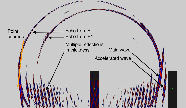
\includegraphics[width=13cm]{ult5.pdf}}
                \slantedcaption{Snapshot of wave propagation at time $t =$ \SI{88.125}{\micro\second} simulated using our spectral-element numerical modeling
technique; we display the pressure variation field (blue being negative and red positive).}
                \label{fig:ult5}
            \end{figure}
%
            Figure \ref{fig:ult6} shows the signals recorded at point S of Figure \ref{fig:ult1} for a time window that allows us to observe the signal
reflected off the second edge (point E2) for the four different temperature configurations. These signals are recorded when the waves come back to the source,
i.e. in the so-called echo mode in non-destructive testing. As wave velocity decreases when sodium temperature increases (Equation \ref{eq:3_1}), the signal is
delayed when temperature increases. The respective time delays of the four signals are qualitatively in agreement with the expected behavior: the hotter medium
2 is, the larger the delay for the time-of-flight from point E2 is as well. We observe a small time difference when the parabolic temperature distribution is
increased by 5\textdegree{}, i.e., by about one percent. The small accelerated wave observed in Figure \ref{fig:ult5} leads to a weaker signal that arrives
before the main echo around time $t =$ \SI{179}{\micro\second}. This signal is \SI{20}{\decibel} lower than the maximum signal because this part of the beam
underwent transmission through steel; in practice in a real experimental setup it could thus be masked by signal noise. Both of these signals are due to the
waves diffracted off point E2. As the duration of the wave corresponds to about two periods, similar to a highly damped transducer, no interferences occur
between these two waves; this can also be seen in Figure \ref{fig:ult5}, in which the waves are clearly separated.

            In order to perform a more quantitative analysis, in Table \ref{table:ult1} we give the arrival times in \si{\micro\second} of the second echo
measured at the signal maximum. Corresponding pressures have arbitrary units because, since the wave equation is linear, the amplitudes of the signals do not
significantly vary and thus amplitude cannot be used to detect temperature variations in this configuration; we thus analyze arrival times only in our study.
            The changes in the time-of-flight of the second echo at point E2 provide information on the ability and sensitivity of the method to detect small
temperature variations in the case of the absence of temperature fluctuation. Between Simulations 2 and 3 we find that the increase of 5\textdegree{}C of the
maximum of the temperature profile leads to a shift of \SI{68}{\nano\second}. As the time of flight of echo E1 is always the same, this difference is also the
difference between the times of flight of the echoes on the two edges ($t_{E2} - t_{E1}$). In a reactor such a time difference could be measured using a
\SI{1}{\mega\hertz} signal, i.e., a short signal, but that would require good signal-to-noise ratio and signal stability.

            \begin{figure}[htbp]
                    \centerline{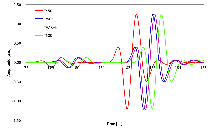
\includegraphics[width=16cm]{ult6.pdf}}
                \slantedcaption{Comparison between the echoes reflected off point E2 in the four simulations performed for the model with right-angle edges.}
                \label{fig:ult6}
            \end{figure}

            \begin{table}
                \centering
                \slantedcaption{Time-of-flight and amplitude of the echo coming back from point E2 for the four different temperature configurations in the
case of a right-angle geometry.}
\vspace{5truemm}
                \begin{tabular}{lll}
                Configuration    & \parbox[t]{5cm}{Arrival time of\\the second echo (\si{\micro\second}) $t_{E2}$} & \parbox[t]{5cm}{Maximum amplitude \\
(arbitrary units)} \\ \hline
                1. T450          & \num{182.346}                  & \num{1.24284}                   \\
                2. TVAR          & \num{183.000}                  & \num{1.24971}                   \\
                3. TVAR+5        & \num{183.068}                  & \num{1.25112}                   \\
                4. T500          & \num{183.330}                  & \num{1.24801}                   \\
                \end{tabular}
                \label{table:ult1}
            \end{table}


        \textit{\textbf{Results with temperature fluctuation}}

            \underline{\textbf{Effect of temperature fluctuation on time-of-flight}}

                Let us now study the fluctuation in times of flight when temperature fluctuations in the medium are taken into account and see if it is still
possible to detect such short time differences. We simulate wave propagation for \num{30} random temperature fields added to each of the four static fields,
leading to a total of \num{120} different propagation media, and obtain fluctuations of the time of flight for echo E2 but also for echo E1. We thus consider
that the fluctuating media introduce a random noise around the true time of flight corresponding to a static situation. Figure \ref{fig:ult7} shows the
resulting distribution of time of flight $t_{E2}$ for the four static temperature cases. We observe an overlapping of various times of flight. An averaging
procedure would be necessary to reconstruct the true time of flight as defined above. Table \ref{table:ult2} summarizes time of flight measurements for both
the E1 and E2 echoes without fluctuations (left column) and using averaged times of flight in the case of stochastic fluctuations (right column). We then
calculate the time difference between the two echoes ($t_{E2} - t_{E1}$), as this variation of the time difference would be a signature of variation in the
sodium jet. The \num{5}\textdegree{}C difference between the two parabolic profiles TVAR and TVAR+5 creates a \SI{68}{\nano\second} difference between the
times of flight difference from edges E2 and E1. This time difference is equal to about \SI{66}{\nano\second} when an average process is performed over
\num{30} fluctuating temperature field.

                \begin{figure}[htbp]
                        \centerline{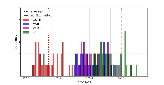
\includegraphics[width=20.5cm]{ult7.pdf}}
                    \slantedcaption{Distributions of variation of times of flight resulting from temperature fluctuations for each of the \num{120}
temperatures profiles considered, i.e. the \num{30} random profiles superimposed to each of the four static temperature profiles.}
                    \label{fig:ult7}
                \end{figure}

                \begin{table}
                    \small
                    \centering
                    \slantedcaption{Variations of time of flight between results for the cases without temperature fluctuations and averaged results from
\num{30} measurements in cases with fluctuations.}
\vspace{5truemm}
                    \begin{tabular}{lll} \hline
                                  & $t_{E2}$ without fluctuation (\si{\micro\second}) & \parbox[t]{5cm}{Averaged $t_{E2}$ from \num{30}\\measurements
(\si{\micro\second})} \\ \hline
                    T450          & \num{182.346}                  & \num{182.354}                   \\
                    TVAR          & \num{183.000}                  & \num{183.008}                   \\
                    TVAR+5        & \num{183.068}                  & \num{183.074}                   \\
                    T500          & \num{183.330}                  & \num{183.337}                   \\
                                  & $t_{E1}$ without fluctuation (\si{\micro\second}) & \parbox[t]{5cm}{Averaged $t_{E1}$ from \num{30}\\measurements
(\si{\micro\second})} \\ \cline{2-3}
                    T450          & \num{86.250}                  & \num{86.266}                   \\
                    TVAR          & \num{86.250}                  & \num{86.266}                   \\
                    TVAR+5        & \num{86.250}                  & \num{86.266}                   \\
                    T500          & \num{86.250}                  & \num{86.266}                   \\
                                  & \parbox[t]{5cm}{Time difference ($t_{E2}-t_{E1}$) without fluctuation (\si{\micro\second})} & \parbox[t]{5cm}{Time
difference\\($t_{E2}-t_{E1}$) averaged $t_{E2}$ from\\\num{30} measurements (\si{\micro\second})} \\ \cline{2-3}
                    T450          & \num{96.098}                  & \num{96.088}                   \\
                    TVAR          & \num{96.750}                  & \num{96.742}                   \\
                    TVAR+5        & \num{96.818}                  & \num{96.808}                   \\
                    T500          & \num{97.080}                  & \num{97.071}                   \\
                                  & \parbox[t]{5cm}{Variation of time difference\\$\Delta(t_{E2}-t_{E1})$ between TVAR and TVAR+5 without\\fluctuation
(\si{\micro\second})} & \parbox[t]{5cm}{Variation of time difference\\$\Delta(t_{E2}-t_{E1})$ between TVAR\\and TVAR+5 averaged from\\\num{30} measurements
(\si{\micro\second})} \\ \cline{2-3}
                    $(t_{E2}-t_{E1})_{TVAR}$          & \num{10.500}                  & \num{10.476}                   \\
                    $(t_{E2}-t_{E1})_{TVAR+5}$        & \num{10.568}                  & \num{10.542}                   \\
                    \parbox[t]{5cm}{$\Delta(t_{E2}-t_{E1})=$\\$(t_{E2}-t_{E1})_{TVAR+5}\\-(t_{E2}-t_{E1})_{TVAR}$}       & \SI{68}{\nano\second}
  & \SI{66}{\nano\second}                   \\\hline
                    \end{tabular}
                    \label{table:ult2}
                \end{table}

            \underline{\textbf{Detection of variations of statistic temperature by averaging}}

                In Figure \ref{fig:ult8} we perform a more complete statistical analysis. If we calculate the standard deviation of time-of-flight measurements
due to the random pattern in the temperature fields we can evaluate the probability of success to separate times of flight for a \SI{1}{\percent} temperature
difference, i.e., 5\textdegree{}C in our case.

In Table \ref{table:ult2} we find that the variation in the time-of-flight difference $\Delta(t_{E2}-t_{E1})$
between echoes E2 and E1 due to the \SI{1}{\percent} temperature difference is \SI{68}{\nano\second} in the case of static temperature fields; Considering
classical Gaussian statistics, it is possible to statistically separate the two time-of-flights differences $\Delta(t_{E2}-t_{E1})$ with a
\SI{68}{\percent} chance of success if the standard deviation of the time-of-flight measurements is lower than \SI{34}{\nano\second} (\num{2}$\sigma$).
To improve the chance of success the standard deviation should be lower than \SI{17}{\nano\second} (\num{4}$\sigma$) to separate times of flight with
\SI{95}{\percent} of success, and lower than \SI{11}{\nano\second} (\num{6}$\sigma$) to separate times of flight with \SIlist{99}{\percent} of
success. Figure \ref{fig:ult8} shows that these levels of confidence are reached when using respectively \num{15}, \num{24} and \num{28} measurements.

                \begin{figure}[htbp]
                        \centerline{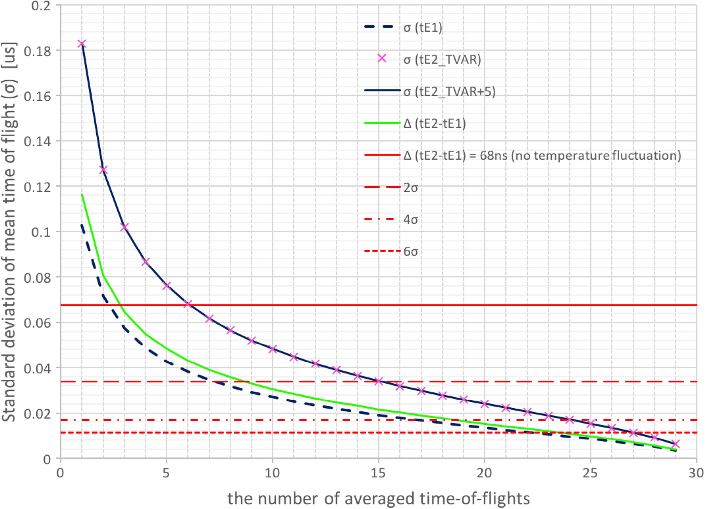
\includegraphics[width=16cm]{ult8.pdf}}
                    \slantedcaption{Variation of the standard deviation of the mean time-of-flight with respect to the number of times-of-flight used to
calculate the mean value.}
                    \label{fig:ult8}
                \end{figure}

\vspace*{-0.8truecm}
\section{Conclusions of this chapter}

In \autoref{sec:UPSILON}, we demonstrated the accuracy and efficiency of the SEM for our application, i.e. application to a heterogeneous medium (silicon oil)
using a \SI{2.25}{\mega\hertz} acoustic wave.
The results calculated with the SEM were compared with several FDTD methods, including a classic 2nd-order FDTD, a 4th-order FDTD,
and two types of more-recently developed methods, namely the optimized FDTD and Non-Standard FDTD.
Even if those recent FDTD methods showed good convergence properties, the SEM exhibited higher numerical efficiency for the problems that we want to study.

In \autoref{sec:2DGRF}, we presented a 2D numerical modeling study based on a spectral-element method in the time domain to analyze variations of time of flight due to
temperature changes in a fluid medium. We have shown that our numerical approach can accurately model the principle of ultrasonic thermometry above the core of
a Sodium Fast Reactor. Based on our numerical approach we have illustrated the sensitivity of an ultrasonic thermometry method to a relatively weak temperature
change. In the simulations with a static temperature profile we have shown that a temperature variation of about \SI{1}{\percent} of the average temperature
could be detected, as this temperature variation induces a time shift of about \SI{68}{\nano\second}.

We generated 120 patterns of temperature fields using a Gaussian random field and examined their effect on the time-of-flight of the signal reflected
off the assembly edges. We investigated the effect of temperature fluctuations on the variations of times-of-flight for four different patterns of static
temperature profiles. Under these thermodynamically and acoustically complex conditions we found that it may be difficult to detect a \num{5}-degree i.e. one
percent variation in the static temperature field based on a single measurement, but also showed that by averaging times-of-flight coming from about \num{30}
measurements such detection becomes possible with a high level of confidence.

We took the thermal static heterogeneity of the medium into account by considering a simplified medium and superimposing fluctuations created
based on a random field generator. In the next chapter of this thesis, we will extend our simulations to take into account a more realistic medium defined
using computational fluid dynamics results for new reactor designs that are currently
being performed in a project called ASTRID (Advanced Sodium Technological Reactor for Industrial Demonstration) \parencite{Coz2011Sodiumcooledfast}.
Taking flow rates i.e. a moving fluid into account will require further development of our spectral-element technique in future work. In addition to using a more complete
description of liquid sodium above the fuel assemblies, further studies should also focus on better understanding the origin of signal noise to understand
which part could be produced by medium fluctuations such as eddies or vortices. The results that we have obtained can be useful for ultrasonic thermometry, but
our conclusions should also be valid for telemetry applications in which time-of-flight measurements are used to accurately locate objects in a liquid medium.

The study in this section relied on the hypothesis that the temperature field in the region near the outlet may be described by superimposing a static
field and a fluctuation field. The static field was provided as simple profiles, for instance having a parabolic shape. The fluctuation fields were generated
using a Gaussian random field.
However, at the moment, the Gaussian random field method is only validated for fields without strong flows,
and thus we are still not sure to what extent a Gaussian random field hypothesis is applicable for regions in which flows with strong variations may exist.
It is expected that Gaussian random fields are applicable to simulate regions that are located sufficiently far from the outlets of the sodium flow,
but less applicable in regions located closer to the outlets. Hence, in future studies, it will be necessary to examine the applicability of a Gaussian random field
approximation to represent medium fluctuations, depending on the distance from the sodium outlets, by comparing the results obtained based on wave propagation in a medium
represented by a Gaussian random field to those coming from a computational fluid dynamics (CFD) simulation.

  %%%%%%% Chapter 3: SEISMIC_CPML + 2D results of the article with Said

\cleardoublepage
%\chapter{3D simulation of acoustic wave propagation with a realistic temperature field}

\section{Objective of the study in this chapter}

In the previous chapter, we studied wave propagation in liquid sodium with temperature heterogeneity (\autoref{sec:UPSILON}).
The heterogeneity of the medium temperature was defined at first as a static medium (i.e. the temperature field was defined based upon a simple equation and the fluctuation caused by convection was not included).
Next, we applied Gaussian Random Fields (GRF) as a modeling method for the fluctuation of the medium temperature (\autoref{sec:2DGRF}).

The GRF is considered as an efficient method to describe medium heterogeneity \parencite{Fiorina1998Applicationofthe}, however it is for isotropic medium, i.e. GRF is not applicable for
media with a flow velocity field, as mentioned by \cite{Iooss2002Numericalsimulationof}.
This article also mentions that a two-dimensional fluctuation of the temperature field may have a weaker effect on wave propagation than a three-dimensional fluctuating field.
This is because in two-dimensional simulations, the curvature factor of temperature boundaries produces its effects in two directions (i.e. the $x$ and $z$ axes) but not in the third,
i.e. geometrical spreading is two-dimensional.
Namely the curvature for the $y$ axis is always infinite under the two-dimensional approximation.

In this chapter, we will carry out three-dimensional numerical simulations with application to a more realistic fluctuating propagation medium, i.e. liquid sodium.
In the SFRs, the thermo-hydraulic situation is generated by the sodium jets with high temperature and surrounding sodium with lower temperature, and mixing phenomena between them.
As the modeling target of our study, we selected an experimental and numerical study called PLAJEST, since it targets the same object in the same condition, i.e. the upper-core region of a SFR in operation.
The configuration of this experiment performed by the Japanese Atomic Energy Agency (JAEA) and its numerical simulation by CEA/STMF are explained in \autoref{ssec:PLAJEST}.

The phenomenon of mixing flows has been actively studied by e.g. \cite{Durve2012Numericalinvestigationof}, \cite{Zang2015Onthewake} and \cite{Ghahremanian2014Nearfieldmixing}.
These studies are not directly related to PLAJEST nor to liquid sodium flows, but numerous thermo-hydraulic studies show that they have common thermo-hydraulic behaviors \parencite{Massacret2014Modellingofultrasonic}.
We therefore use the methodology proposed in these studies to analyze thermo-hydraulics.
They identified the mixing state of flows and categorized them into three types based on the state of the mean velocity (Figure \ref{fig:mixing_state} A), i.e. the converging region, the merging region, and the combined flow region.
The converging region starts at the exit of the flow and continues until the negative mean flow (i.e. the flow going in the opposite direction of the jets) disappears.
The point where the negative flow disappears is called the merging point.
At this merging point, each flow still conserves its own flow and they are not united yet.
From the merging point, these flows start to gradually merge, and finally the mean flow distribution merges as one large flow.
This point is called the combined point.

\begin{figure}[htbp]
    \centerline{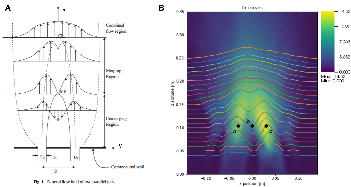
\includegraphics[width=14.7cm]{mixing_state_v4.pdf}}
    \slantedcaption{A. Definitions of three mixing states, taken from \cite{Durve2012Numericalinvestigationof}. B. TFI field on a 2D cross-section at $y$ = \SI{0.09}{\meter} and 1D profiles. Points a, b, and c are the reference points used for 1D sequential analysis.}
    \label{fig:mixing_state}
\end{figure}

\cite{Durve2012Numericalinvestigationof} also carried out a comparative study on several models for predicting the mean temperature field and temperature fluctuation field caused by mixing phenomena of the three jets \parencite{Durve2010Thermalstripingin}.
They performed a comparative study of root mean square temperature 1D profiles along the $x$ axis depending on the distance from the flow outlet,
i.e. the $z$ altitude direction in our study, Figure \ref{fig:durve2010}.
A comparison was done between one experimental ($\circ$) and three numerical simulation results (lines).
Each image in this figure shows the root mean square value of temperature measured/estimated for each normalized altitude $y/D_n$.
$y$ stands for the distance from the outlet of the jets, and $D_n$ is the diameter of the outlet.
The length along the horizontal direction ($x$ axis) is also normalized in the same way with the direction of altitude as $x/D_n$.
The root mean square values are also normalized by the temperature difference of the cold and hot jets ($\Delta T$).
The curves at each altitude do not match very well because of the difference of the compared model geometries.
For all experiment/simulation data, one can see the same transient behavior of the shape of curves, i.e.
the curves have two peaks at lower altitude, then these two peaks start to merge when the altitude increases, and finally the peaks merge completely.
Following different authors we choose to analyze the temperature in the medium using an index called the Temperature Fluctuation Intensity (TFI).
We use the definition of TFI as
\begin{align}\label{eq:4_1}
    TFI(\boldsymbol{r})=\sqrt{\frac{1}{N}\sum_{i=1}^{N}(T(i,\boldsymbol{r})-\bar{T}(\boldsymbol{r}))^2}, r=(x,y,z) \, ,
\end{align}
where
$\boldsymbol{r}$ is the spatial position vector,
$i$ is the time step number,
$N$ is the total number of time steps,
$T(i,\boldsymbol{r})$ is the temperature value at time step $i$ and position $\boldsymbol{r}$, and
$\bar{T}(\boldsymbol{r}) = \frac{1}{N}\sum_{i=1}^N T(i,\boldsymbol{r})$ is the average temperature at $\boldsymbol{r}$.
We process the PLAJEST Computational Fluid Dynamics (CFD) data to calculate the TFI index in order to compare the global behavior of the jets with these previous studies.
Figure \ref{fig:comp_durve2010} shows the same profile analysis with TFI values.
The normalized altitude $y/D_n$ and normalized horizontal position $x/D_n$ are adjusted to be the same as in \cite{Durve2012Numericalinvestigationof}'s figures.
TFI values are also normalized with $\Delta T =$ \num{43}\textdegree{}C, which is the temperature difference of the jets in the PLAJEST configuration.
Because of the difference of geometry and also of the medium (PLAJEST uses liquid sodium but the other studies use air or other liquids), the magnitude of the curves is not identical.
However, the shape of the curves follows the same way (i.e. two separated peaks $\rightarrow$ the peaks are merged gradually $\rightarrow$ the peaks are merged completely).

\begin{figure}[htbp]
    \centerline{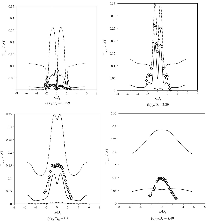
\includegraphics[width=12.0cm]{durve2010.pdf}}
    \slantedcaption{Comparison of normalized root mean square of temperature, taken from \cite{Durve2010Thermalstripingin}.}
    \label{fig:durve2010}
\end{figure}

Figure \ref{fig:mixing_state} B is the 2D cross-section at $y$ = \SI{0.09}{\meter} of the calculated 3D TFI field from the CFD results of PLAJEST.
There are three jets in the configuration of PLAJEST (the center position of the jets are $x$ = \SIlist{-0.070;0.0;0.070}{\meter}).
Between each jet, two zones with high TFI value arise by the interaction of these jet flows.
From this TFI field, it is found that for the shape of the TFI profile depending on the altitude, it seems to be possible to define three zones in a similar way as with the three zones for the mean flow field explained above.
First, the two high TFI zones arise around altitude $z$ = \SI{0.05}{\meter} and these two zones are completely separated.
Around altitude $z$ = \SI{0.09}{\meter} or lower altitude, the beginning of merging of the high TFI zones becomes clear (the lowest TFI value between two peeks starts to increase).
Here there would be some specific point that we call a merging point of the TFI zone.
The merging of these two zones is confirmed when the altitude becomes higher, and then around altitude $z$ = \SI{0.19}{\meter} these two zones are completely merged (the peak of the 1D TFI curve becomes a single one). We call this altitude a combining point of the TFI zone.

In the following section, we will carry out a more detailed analysis to verify the variations of the TFI profiles and the definition of these two points.
When we analyze the results of acoustic simulation, these two altitudes will be referred to and compared with the thermo-hydraulic state.
Thus, the main objectives of this chapter are to
see how an acoustic wave propagation fluctuation changes depending on the state of mixing flows.
In particular, we will try to find the relation between acoustic fluctuations and the changing points of the TFI 1D curves, which likely divide the TFI field into three zones (converging, merging and combined regions) as mentioned above.

\begin{figure}[htbp]
    \centerline{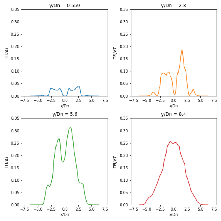
\includegraphics[width=12.0cm]{comp_durve2010.pdf}}
    \slantedcaption{Comparison of TFI 1D profiles calculated from the PLAJEST CFD results.}
    \label{fig:comp_durve2010}
\end{figure}

\section{Definition of the insonified volume}

The insonified volume is defined as a part of the PLAJEST volume displayed as a purple box in Figure \ref{fig:plajest_geo}.
In the geometry of PLAJEST, three sodium jets outflow from gaps with a \SI{20}{\milli\meter} width.
Multiple simulations are carried out with changing the $z$ coordinate of the extracted region from \SI{40}{\milli\meter} to \SI{340}{\milli\meter} above the outlet, with intervals of \SI{10}{\milli\meter}.
The temperature pattern just above the outlets is simple and stable, while it becomes more complex and unstable when the $z$ coordinate increases.
The magnitude of the fluctuations may be seen based on TFI visualization in Figure \ref{fig:mixing_state} B.
Multiple insonified volumes are then defined with the same volume size, same relative positions of the acoustic source and signal observing surfaces and with different altitudes.
In each insonified volume, a circular plane source is defined as in Figure \ref{fig:plajest_src}.
The color shows the maximum amplitudes of the emissions at each point normalized by the maximum amplitude at the center of the circle.
The plane source is composed of monopole point sources on a circular plane with a diameter of \SI{0.0254}{\meter} (i.e. 1 inch).
The intervals of each point sources are the same as the element size of the SPECFEM mesh.
Each source point emits a \SI{1}{\mega\hertz} Ricker wavelet (second derivative of a Gaussian) at the same time.
The maximum amplitude of each emission is multiplied by a Hamming window function depending on the distance from the center of the circle.
Figure \ref{fig:plajest_rec_def} shows the definitions of the observation surfaces of the acoustic signals.
On each plane, the receiving points where acoustic signals are recorded are placed with a \SI{0.0005}{\meter} pitch.
Figure \ref{fig:plajest_receiver_plane_geo} shows the positional relation between the insonified volume (central altitude $z$ = \SI{0.1}{\meter}) and the geometry of PLAJEST.
The numbers in meters show the distance from the source to each $y$-$z$ receiver plane.
The near field limit, called Io, is calculated to be \SI{67.17}{\milli\meter} using Equation \ref{eq:3_1}
and an average temperature of \num{333.167}\textdegree{}C (\num{606.317}\textdegree{}K), considering a transducer with a \num{1} inch diameter and \SI{1}{\mega\hertz} frequency.
In this virtual setup, only the first two observation surfaces are in the near field.
Thus, in the following analysis we mainly have acoustics virtual measurements in the far field.
In the PLAJEST coordinates the limit of the near field is $x$ = \SI{-0.061}{\meter}.

\begin{figure}[htbp]
    \centerline{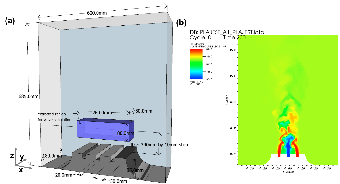
\includegraphics[width=16.0cm]{plajest_geo_v2.pdf}}
    \slantedcaption{(a) Geometry of the PLAJEST CFD simulation.  (b) Snapshot of the CFD result at time \SI{200.0}{\second}, $x$-$y$ cross-sectional plane at $y$ = \SI{0.09}{\meter}.
    Visualization for this image is done with VisIt, an open source visualization tool for massive scientific data \parencite{Childs2012VisItAnEnd}.}
    \label{fig:plajest_geo}
\end{figure}

\begin{figure}[htbp]
    \centerline{\includegraphics[width=13.0cm]{plajest_src.pdf}}
    \slantedcaption{The circular source plane used for the simulations.}
    \label{fig:plajest_src}
\end{figure}

\begin{figure}[htbp]
    \centerline{\includegraphics[width=13.0cm]{plajest_rec_def.pdf}}
    \slantedcaption{Positions of the plane source (blue) and receiver surfaces (orange and red). The $x$ position of the source plane is \SI{-0.128}{\meter}.}
    \label{fig:plajest_rec_def}
\end{figure}

\begin{figure}[htbp]
    \centerline{\includegraphics[width=18.0cm]{plajest_receiver_plane_geo_v3.pdf}}
    \slantedcaption{Relation of the positions in an insonified volume (central altitude $z$ = \SI{0.1}{\meter}) and the geometry of PLAJEST.
The points A, B and C are the positions of the reference points used for temporal analysis.}
    \label{fig:plajest_receiver_plane_geo}
\end{figure}

\section{Mesh generation and interpolation of the temperature field from Tetra4 elements to Hexa27 elements}

CEA/STMF used a numerical code for CFD calculations called TrioCFD (known as Trio\_U by 2015) for this PLAJEST numerical simulation, and LES was selected as the turbulence model.
Tetrahedral elements with 4 nodes were used for the TrioCFD calculations. The total number of elements was \num{5582706} and the characteristic mesh length was set to \SI{1.40}{\milli\meter}. We removed the first \SI{200}{\second} of their calculation from their result because that duration corresponds to the stabilization of the flow state.
Thus, \numrange{200}{210}\si{\second} with a time step of \SI{0.1}{\milli\second} is available as candidates for our wave simulation.
Three jets of sodium exist in this setup. Sodium with lower temperature (304.5\textdegree{}C) is emitted from the central jet, and with higher temperature (347.5\textdegree{}C) from the two outer jets. The average flow velocity is \SI{0.51}{\meter\per\second} for every jet (Figure \ref{fig:plajest_jaea} B).
The simulated temperature field at time = \SI{200.000}{\second} is shown in Figure \ref{fig:plajest_cea} (C). Their simulation results are in good agreement
with the experiment results obtained by JAEA in terms of normalized time-averaged temperature, normalized time-averaged temperature fluctuations, spectral power density and standard deviation of temperature values (Figure \ref{fig:plajest_cea} A, B and D).

For their calculation, a tetrahedral unstructured staggered mesh was used.
Temperature field values are defined at the center of each TrioCFD's tetrahedral mesh element, and flow velocity values are defined on the vertex nodes.
We thus had to transfer these values to our hexahedral mesh for SPECFEM3D.
To do so, we used interpolation onto each node of the SPECFEM3D hexahedral mesh using the simulation data management tool called MEDCoupling.
MEDCoupling is part of the pre-/post-processing platform SALOME (\url{http://www.salome-platform.org}) and is also available independently as a library.
Figure \ref{fig:temp_field_interpolation_processs} shows the temperature field data transfer and mesh generation steps as a pre-process for SPECFEM3D simulation.
Our hexahedral mesh for SPECFEM3D is built using the meshing software CUBIT developed by Sandia National Laboratories (USA).
Figure \ref{fig:interp_examp} shows some examples of this step. It is possible to select an arbitrary volume to be extracted from the entire geometry
and meshing is completed automatically, including the assignment of material characteristics and absorbing surface flags (the fluctuation of the temperature field may be defined later).
In this step, the region to be used for wave propagation simulation is specified in order to eliminate acoustically uninteresting parts from the PLAJEST geometry and thus reduce the required amount of computer memory, which is one of the limitations of wave simulations in large 3D models.
In order to speed-up this conversion process, we used the IOSS (IO Systems) library included in the finite-element analysis supporting software called SEACAS, also developed by Sandia National Laboratories.
After finishing preparation of mesh data, we carried out the temperature field transfer, i.e. interpolation of temperature values defined at the barycenter of each tetrahedral finite element to corner nodes of our hexahedral spectral elements.
The flow velocity data is not used for our simulation because we apply the frozen fluid hypothesis, as in \parencite{Massacret2012Simplifiedmodelingof}.
The conversion of the temperature field from TrioCFD tetrahedral mesh to SPECFEM3D nodes is done by using MEDCoupling.
Because the mesh-to-node transfer function does not support HEXA27 (second-order hexahedral finite elements), if the interpolation-target mesh is of HEXA27 type,
then HEXA27 first needs be split into eight parts of HEXA8 type (first-order hexahedral finite elements).

Determination of the element size to use in our simulations is done based on two conditions, which are the CFL condition (Equation \ref{eq:4_810}) and the number of
elements per one wave length:
\begin{align}\label{eq:4_810}
    C_p\frac{\Delta t}{\Delta x_{gll}} \leq \alpha \, ,
\end{align}
where $\Delta t$ is the time step and $\Delta x_{gll}$ is the minimum interval between two GLL grid points.
We selected the averaged Courant number $\alpha$ = \num{0.4} and the wave celerity $C_p$ = \SI{2416.268}{\meter\per\second} (in sodium with the lowest
temperature value \num{274.5} \textdegree{}C in the CFD simulation) for the calculation of the mesh size and time step duration.
In equation \ref{eq:4_810}, $\Delta x_{gll}$ is not the mesh size itself, it is the interval between GLL grid points inside the spectral elements.
This led us to use a mesh size $\Delta x$ = \SI{8.05d-4}{\meter} and a time step of \SI{2.3d-8}{\second}.
We will simulate a total of 5000 steps in order to have a sufficient total physical duration for the waves to travel through
the entire simulation domain. The mesh used in our simulations thus \num{3250000} spectral elements and a total number of GLL grid nodes of \num{215320764}.

\begin{figure}[htbp]
    \centerline{\includegraphics[width=18.0cm]{temp_field_interpolation_processs_v5.pdf}}
    \slantedcaption{Explanation of data processing for mesh generation and preparation of the heterogeneous medium to use for our acoustic calculations.}
    \label{fig:temp_field_interpolation_processs}
\end{figure}

\begin{figure}[htbp]
    \centerline{\includegraphics[width=17.0cm]{interp_examp_v2.pdf}}
    \slantedcaption{Examples of some interpolations of temperature fields from a tetrahedral mesh to a hexahedral mesh using the MEDCoupling pre/post-processing library.
The temperature field in the tetrahedral elements is indicated with transparent color on the interpolated field of the hexahedral mesh.
    The image on the left side is a close-up on one of these three examples.}
    \label{fig:interp_examp}
\end{figure}

\begin{figure}[htbp]
    \centerline{\includegraphics[width=16.0cm]{real_temp_field_sample.pdf}}
    \slantedcaption{One of the heterogeneous temperature fields used for our 3D wave propagation calculations. This field is taken from time step number 10,
and the central altitude of the calculation domain is \SI{0.1}{\meter} from the sodium outlet.
    One mesh contains 3,250,000 spectral elements and the total number of Gauss-Lobatto-Legendre grid points is 215,320,764.}
    \label{fig:real_temp_field_sample}
\end{figure}


\section{Results of acoustic wave propagation in a single temperature field}

In this part, we analyze the sensitivity of ultrasound to thermo-hydraulic changes.
The goal is to study how the ultrasonic beam is deflected or deformed by the temperature field.
In the following section, we will study the evolution of measurements as a function of time.

\begin{figure}[htbp]
    \centerline{\includegraphics[width=16.0cm]{3dwavefronts_v3.pdf}}
    \slantedcaption{Visualization of the 3D wave front using contouring and clipping, at position $x$ = A) \SI{0.105}{\meter} and B) \SI{-0.035}{\meter} calculated at altitude $z$ = \SI{0.14}{\meter}, time = \SI{200.010}{\second} of PLAJEST with a heterogeneous medium temperature.}
    \label{fig:3dwavefronts}
\end{figure}

Figure \ref{fig:3dwavefronts} shows the visualized 3D wave fronts based on 3D contour visualization.
These waves are visualized from signals received in the $y$-$z$ receiver planes at time = \SI{200.010}{\second} in the CFD simulation and at altitude $z$ = \SI{0.14}{\meter}.
The left image is the wave front recorded at $x$ = \SI{0.105}{\meter} and the right image is recorded at $x$ = \SI{-0.035}{\meter}.
Color variations represent the signal amplitude values.
Blue is negative and red is positive.
In order to show the inside structure of the wave front, some contour surfaces are clipped off of its half or quarter volume.
The red part has higher pressure values and the blue part has lower ones.
The $y$ and $z$ axes correspond to the $y$ and $z$ axes of the PLAJEST geometry.
The $x$ axis indicates time.
For this 3D visualization, we used a VTK file (Visualization Toolkit: an open-source, freely available software system for 3D computer graphics, image processing, and visualization. \url{http://www.vtk.org}) that we displayed with the visualization software VisIt.
The visual information reveals that the wave fronts having passed through heterogeneous liquid sodium are deflected and deformed but that the amount of wave deformation is not so large.
The wave forms are different between waves passing from the end of the near field region to a far longer distance in the far field region (almost 4 $\times$ Io, where Io is the near field limit), and the wave front in the near field has the shape that is more complex than in the far field, as expected.
We will carry out a quantitative analysis of the amount of modification in the latter part of this chapter.
Figure \ref{fig:plajest_res1} shows part of the acoustic fields obtained from all of the simulations. Here an acoustic field refers to the maximum pressure values at each spatial point.
In figure \ref{fig:plajest_res1}, acoustic fields in the $x$-$y$, $y$-$z$ and $y$-$z$ plane (for $x$ = \SIlist{0.035; 0.105}{\meter}) are indicated for the simulations whose middle $z$ coordinate value are $z$ = \SIlist{0.04; 0.12; 0.24; 0.34}{\meter}. Additionally, the top row shows the results for the case with a homogeneous medium. In the homogeneous case, the temperature of medium was set to 333.167\textdegree{}C, which is the ambient temperature value of the CFD calculations.
From this figure, we find that the acoustic field at $z$ = \SI{0.040}{\meter}, which is close to the outlets, and the homogeneous case are quite similar.
This comes from the fact that the temperature boundary just above the outlets is almost orthogonal to the direction of wave propagation.
Also at z = \SI{0.340}{\meter}, the mixing of the hot and cold jets has matured enough and the magnitude of the temperature difference becomes small;
therefore, a wave is less affected by the heterogeneity at this altitude. However, at $z$ = \SIlist{0.120; 0.240}{\meter}, it can be seen that the acoustic fields
are bent by the heterogeneity of the field, and the reduction of maximum amplitude values with increasing propagation distance becomes greater.
This first qualitative description is then shown in Figure \ref{fig:plajest_res2} with 1D profiles of the acoustic field.

In Figure \ref{fig:plajest_res2}, values of the acoustic fields on the $z$ axis of each $y$-$z$ receiver planes are indicated.
The red lines represent the results of the homogeneous case and the blue lines represent all the results for the heterogeneous cases at each $z$ position of the simulation domain.
Amplitude values are normalized by the maximum amplitude (i.e. pressure) for all simulations.
How the maximum amplitude of pressure recorded in each $y$-$z$ receiver plane changes depending on the positional changes in the $z$ direction of the simulation domains is indicated in Figure \ref{fig:plajest_res3}.
At planes $x$ = \SIlist{-0.105; -0.080}{\meter}, i.e. near the plane source, maximum amplitudes take approximately constant values regardless of distance from the outlets.
In contrast, at the farthest and second farthest $y$-$z$ planes at $x$ = \SIlist{0.105; 0.080}{\meter}, it is found that the amplitude value of the simulation domain $z$ = \SI{0.120}{\meter} is approximately 10 \% smaller than the other values. At the same time the second peak may be found at $z$ = \SI{0.240}{\meter}.
It is considered that the effect of temperature heterogeneity becomes stronger under two conditions, which are:
\begin{itemize}
\item mixing of hot and cold flow are developed enough so that the shape of the temperature boundary is curved and not parallel to the emitted wave front,
\item the temperature difference remains large.
\end{itemize}
The altitude $z$ = \SI{0.120}{\meter} is the distance from the outlets where the temperature boundary starts to be changed while the temperature difference is still relatively still compared to the region above.
On the other hand, it seems that, at $z$ = \SI{0.240}{\meter}, the temperature difference is already small and even smaller than at $z$ = \SI{0.230}{\meter}.
This might be caused by the fact that the temperature boundary shape became a key factor for the whole effects rather than the temperature difference only.
As a result, we find that there is a certain relationship between the strength of effects of temperature heterogeneity on acoustic fields and the distance from the outlets of the sodium jets, i.e. the state of mixing flows. More precisely, the importance of these effects on maximum acoustic pressure can vary up to about 10 \% at a certain altitude.
Accordingly, we may assume that the magnitude of the temperature difference in a medium and the shape of the temperature boundary are the key factors
that govern the cumulated effects of medium heterogeneity on wave propagation.

A single time step was examined for this first study. In the next \autoref{sec:res_multi_time}, we will perform simulations with the same PLAJEST configuration for other time steps extracted from the CFD calculation in order to search for a relation between the strength of the medium heterogeneity and the variations of the ultrasonic signals.

\begin{figure}[htbp]
    \centerline{\includegraphics[width=16.0cm]{plajest_res1_v2.pdf}}
    \slantedcaption{Acoustic fields obtained from all the simulations.}
    \label{fig:plajest_res1}
\end{figure}

\begin{figure}[htbp]
    \centerline{\includegraphics[width=12.0cm]{plajest_res2_v2.pdf}}
    \slantedcaption{Values of the acoustic fields on the $z$ axis at $y$ = 0 of each $y$-$z$ receiver plane.}
    \label{fig:plajest_res2}
\end{figure}

\begin{figure}[htbp]
    \centerline{\includegraphics[width=14.0cm]{plajest_res3_v2.pdf}}
    \slantedcaption{The maximum amplitude of pressure recorded in each $y$-$z$ receiver plane changes depending on the positional change in the $z$ direction of the simulation domain.}
    \label{fig:plajest_res3}
\end{figure}

\section{Analysis of time-varying temperature fields of PLAJEST} \label{sec:res_multi_time}

\subsection{Selection of the CFD time steps to extract and analyze}

    The CFD calculation carried out by CEA STMF has approximately \SI{10}{\second} in total, from \SI{200.000}{\second} to \SI{210.197} with a \SI{0.001}{\second} interval.
The initial \SI{200}{\second} of the calculation was dedicated to ensuring stabilization of the flow and are thus excluded in our analysis.
    Because of the limitation of allocated computation time on the supercomputer that we use for this thesis, it was not possible to run the temperature field interpolation and wave propagation calculation processes for all of these CFD time steps.
    Instead, we had to extract several time steps of the temperature field with a wider interval from the CFD results.
    In order to select the time step interval to extract for our acoustic simulation, we used the power spectrum density curve \parencite{Angeli2015LargeEddySimulation} (Figure \ref{fig:PSD_angeli}, blue line). This curve indicates the temperature history at $x$ = \SI{-0.015}{\meter} (between the left and center jets), $y$ = \SI{0.09}{\meter} (middle point on the $y$ axis) and $z$ = \SI{0.1}{\meter}.
    From this curve, its peak is found lower than \SI{5}{\hertz} (around \SI{3}{\hertz}).
    Thus, to be sure to include the frequency of this \SI{5}{\hertz} temperature fluctuation, we extracted the temperature fields with a \SI{0.1}{\second} interval (i.e. \SI{10}{\hertz}).
    In a first approximation the peak was estimated to be around \SI{2}{\hertz}, and in that case we could expect to have 5 points per period to keep the peak at \SI{2}{\hertz}.
    This is the limit of Shannon's sampling criterion.

\begin{figure}[htbp]
    \centerline{\includegraphics[width=12.0cm]{PSD_angeli.pdf}}
\vspace*{-1.6truecm}
    \slantedcaption{Normalized PSD curves of temperature history in the CFD calculation (blue line) at $x$ = \SI{-0.015}{\meter}, $y$ = \SI{0.09}{\meter} and $z$ = \SI{0.1}{\meter}, taken from \cite{Angeli2015LargeEddySimulation}. Normalized PSD curves are calculated by dividing the original PSD with the maximum PSD value.}
    \label{fig:PSD_angeli}
\end{figure}

    Figure \ref{fig:timestep_extraction} shows this relation between the CFD time steps and the extracted (sub-sampled) time steps for our acoustic simulations.
    Figure \ref{fig:psd_finer} shows the temperature histories and PSD curves of the original CFD results at three selected points, and Figure \ref{fig:psd_coarser} shows the same kind of curves but with only extracted time steps.
    These three points have the same $y$, $z$ position ($y$ = \SI{0.09}{\meter} and $z$ = \SI{0.1}{\meter}) and a different $x$ position ($x$ = \SIlist{-0.035;0.0;0.035}{\meter}).
    $x$ = \SIlist{-0.035;0.035}{\meter} are the positions between the two jets, and thus where the TFI will be higher than in the other areas.
    $x$ = \SI{0.0}{\meter} is in the middle of the central jet.
    These three points were selected in order to examine the thermo-hydraulics regime in three characteristic areas.
    The positional relation with the PLAJEST geometry is indicated by points A,B,C in Figure \ref{fig:plajest_receiver_plane_geo},
and the relation with the TFI is indicated by points a,b,c in Figure \ref{fig:mixing_state}.
    Using all the time steps of the CFD results, we calculated the PSD curves (Figure \ref{fig:psd_finer}).
    The peak of the PSD curve is confirmed at \SI{3}{\hertz}.
    Then PSD curves calculated from the coarser time step that we use in our acoustic simulations shows that the peak frequency at \SI{3}{\hertz} is conserved for the central point.
    From this comparison, we thus verify that the peak frequency of the temporal temperature fluctuation remains lower than the frequency limit that we selected for our acoustic simulation.
    Let us note however than in future work we plan to perform new calculations with a refined time step to describe these peaks more finely.

\begin{figure}[htbp]
    \centerline{\includegraphics[width=11.0cm]{timestep_extraction.pdf}}
    \slantedcaption{Sampling intervals for the original CFD simulation and for our wave propagation simulation.}
    \label{fig:timestep_extraction}
\end{figure}

\begin{figure}[htbp]
    \centerline{\includegraphics[width=20.0cm]{psd_finer_v2.pdf}}
    \slantedcaption{A. PSD curves and B. temperature histories of the CFD results at three different $x$ positions ($y$ = \SI{0.09}{\meter}; $z$ = \SI{0.1}{\meter}), with a 10 Hz sampling.}
    \label{fig:psd_finer}
\end{figure}

\begin{figure}[htbp]
    \centerline{\includegraphics[width=20.0cm]{psd_coarser_v2.pdf}}
    \slantedcaption{A. PSD curves and B. temperature histories of the extracted time steps at three different $x$ positions, with a 10 Hz sampling.}
    \label{fig:psd_coarser}
\end{figure}

\subsection{Treatment of the massive amount of calculations and management of the results}

    In this study, all of simulations were performed on two of the largest supercomputers in Europe: CURIE (CEA TGCC) and OCCIGEN (CINES), both part of GENCI (Grand \'Equipement National de Calcul Intensif).
    The computation domain was divided into 256 parts, and parallelized calculations were carried out.
    The average duration for an acoustic simulation is about 26 minutes, excluding mesh generation and the interpolation processes of the temperature fields, which are done once and for all.
    The duration of the interpolation of a temperature field from a TrioCFD result to SPECFEM3D is approximately 20 hours using a single CPU for one acoustic simulation altitude of one time step.
    We carried out 70 time steps of interpolation of the 3D temperature field, for 22 difference altitudes, resulting in a total of 1540 acoustic simulations to perform.
As a result, the total time needed for a complete simulation of wave propagation over \SI{7}{\second} of the variable thermo-hydraulic regime is approximately equal to 687 hours, i.e. 29 days.
    Because of the huge number of calculations, the result data cannot be conserved as a 3D volume data because of the limitation of allocated storage on supercomputers.
    Instead of storing all results in 3D, we first selected the 2D planes in which we will analyze the acoustic signals (Figure \ref{fig:plajest_rec_def}).
    We then defined time windows for each $y$-$z$ plane to cut the received signals depending on the arrival time of the wave front.
    These time-windowed signals were then gathered as a single, huge HDF5 binary file.
    The HDF5 (Hierarchical Data Format) format is a standard and widely-sued binary file format that has been developed to manage extremely large and complex data collections.
    By using it, one can access the results faster than with other standard file formats such as e.g. ASCII, json, csv, pickle (Python-friendly binary data format) etc.

\subsection{Computing TFI data for comparison with acoustic simulation results}

    As introduced in Equation \ref{eq:4_1}, we resort to an index called Temperature Fluctuation Intensity (TFI), as used in \cite{Angeli2015LargeEddySimulation}.
    Because of the very large numbers of total time steps and also the huge number of mesh nodes included in the CFD calculation results,
the standard way to calculate the TFI value based on this equation is not very efficient.
    To calculate that TFI, we thus selected and implemented another, more advanced algorithm: the online algorithm, which we will briefly describe in this section.
    Figure \ref{fig:tfi3d} shows the calculated TFI field in 3D, and Figure {\ref{fig:tfi_with_field}} is the cross-section at $y$ = \SI{0.09}{\meter}.
We find that there are two areas where the TFI value becomes high between the sodium jets at altitude $z$ = \SIrange{0.08}{0.16}{\meter}.
    It should also be noted that the TFI field is not symmetric with respect to the $x$ center.

    The online algorithm calculates some field value from serial data sequentially and based on a single step \parencite{Knuth1997TheArtof}.
    This algorithm can be required for serial data for which each step needs a large amount of computer memory and/or when the number of serial data
is so large that it is very expensive to perform an entire loop of calculations more than twice.
    We thus applied this algorithm to compute the TFI, i.e. the standard deviation of the temperature value at a given point,
    because computing a standard deviation implies several loop over the whole time steps, first to calculate the mean temperature,
and second to calculate the difference between a temporal value and the mean value.
    The PLAJEST CFD data comprise 10,000 time steps of 3D volume data with 2,039,769 mesh elements.
    One entire loop calculation for this data takes about 10 hours.
    By applying the online algorithm for the calculation of the TFI, we only need to do this long loop calculation once.

\begin{figure}[htbp]
    \centerline{\includegraphics[width=10.0cm]{tfi3d_v3.pdf}}
    \slantedcaption{Visualized 3D TFI field.}
    \label{fig:tfi3d}
\end{figure}

    \begin{figure}[htbp]
        \centerline{\includegraphics[width=12.0cm]{tfi_1d_v2.pdf}}
        \slantedcaption{TFI values on the $x$ axis and at $y$ = \SI{0.09}{\meter} at several altitudes.}
        \label{fig:tfi_1d}
    \end{figure}

    The definition of standard deviation of temperature at a given position $\boldsymbol{r}$ is
    \begin{align}\label{eq:4_2}
        \sigma^2 (\boldsymbol{r}) = \frac{1}{N}\sum_{i=1}^{N} (T(\boldsymbol{r},i) - \bar{T}(\boldsymbol{r}))^2 \, ,
    \end{align}
    where $N$ is the total number of time steps and $\bar{T}(\boldsymbol{r})=\frac{1}{N}\sum_{i=1}^{N}T(\boldsymbol{r},i)$ is the average temperature at position $\boldsymbol{r}$.
    In the online algorithm, the averaged value $\bar{T}(\boldsymbol{r},n)$ and the term $\sum_{i=1}^{n} (T(\boldsymbol{r},i) - \bar{T}(\boldsymbol{r}))^2 = M_{\boldsymbol{r},n}$
    are sequentially updated for each time step during the entire loop calculation.
    For each time step at $n$,
    \begin{align}\label{eq:4_3}
        \bar{T}_{\boldsymbol{r},n} = \bar{T}_{\boldsymbol{r},n-1} + \frac{T_{\boldsymbol{r},n} - \bar{T}_{\boldsymbol{r},n-1}}{n}
    \end{align}
    \begin{align}\label{eq:4_4}
       M_{\boldsymbol{r},n}=M_{\boldsymbol{r},n-1}+ (T_{\boldsymbol{r},n} - \bar{T}_{\boldsymbol{r},n-1})(T_{\boldsymbol{r},n} - \bar{T}_{\boldsymbol{r},n})
    \end{align}
    The standard deviation calculation is then finalized as
    \begin{align}\label{eq:4_5}
        \sigma_{\boldsymbol{r}}=\sqrt{\frac{M_{\boldsymbol{r},N}}{N}} \,.
    \end{align}

   \begin{figure}[htbp]
        \centerline{\includegraphics[width=12.0cm]{tfi_with_field.pdf}}
        \slantedcaption{TFI curves corresponding to the 2D TFI field. The left side shows the $z$ altitude where those lines are extracted.}
        \label{fig:tfi_with_field}
    \end{figure}

    Figure \ref{fig:tfi_1d} shows the TFI values on the $x$ axis of $y$ = \SI{0.09}{\meter} at several altitudes (i.e. $z$ positions), and Figure \ref{fig:mixing_state} B represents these TFI curves drawn in the case of the 2D TFI field.
    The maximum TFI value is found at around altitude $z$ = \SI{0.13}{\meter}. The change of shape of the curves depending on the distance from the exit of the jets seems to match with the result of \cite{Durve2010Thermalstripingin},
    i.e. the curves at low altitude have two TFI peaks, and then these peaks gradually merge when the $z$ altitude increases.
    We will further analyze this effect in the next sections of this chapter.

\subsection{Calculating the "Cumulated TFI" (CTFI) value}

    The TFI calculated above is the index that evaluates the intensity of the fluctuation at one spatial point,
while acoustic wave propagation will be affected not only by one position but by the whole state along its propagation path.
    Thus, in order to find the appropriate thermo-hydraulic index for comparison in the case of a propagating wave, we define a new index, which we call the cumulated TFI (CTFI).
    The CTFI is the value that indicates the amount of TFI that the acoustic wave experiences along the central axis.
    We define the CTFI at the position $x_p$ in the propagation direction by
    \begin{align}\label{eq:4_6}
        {I_c}(x_p,z_{alt},R) = \int_{x_{s}}^{x_{p}} \int_0^R \int_0^{2\pi} I(r,\theta,z_{alt}) w(r) d\theta dr dx \,
    \end{align}
    where
    $I_c$ is the CTFI value,
    $I(x,r,\theta)$ is the TFI value at $x,r,\theta$,
    $x_s$ is the x coordinate of acoustic source,
    $z_{alt}$ is the altitude (along the $z$ axis) of the center of the acoustic source plane,
    $R$ is the distance from the central axis, and
    $w(r)$ is a weight function to make TFI values near the central axis have more effect and TFIs far from the central axis less effect.
One can define several versions of the CTFI, for instance:
\begin{enumerate}
\item CTFI in 1D (integrated on the central $x$ axis), with $w(r) = 1$ and $R = $ one mesh element size,
\item CTFI in 3D A (integrated in a domain where the acoustic beam passes), with $w(r) = 1$ and $R = $ the radius of the acoustic source, i.e. 1.27 cm,
\item CTFI in 3D B (integrated in a cylindrical volume where the acoustic beam passes, with a weighting function $w(r) = 0.54 + 0.46 cos{\pi \frac{r}{R}}$ and $R = $ the radius of the acoustic source, i.e. 1.27 cm.
\end{enumerate}
Using a larger $w(r)$ allows us to take into account the whole ultrasonic beam.
A more complex function will be needed to take into account the beam divergence.
In this thesis, we only use the first definition of the CTFI, i.e. the CTFI in 1D, as a first analysis.
The other possible choices may be examined in future work.

Figure \ref{fig:ctfi_1d} indicates the CTFI curves on the $x$ axis at $y$ = \SI{0.09}{\meter} and at several $z$ altitudes.
The left image shows the CTFI depending on the $x$ position, i.e. the propagation distance. The source plane is positioned at $x$ = \SI{-0.128}{\meter}.
Each line represents the $z$ altitude at which the curves are extracted.
The magnitude of the CTFI becomes largest around the altitude $z$ = \SI{0.13}{\meter}.
The curves for a lower $z$ altitude exhibit a two-step increment, as there are two peaks of TFI as we saw in the last section.
At a position higher than \SI{0.16}{\meter}, this two-step increment is no longer seen.
The right image represents the CTFI values versus altitude $z$.
Each line represents the $x$ position, i.e. propagation distance (the acoustic source is placed at $x$ = \SI{-0.128}{\meter}).
The farther the $x$ position becomes, the larger the magnitude of the CTFI becomes as well.
We find that the peak of the CTFI positions is around \SIrange{0.13}{0.15}{\meter}.
For the $x$ position = \SI{0.00}{\meter} just after the first (left side of) the high TFI zone and the middle of the central jet,
the CTFI peak is slightly shifted to a higher $z$ altitude.
This is caused by the slight difference is the shape and position of the high TFI zones, as one can see in Figure \ref{fig:ctfi_with_field}.
Figure \ref{fig:ctfi_2nd} shows the second derivatives of the CTFI curves.
The inflection points are found around $z$ = \SI{0.09}{\meter} and \SI{0.19}{\meter}.
These points are the same altitudes as what we defined as the merging point and combining point of the standard TFI.
Thus, from this result, we find that we can define the merging and combing points of the TFI as the inflection points of the second derivatives of the CTFI curve.

In the following part of this chapter, we will study the acoustic fluctuation state based on these merging and combining points.

\begin{figure}[htbp]
    \centerline{\includegraphics[width=17.5cm]{ctfi_1d_v4.pdf}}
    \slantedcaption{CTFI curves on the $x$ axis at $y$ = \SI{0.09}{\meter} and at several $z$ altitudes.}
    \label{fig:ctfi_1d}
\end{figure}

\begin{figure}[htbp]
    \centerline{\includegraphics[width=12.0cm]{ctfi_with_field.pdf}}
    \slantedcaption{CTFI curves corresponding to the 2D TFI field.
On the left side once can see the altitude $z$ at which these lines are extracted.}
    \label{fig:ctfi_with_field}
\end{figure}

\begin{figure}[htbp]
    \centerline{\includegraphics[width=12.0cm]{cfti_2nd_v2.pdf}}
    \slantedcaption{Second derivatives of the CTFI 1D profiles. Each line indicates the $x$ position.}
    \label{fig:ctfi_2nd}
\end{figure}

\section{Comparison with acoustic simulation results}

\subsection{Fluctuation of acoustic signals}

    First, we investigate the transition of the deviated wave front at the farthest $y$-$z$ receiving plane (i.e. $x$ = \SI{0.105}{\meter} and at a distance from the source of \SI{0.233}{\meter}).
    Figure \ref{fig:move_impact_points} shows the impact points, i.e. the position where the pressure value becomes maximum in the $y$-$z$ receiving plane.
In order to show temporal changes of the positions of the impact points more clearly, the positions of the impact points are linked by arrows in temporal order,
and digits are added to indicate the order in which the position of the impact point changes.
    Histograms for the $y$ and $z$ axis directions are also placed, showing the mean and standard deviation values.
    We confirm that the standard deviation is the largest at altitude $z$ = \SI{0.13}{\meter} (number 3 of \ref{fig:move_impact_points}).
    This is in good agreement with the peak $z$ position of the CTFI in Figure \ref{fig:ctfi_1d}.
    At lower altitude $z$ = \SIlist{0.04;0.09}{\meter}, the distribution of the impact points exhibits directivity, i.e. the standard deviation for the $y$-axis direction is larger than for the $z$-axis direction.
    This result illustrates the fact that the 3D temperature fluctuation pattern before maturing of the mixing state has directivity.
Namely, approximating the fluctuation of the acoustic celerity field using an isotropic Gaussian random process may not be very accurate for the regions where the flow is still strong.
    From this result, we can confirm the observation by \cite{Iooss2002Numericalsimulationof} of the non-applicability of an isotropic Gaussian random field for this region in a quantitative way.
Part of this directivity effect may be caused by the geometry of PLAJEST, because the cross-sections on the $y$ axis of PLAJEST always have the same shapes.
    However, in the real geometry of a SFR, for instance ASTRID, which has outlet tubes with a larger diameter (\SI{0.15}{\meter}) than in the PLAJEST experiment (\SI{0.02}{\meter}), the same effect may occur depending on the directions of the acoustic beam towards the sodium jets, even if the shape of the jets is cylindrical.

\begin{figure}[htbp]
    \centerline{\includegraphics[width=16.0cm]{move_impact_points_v2.pdf}}
    \slantedcaption{Movement of acoustic impact points (i.e. the position at which acoustic pressure becomes the largest) in the $y$-$z$ receiving plane at $x$ = \SI{0.105}{\meter}, and histograms for the $y$ and $z$ directions. Movements of only the seven initial time steps are indicated with red arrows and with digits in magenta.}
    \label{fig:move_impact_points}
\end{figure}

    We also carried on an acoustic fluctuation analysis.
    Figure \ref{fig:acoust_sig_1d_fluc} shows the history of maximum amplitude and the time at which the maximum amplitude is received, as well as the normalized PSD curves.
    Maximum amplitude values are taken from the envelope of each received signal.
    The figures on the left column are the history of maximum amplitude value (in blue), receiving times (in red) and temperature (in green).
    The figures on the right column are the PSD curves of the three values, in the same colors as the history curves.
    The results received at four different altitudes, at $x$ = \SI{0.105}{\meter}, $y$ = \SI{0.09}{\meter} and $z$ = \SIlist{0.04;0.09;0.14;0.21}{\meter} are shown.
    At the lowest altitude ($z$ = \SI{0.04}{\meter}), the magnitude of fluctuation of the signal is the smallest among the four positions.
    At altitude $z$ = \SIlist{0.09;0.14}{\meter}, the magnitude of fluctuation becomes larger, and then
    at a higher altitude ($z$ = \SI{0.21}{\meter}), the magnitude of fluctuation again becomes smaller than at $z$ = \SI{0.09}{\meter} and \SI{0.14}{\meter}.
    Compared with the CFTI values, the shape of fluctuation magnitude seems to match with the CTFI curve.
    From the PSD at altitude $z$ = \SI{0.04}{\meter}, the peak of both amplitude and receiving time is before \SI{1}{\hertz}.
    When the altitude becomes higher, only the peak of receiving time becomes \SI{3}{\hertz}, as the peak frequency of temperature fluctuation in Figure \ref{fig:psd_finer}.
    However, in the PSD curve of maximum amplitude, the peak seems to be found around \SI{1.8}{\hertz}, but it is weak (i.e. there are other small peaks).
    At this $x$ position, temperature fluctuation is almost zero.
    Thus it is not possible to compare the temperature fluctuation and the fluctuation of acoustic signals.
    In order to see if the fluctuation state of temperature has an effect on the acoustic fluctuation at $x$ = \SI{0.105}{\meter},
    the same history curves and PSD are indicated for different $x$ positions in Figure \ref{fig:ac_1d_comp_x}.
    At $x$ = \SI{0.0}{\meter}, maximum amplitude, receiving time and temperature have no peaks on their PSD curves.
    At $x$ = \SI{0.035}{\meter}, a peak at \SI{3}{\hertz} is found for the PSD of temperature as well as for the PSD of receiving time, but maximum amplitude has no peak.
    It should be noted that the magnitude of the temperature fluctuation is the largest among other $x$ positions.
    At $x$ = \SI{0.105}{\meter}, temperature has no fluctuation while the peak at \SI{3}{\hertz} of the PSD of receiving time remains.
    Maximum amplitude still has only a weak peak around \SI{1.8}{\hertz}.
    These results show that the fluctuation of time of flight at one receiving position may result not only from the fluctuation state of temperature at the receiving point only,
    but also from other locations around the propagation path, where the magnitude of temperature fluctuation is strong
and that may thus have a dominant effect on the acoustic signal observed later in the propagation.
    In summary, the spectral analysis of the amplitude fluctuations does not make it possible to highlight a dominant frequency. The spectrum in particular is strongly noisy.
    On the other hand, the spectrum of time of flight fluctuations, especially when they are of great amplitude (in the merging region),
reveals a dominant frequency that is consistent with the frequency of temperature fluctuations in the mixing zone.
    These preliminary results could be refined by a frequency analysis performed with a smaller time step.

\begin{figure}[htbp]
    \centerline{\includegraphics[width=17.0cm]{acoust_sic_1d_fluc_v2.pdf}}
    \slantedcaption{History of maximum amplitude (in blue), arrival time (in red) and temperature (in green), and the normalized PSD curves,
    for four different altitudes, at $x$ = \SI{0.105}{\meter}, $y$ = \SI{0.09}{\meter} and $z$ = \SIlist{0.04;0.09;0.14;0.21}{\meter}.}
    \label{fig:acoust_sig_1d_fluc}
\end{figure}

\begin{figure}[htbp]
    \centerline{\includegraphics[width=17.0cm]{ac_1d_comp_x.pdf}}
    \slantedcaption{History of maximum amplitude (in blue), arrival time (in red) and temperature (in green), and the normalized PSD curves,
    for three different $x$ position, at $x$ = \SIlist{0.0;0.035;0.105}{\meter}, $y$ = \SI{0.09}{\meter} and $z$ = \SI{0.09}{\meter}.}
    \label{fig:ac_1d_comp_x}
\end{figure}

\subsection{Standard deviation analysis}

    In order to get additional information that will help to interpret the fluctuation of the acoustic signals,
    we also carried out a standard deviation and mean value analysis for the whole of $z$ altitudes based on the following four acoustic quantities:
    \begin{itemize}
        \item maximum amplitude at the impact point and at the center of the $y$-$z$ plane,
        \item amount of deviation $r$,
        \item angle at the impact point $\theta$,
        \item receiving time of the maximum amplitude at the center of the $y$-$z$ plane.
    \end{itemize}
    Figure \ref{fig:impactpoint} shows the definition of the impact point, of $r$, and of $\theta$.

    \begin{figure}[htbp]
        \centerline{\includegraphics[width=9.0cm]{impactpoint_v4.pdf}}
        \slantedcaption{Definition of the impact point, of the amount of deviation $r$, and of the deviation angle $\theta$.}
        \label{fig:impactpoint}
    \end{figure}

    Figure \ref{fig:std_amps} shows the standard deviation and mean values of maximum amplitude values recorded at the center and at the impact point of each $y$-$z$ plane.
    Part 1 shows the standard deviation and mean value of maximum amplitudes at the center of the $y$-$z$ planes for each $z$ altitude.
    Part 2 shows the same values but recorded at the impact points.
    Each line is the mean value, and the error bar is the standard deviation at each position.
    The scale of values on the vertical axis is the same for the mean values, and the length of the error bars as well.
    We note that the mean values of maximum amplitude of each $x$ position are not very different between the different $z$ altitudes.
    In Part 3, only the mean values of maximum amplitude are plotted (solid line: $y$-$z$ center, dashed line: impact point).
At the $x$ positions far from the acoustic source ($x$ = \SIlist{0.035;0.08;0.105}{\meter}), differences of means between the $y$-$z$ center and the impact point are observed.
    This comes from the fact that the impact points always records the maximum amplitude of an acoustic wave front, thus the mean value may be larger than at the $y$-$z$ center.
    $x$ = \SI{-0.08}{\meter} is in the near-field (or Fresnel) zone, thus the difference between the maximum pressure value and the value of pressure on the axis (i.e. pressure at the center of the $y$-$z$ plane) is large.
    Part 4 shows standard deviations divided by mean values at each $z$ altitude.
    At altitudes in the range $z$ = \SIrange{0.10}{0.15}{\meter}, the standard deviation at each $x$ position becomes larger than at other altitudes.
    By applying a moving average triangular window with a window length of 8, we obtain Part 5.
    The scatter plots are the standard/mean values before smoothing, and the lines represent smoothed curves.
    The curves have similar peak positions as the CTFI curves of Figure \ref{fig:ctfi_1d} and also exhibit the same position of their inflection points when computing
their second derivatives (Part 6).
    Thus, the inflection points of standard/mean curves of maximum amplitudes occur at the altitudes of the merging point and combining point of the TFI values.

\begin{figure}[htbp]
    \centerline{\includegraphics[width=17.0cm]{std_amps_v3.pdf}}
    \slantedcaption{
    1: Comparison of maximum magnitude at the center of each $y$-$z$ receiving plane.
    2: Comparison of maximum magnitude at the acoustic impact point, i.e. the location where the pressure value becomes maximum in each $y$-$z$ plane.
    3: Comparison of the mean value of maximum amplitudes. The solid lines are the values at the $y$-$z$ plane center, and the dashed lines are the values at the impact points.
    4: Comparison of standard deviation values divided by the mean value for each $z$ altitude.
    5: Standard/mean curves smoothed by a moving average window.
    6: Second derivatives of smoothed standard/mean curves.}
    \label{fig:std_amps}
\end{figure}

    Figure \ref{fig:std_r} is the analysis of the deviation length $r$.
    Part 1 indicates mean curves with solid lines and Part 2 shows standard deviation curves.
    The peak positions are also similar with the maximum amplitude curves, i.e. the peaks of the $x$ = \SIlist{0.035;0.08;0.105}{\meter} curves occur around altitude $z$ = \SIrange{0.13}{0.14}{\meter}.
    The curves in Part 3 are smoothed mean curves, and Part 4 shows the second derivatives of these means.
    Part 5 and Part 6 are smoothed standard deviations and their derivatives.
    Using Part 4 and Part 6, we can also find the inflection points for the mean and standard deviation curves at the merging point and combining point of the TFI.

\begin{figure}[htbp]
    \centerline{\includegraphics[width=18.0cm]{std_r_v3.pdf}}
    \slantedcaption{
    1: Comparison of the mean and standard deviation of deviation length $r$. The solid line is the mean value and the dashed line is the mean plus the standard deviation.
    2: Comparison of standard deviation only.
    3: Mean curves smoothed with a moving average window.
    4: Second derivatives of the smoothed mean lines.
    5: Standard deviation curves smoothed with a moving average window.
    6: Second derivatives of the smoothed standard deviation lines.}
    \label{fig:std_r}
\end{figure}

    Figure \ref{fig:std_theta} shows the mean and standard deviations of $theta$ as defined in Figure \ref{fig:impactpoint}.
    The solid lines are the mean angles and the dashed lines are the mean plus standard deviations and mean minus standard deviations.
    At altitudes lower than \SI{0.15}{\meter}, the mean angle is shifted in the first quadrant.
    Thus, in this region, the deflection of acoustic beams has directivity.
    At altitudes higher than \SI{0.15}{\meter}, the mean angle is still shifted but from the deviation length $r$, which has smaller values at these high altitudes as seen in Figure \ref{fig:std_r}, and there is no more directivity of deflection.
    From these results, we find that the directivity of the deflection effect on acoustic propagation exists at lower altitude, where the sodium flow is still strong and mixing between jets has not matured yet.
    Because of this, the isotropic Gaussian random field representation is not applicable for this area because isotropic Gaussian fields have no directivity effects on wave propagation.
    This altitude \SI{0.15} was the position at which CTFI curves for $x$ = \SI{0.105}{\meter} became maximum.

\begin{figure}[htbp]
    \centerline{\includegraphics[width=13.0cm]{std_theta_v2.pdf}}
    \slantedcaption{Comparison of standard deviation and mean values of deviation angle $\theta$.}
    \label{fig:std_theta}
\end{figure}

    Finally, let us analyze the simulation results based on the fluctuation of times of flight, i.e. the receiving time of the signal.
    Figure \ref{fig:def_tof} shows the definition of the initial wave and of the time of flight.
    The position where simulation time is taken equal to zero is the center of the Ricker wavelet (second derivative of a Gaussian).
    We define the receiving time (the time of flight) as the peak position of the signal envelope.
    Let us recall that there are several classical (and different) ways to measure time of flight in practice.
Using the signal envelope is one of them, and it is useful in particular when the beginning of the signal can be masked by the noise \parencite{Chaki2007CombinationofLongitudinal}.
    The figures in \ref{fig:std_tof} show the change of mean and standard deviation of times of flight at each $z$ altitude of each $x$ position.
In the figure for $x$ = \SI{-0.105}{\meter}, almost no fluctuation of time of flight is found, except at altitudes in the range \SIrange{0.18}{0.22}{\meter}.
    As one can see in the TFI field of Figure \ref{fig:tfi_with_field}, even if the $x$ position is before the first jet,
a fluctuation of the medium still occurs because the fluctuating field diffuses when the flows go higher.
    At $x$ = \SI{-0.08}{\meter}, this character of the mixing jet can be confirmed from the fact that the altitudes at which time of flight values fluctuate become wider and located a little lower than $x$ = \SI{-0.105}{\meter}.
    Then, at $x$ = \SI{-0.035}{\meter} the standard deviation curve becomes wider, with its peak position located at about $z$ = \SI{0.16}{\meter},
while the mean curve has its peak at lower altitude, at about \SI{0.08}{\meter}.
    This peak position of the mean time of flight is caused by the difference of mean temperature from the acoustic source to the receiving point between different altitudes.

    Figure \ref{fig:mean_profile} Parts 1 and 2 show the transition of mean temperature from the acoustic source to the receiving point.
    Parts 3 and 4 show the mean sound speed profiles.
    From Part 3 it is clearly seen that around $x$ = \SI{-0.035}{\meter} the mean sound speed becomes low, especially when the altitude is low.
This is the reason why the mean time of flight curve at $x$ = \SI{-0.035}{\meter} has its peak at low altitude.
On the other hand, around $x$ = \SI{0.035}{\meter}, the mean sound speed becomes higher when the altitude is high, and this causes smaller values of the mean time of flight (Figure \ref{fig:std_tof}).
    Figure \ref{fig:std_tof2} shows the second derivatives calculated from mean values (left) and from standard deviations (right) of the times of flight.
    A moving average window is applied to both the mean and standard derivative curves to obtain these second derivatives in an accurate way.
    As the other derivative curves presented previously, i.e. for maximum amplitude and for $r$, these curves also exhibit two inflection points.
It is worth noticing that these two points are still in agreement with the possible merging point and combining point defined from the thermo-hydraulic regime.

\begin{figure}[htbp]
    \centerline{\includegraphics[width=15.0cm]{def_init_rec.pdf}}
    \slantedcaption{Definition of the source time function (left) and of time of flight (right).}
    \label{fig:def_tof}
\end{figure}

\begin{figure}[htbp]
    \centerline{\includegraphics[width=18.0cm]{std_tof_v2.pdf}}
    \slantedcaption{Comparison of standard deviation (magenta) and mean (blue) values of receiving time.
The range of the horizontal axis of each figure is the same for both the mean and the standard deviation.}
    \label{fig:std_tof}
\end{figure}

\begin{figure}[htbp]
    \centerline{\includegraphics[width=17.0cm]{cmeantemp_1d_v2.pdf}}
    \slantedcaption{
1: Mean temperatures from source to receiver.
2: Mean temperatures from source to receiver, depending on $z$.
3: Mean sound speed.
4: Mean sound speed, depending on $z$.}
    \label{fig:mean_profile}
\end{figure}

\begin{figure}[htbp]
    \centerline{\includegraphics[width=17.0cm]{std_tof2.pdf}}
    \slantedcaption{Second derivatives of the mean (left) and standard deviation (right) of time of flight.}
    \label{fig:std_tof2}
\end{figure}

\section{Conclusions of this chapter}

    In this chapter, we studied the effect of a realistic heterogeneous temperature field on wave propagation in four dimensions (i.e., three spatial dimensions + time).
    We first simulated wave propagation at a (single) given instant of an existing CFD simulation,
changing the altitude of the insonified zone in order to find the amount of effect of the sodium state in the PLAJEST experiment on wave propagation.
    We exhibited certain altitude ranges at which a strong effect may occur on acoustic wave propagation.
    We then carried out the same acoustic simulation but for multiple CFD time steps in order to investigate the relation between the altitude of the insonified zone
and the thermal-hydraulic state.
    A standard deviation and mean analysis was done in order to study the possible amount of fluctuation of the acoustic signals.
    From an analysis of temperature fluctuation, we defined two altitudes at which the state of temperature fluctuation changes:
one is the merging point, where the two high TFI zones between each of three jets start to merge,
and the other is the combining point of the TFI, where the merging of the TFI zones is completed.
    These altitude can be detected as inflection points of the second derivative of the CTFI curves.

    From the 1D comparison between the fluctuation of temperature, of maximum amplitude and of time of flight, we showed
    that the fluctuation of time of flight at one receiving position may be affected not only from the fluctuation state of temperature at the receiving point only,
    but also from the temperature fluctuation state at other locations along the propagation path, which may have a dominant effect on the acoustic signal when the magnitude of temperature fluctuation is strong at these locations.
    We also showed that the frequency of temperature fluctuations in the merging zone could be deduced from the frequency of fluctuations of acoustic measurements, at least in the case of times of flight.
    As a result of our standard deviation and mean analysis, we found that at the low altitude where the mixing of flows is not enough matured, the temperature heterogeneity may cause directive fluctuation of acoustic propagation.
    This means that the application of an isotropic Gaussian random field may not take into account the directive response of fluctuation of acoustic signals.
This comes from the fact that the fluctuating values generated by an isotropic Gaussian random field always have a normal distribution and no directivity.
    We also found that the second derivatives of the mean and standard deviation of acoustic fluctuations (maximum amplitude, amount of deviation $r$, and time of flight) may have inflection points at altitudes close to those at which we defined the merging and combining points.

  %%%%%%% Chapter 4: 3D results

\cleardoublepage

\chapter{Conclusions and perspectives}
\label{chap:5}

In Chapter 1 we discussed the general state of the art and background for the fields studied in this thesis.
The history and international R\&D projects for Sodium-cooled Fast Reactors (SFR) were briefly reviewed.
The required conditions for acoustic measurement systems for SFRs were then explained.
There are several factors that may decrease the quality of acoustic measurements in a SFR.
For this thesis, we selected the medium heterogeneity as main target among these factors.
The recent studies on thermo-hydraulic state in the core of SFRs were also summarized.
Then, former studies on wave propagation in heterogeneous media, including liquid sodium, were reviewed.
We also discussed former studies on simulation methods for fluctuating media for SFRs.
It was mentioned that the Spectral Element Method (SEM) can be applied as a numerical simulation method
to calculate wave propagation not only in heterogeneous acoustic media but also in elastic media, handling reflection and transmission at acoustic-elastic boundaries accurately.
In this thesis, this will lead to the first-ever application of the SEM for simulation of wave propagation in the cooling medium of SFRs.

In Chapter 2, the derivation of the propagation equations for acoustic and elastic waves in heterogeneous and/or moving media were recalled.
Then, we also briefly summarized several classical numerical methods for wave propagation simulation, including the SEM and Finite-Difference Time-Domain (FDTD) methods.
The numerical code SPECFEM was introduced, which we use to perform the SEM calculations in this thesis; it is an open-source software package with great efficiency,
optimized for high-performance computing, in particular on large computers and on supercomputing centers.

In Chapter 3, we carried out studies for 2D wave propagation simulations in heterogeneous media.
We summarized an experiment called UPSILON, which uses silicon oil as the propagation medium.
This experiment was done by a previous Ph.D. student.
Using the configuration of UPSILON, we carried out a comparison study between the SEM and some FDTD methods.
The result showed the numerical advantage and efficiency of the SEM for our application.
We then applied the SEM to a simplified upper-core region, i.e., the sodium outlet and its surrounding region,
and analyzed the possible amount of acoustic fluctuation for thermometry installed in such a simplified upper-core region of a SFR.
We applied a 2D Gaussian random field technique to represent the medium fluctuations in this part of the study.
We demonstrated that a \num{1}\% change in temperature can be detected by variations in time of flight measured by an ultrasonic transducer.

In Chapter 4, 4D simulations, i.e. spatially 3D with multiple time steps of the medium state, were carried out using an experimental configuration called PLAJEST.
An important result was obtained: we demonstrated that ultrasonic measurements could follow thermo-hydraulic fluctuations with high sensitivity.
We defined a new measurement index called CTFI to describe the variations in the thermo-hydraulic conditions.
We demonstrated a correlation between the second derivative of this index and the second derivative of several ultrasonic measurements,
including time of flight, which would be the easiest to use in practice in a true production setup.
We also showed that frequency variations could be detected using ultrasounds.

\noindent
\underline{Several perspectives for future work can be proposed to further develop the results of this work:}

\subsection*{Schlieren visualization of acoustic waves in a heterogeneous medium}

A first interesting one is to develop comparisons between simulations and experiments to validate all numerical developments with real data.
The experiment UPSILON (see Chapter \ref{chap:3}) may be upgraded to propose a 3D validation by acquiring 3D experimental data.
During this PhD work we began to develop an UPSILON II experiment by using an array of transducer.
Figure \ref{fig:upsilon_vis} shows the results that we obtained using Schlieren observations.
These results confirm those obtained by Massacret and are in accordance with the simulations performed with SPECFEM.
The next step would be to develop 3D acquisition with an array of transducers.
This experiment could also be used to create benchmarks to compare SPECFEM results to those obtained with other software packages dedicated to ultrasonic NDT simulation,
such as CIVA, and to real data.
In that case, introducing the precise modeling of an array of transducers in SPECFEM could also be an interesting new development for this code.
An array of transducers may also be a more suitable device to follow in a precise way thermo-hydraulic conditions such as the deviation of the spot (maximum of the wave),
as in Figure \ref{fig:impactpoint}.

\begin{figure}[htbp]
    \centerline{\includegraphics[width=17.0cm]{upsilon_vis.pdf}}
    \slantedcaption{Schlieren visualization of wave distortion due to thermal gradient, and corresponding simulations with SPECFEM.
    a.  Wave propagation between the transducer (bottom) and the electric wires (up).
    b.  Wave front without a temperature gradient.
    c.  Wave front simulation using SPECFEM2D.
    d.  Wave front with a temperature gradient.
    e.  Wave front simulation including a thermal gradient in the medium (see Chapter \ref{chap:3}).}
    \label{fig:upsilon_vis}
\end{figure}

\clearpage
\subsection*{3D numerical simulations for a complex geometry}

A second perspective is to use the 3D potential of SPECFEM to perform simulations for realistic, and thus complex, geometries of targets.
As an example, in Figure~\ref{fig:comp_mesh}  we generated (using SOLIDWORKS) a geometry resembling the sodium outlet tube of the Phenix reactor.
 Part (c) of the figure shows the model meshed with tetrahedral elements, and (b) and (d) are the model meshed with hexahedral elements.
 Part (b) represents the whole model, i.e. the acoustic (liquid sodium) part and the elastic (steel) part.
 The elements in red in Part (e) are those whose Jacobian values are negative, i.e. those for which the mesh created is not usable because it is too distorted.
 Such meshing failure can occur for instance when a hexahedra-meshed geometry contains shapes such as holes or concavities.
 Most finite-element methods used in industry thus resort to tetrahedral elements because they almost never lead to such elements with a negative Jacobian (but quality degradation by sliver elements may happen) and mesh generation is done almost automatically without manual intervention by a skilled computer-aided engineer (CAE),
 which is almost always necessary for hexahedral-meshed models in the case of its having complex geometry.
However, hexahedra-based techniques (such as the SEM, among others) lead to tensorized basis functions and thus to very significantly faster calculations.
 At the moment SPECFEM3D supports only hexahedral elements, in order to take advantage of such tensorized basis functions, and thus a drastically reduced number of nested
loops in the calculations.
 In addition, as mentioned above, the SEM has the advantage of the high accuracy of the calculations because of spectral-like convergence properties \parencite{KoMaTrTaWi01}.
In future work it could thus be worth investigating the use of triangular elements in 2D or tetrahedral elements in 3D in addition to hexahedra,
following for instance the ideas of \cite{Dub93}, \cite{KoMaTrTaWi01} and \cite{PaRa04} in 2D and their extension to 3D by \cite{ShKarn95}.
Note however that to mix tetrahedra with hexahedra, for geometrical reasons, due to the need to have a geometrically-conforming mesh, one would also need to introduce pyramidal
elements for the transition region.
Note also that the geometry of the ASTRID reactor sub-assembly heads is expected to be simpler than those of Phenix,
or with complex geometry only far from the top of the heads, and thus such meshing difficulties based on hexahedra only may also not occur in practice.

\subsection*{Calculation methods for a moving medium and for temporal changes of the medium heterogeneity}

In this thesis we have used the so-called `frozen fluid' hypothesis, i.e. the flow velocity field did not have an effect on wave propagation
and the state of the heterogeneous medium did not change during a given calculation. This resorted to using snapshots taken at different times
in such a moving medium, and performing numerical simulations for each of them (independently), considering each of them as static.
This assumption was applied following the result of \cite{Massacret2012Simplifiedmodelingof}, who said that the effect of the flow velocity temporal gradient is less important
than the effects coming from temperature gradients, at least for his simplified upper-core region model
(the effects coming from the flow velocity temporal gradient was about five times smaller than that coming from the temperature gradient).
However that study also mentions that it is not clear if the `frozen fluid' hypothesis is applicable to more complex gradient fields
(in the study of \cite{Massacret2012Simplifiedmodelingof}, a gradient field having a simple cylindrical shape was used for their ray-tracing calculation).
Also, when the propagation distance is very long, the gradient field may change during the propagation and thus the `frozen fluid' approximation may not be applicable any more.

\noindent
At the end of this thesis, we still have no new knowledge about how the amount of acoustic fluctuation will be changed
by the influence of temporal changes of the medium heterogeneity, as the general hypothesis of frozen fluid seems to be valid even for the PLAJEST experiment.
Thus, in order to study the effect of such a transient medium, further studies will be necessary. For instance, acoustic wave propagation simulations
that take into account the flow gradient field, with a realistic heterogeneous medium coming for instance from the PLAJEST data, could be performed.
However we currently have no SEM code that may take into account such a moving medium. Support for moving media, following for instance the initial numerical work
of \cite{KaDu08} for a flow with constant and uniform velocity, should be added.
However, this may be technically complex because in such a case Equation \ref{eq:1_43} needs to be used,
but this equation has a third-order temporal derivative term, which would imply changing the whole time scheme that is used in the SPECFEM code as well
as in other classical SEM software packages.
One possible option to consider would be to calculate this third-order derivative using some approximation; \cite{Ashyralyev2007Anoteon} for instance
proposed an approximation using a Taylor decomposition.
Another option would be to implement a new time-marching scheme, suitable for third-order time derivatives.

\begin{figure}[htbp]
    \centerline{\includegraphics[width=17.0cm]{comp_mesh.pdf}}
    \slantedcaption{
    Examples of 3D meshing of a realistic geometry.
    (a) is an example of 3D relatively complex geometry resembling the sodium outlet of Phenix, created using SOLIDWORKS.
    (b) shows the entire geometry meshed with hexahedral elements.
    (c) is the meshed tube with tetrahedral elements.
    (d) is the same geometry but meshed with hexahedral elements.
    (e) shows the hexahedral elements that have a negative Jacobian and are thus unsuitable for numerical calculation.}
    \label{fig:comp_mesh}
\end{figure}

\clearpage
\noindent
Our work shows that acoustic measurements could help in thermal hydraulic mock-up studies, as a complement to thermal measurements.
Ultrasonic temperature measurements and SONAR studies could be improved by considering realistic temperature fluctuations at the outlet of subassembly heads,
provided that time histories are available in the same way as in the PLAJEST simulation using a LES turbulent model.
The SEM could be a powerful tool to study the effects of thermal hydraulics on acoustic wave propagation and take into account the elastic interaction of the waves with the 3D targets.
We also think that the use of supercomputers to perform such expensive simulations, as has been demonstrated in this work,
will become even more useful in the near future because of the massive amount of data (`big data') that has to be handled nowadays.
Such tools should be able to provide new insights to enrich future discussions between thermo-hydraulicians and acousticians.

  %%%%%%% Chapter 5: Conclusions in English

%%%%%% here we include these same conclusions, translated to French by Dimitri, as required by Ecole Doctorale.
%\cleardoublepage
%\input{Chapter5_Conclusions_in_French}

%%%%%%%%%%%%%%%%%%%%%%%%%%%%%%%%%%%%
% normal spacing for the references
%%%%%%%%%%%%%%%%%%%%%%%%%%%%%%%%%%%%
\singlespacing

% no chapter or part header for conclusions and biblio
\cleardoublepage
\lhead[\fancyplain{}{\bfseries\thepage}]{\fancyplain{}{\bfseries\leftmark}}
\rhead[\fancyplain{}{\bfseries\leftmark}]{\fancyplain{}{\bfseries\thepage}}
\bibliography{Bibliography}

\end{document}

